\documentclass[a4paper,12pt]{article}

% --+ Packages +----------------------------------------------------------------
\usepackage[a4paper,top=2.5cm,bottom=3cm,left=3cm,right=3cm,marginparwidth=1.75cm]{geometry}
% \usepackage[document]{ragged2e} % Ragged left text.
\usepackage[english]{babel}
\usepackage{amsmath}    % Add \text to equations.
\usepackage{amssymb}    % \lesssim and \gtrsim.
\usepackage{booktabs}   % Beautiful tabular.
\usepackage{graphicx}   % Figures.
\usepackage{hvfloat}    % Include pdf file as page.
\usepackage{hyperref}   % Hyperlinks.
% \usepackage{incgraph}   % Include pdf file as page.
\usepackage{floatrow}   % Show figure source in a non-distracting manner.
\usepackage{listings}   % Code listings.
\usepackage{lmodern}    % Arbitrary font sizes.
\usepackage{mathtools}  % Subscript and superscript before symbol.
\usepackage{siunitx}    % SI units, used just for \micro.
\usepackage{subcaption} % Multiple figures together.
\usepackage{tabularx}   % \textwidth tabular.
\usepackage{textcomp, gensymb} % \degree.
\usepackage{textgreek}  % Greek letters in text mode.
\usepackage{titlesec}   % Custom sections.
\usepackage{wrapfig}    % Wrap text around figure.
\usepackage[font=small,labelfont=bf]{caption}

% --+ Setup 1 +-----------------------------------------------------------------
% Show only sections and subsections on TOC.
\setcounter{tocdepth}{2}

% Title formats.
\titleformat{\paragraph}{\normalfont\normalsize\bfseries}{\theparagraph}{1em}{}
\titleformat*{\subparagraph}{\normalfont\normalsize\bfseries}

% Code blocks setup (for pseudocode).
\lstset{basicstyle=\footnotesize,breaklines=true}

% gsim > gtrsim and lsim > lesssim.
\newcommand{\lsim}{\lesssim}
\newcommand{\gsim}{\gtrsim}

% custom overline from, https://tex.stackexchange.com/questions/22100/the-bar-and-overline-commands.
\makeatletter
\newsavebox\myboxA
\newsavebox\myboxB
\newlength\mylenA

\newcommand*\xoverline[2][0.75]{%
    \sbox{\myboxA}{$\m@th#2$}%
    \setbox\myboxB\null% Phantom box
    \ht\myboxB=\ht\myboxA%
    \dp\myboxB=\dp\myboxA%
    \wd\myboxB=#1\wd\myboxA% Scale phantom
    \sbox\myboxB{$\m@th\overline{\copy\myboxB}$}% Overlined phantom
    \setlength\mylenA{\the\wd\myboxA}% calc width diff
    \addtolength\mylenA{-\the\wd\myboxB}%
    \ifdim\wd\myboxB<\wd\myboxA%
       \rlap{\hskip 0.5\mylenA\usebox\myboxB}{\usebox\myboxA}%
    \else
        \hskip -0.5\mylenA\rlap{\usebox\myboxA}{\hskip 0.5\mylenA\usebox\myboxB}%
    \fi}
\makeatother

% Setup hyperlink color for PDF readers without link highlighting.
\hypersetup{colorlinks = true}
% \hypersetup{colorlinks = false} % NOTE. Remove color on hyperlinks for printing.

% --+ Document +----------------------------------------------------------------
\begin{document}
    % --+ Setup 2 +-------------------------------------------------------------
    \bibliographystyle{apalike}
    \pagenumbering{roman}

    % --+ First Pages +---------------------------------------------------------
    \graphicspath{{00first_pages/img}}
    % !TEX root = ../main.tex
% --+ Titlepage +---------------------------------------------------------------
\begin{titlepage}
\begin{center}
    \noindent
    \fontsize{18pt}{22pt}\selectfont Universidad T\'ecnica Federico Santa Mar\'ia \\
    \fontsize{16pt}{19pt}\selectfont Departamento de F\'isica \\
    \fontsize{16pt}{19pt}\selectfont Valpara\'iso, Chile \\
    \vspace{1.5cm}

    
\includegraphics[width=4.41cm,height=3.34cm]{utfsm_shield.jpg}
    \vspace{1.5cm}

    \fontsize{20pt}{24pt}\selectfont ``Acceptance Study of the CLAS12 Detector Using the Forward Micromegas Tracker for Run Group E''
    \vfill
    \fontsize{16pt}{19pt}\selectfont Bruno Benkel
    \vfill
    \fontsize{16pt}{19pt}\selectfont Thesis Submitted for the Title of \\ Master in Science, Mention in Physics
    \vspace{1.5cm}

    \fontsize{14pt}{17pt}\selectfont Advisor: Hayk Hakobyan, PhD. \\
    \fontsize{14pt}{17pt}\selectfont Correferent Professor: Raffaella De Vita, PhD. \\
    \fontsize{14pt}{17pt}\selectfont Correferent Professor: Will Brooks, PhD.
    \vspace{2.5cm}

    \fontsize{14pt}{17pt}\selectfont June - 2023
\end{center}
\end{titlepage}

% --+ First pages +-------------------------------------------------------------
% !TEX root = ../main.tex
\setcounter{page}{2}
\
\vfill
\vfill
\begin{flushright}
    \noindent {\fontsize{16}{19}\selectfont \textbf{Dedication}}
\end{flushright}

\begin{flushright}
    \noindent
    Dedicated to Opa, for instilling in me the passion for learning.
\end{flushright}
\vfill
       \pagebreak
% !TEX root = ../main.tex
\section*{Acknowledgements}
    % Family.
    % -- Eli.
    First, I want to thank my wife Eli for being the best.
    Without your support I would have surely collapse long before finishing this thesis.
    % -- Paula.
    Continuing on family, I give a big thank you to my sister Paula.
    Your company (and patience towards my lack of housework) allowed for a great way to vent work-related stress.
    % -- Oma, Isabel, and Walter.
    Finally, I also want to thank my Oma Hedi, my mother Isabel, and my father Walter for their unparalleled counsel and love.

    % JLab staff.
    % -- Raffaella.
    Moving towards JLab, I want to express my deepest gratitude towards Raffaella De Vita.
    Working with you has truly been the greatest part of my physics career so far, and I hope to continue aiding you and the lab in whatever way I can.
    % -- FMT Alignment peoples.
    On the same line, I want to thank Veronique Ziegler and Maxime Defurne, for their counsel and aid during the FMT alignment work.
    % -- RG-F peoples.
    I also want to thank Sebastian Kuhn, Mohammad Hattawy, and Yu-Chun Hung from RG-F, who helped me get started working with their data.
    % -- Nathan.
    Then, a thank you to Nathan Baltzell for his very abundant help with reconstruction and slow controls system.
    % -- Stepan, Maurizio, and Gagik.
    I also want to thank Stepan Stepanyan, Maurizio Ungaro, and Gagik Gavalian for showing me around the lab and making my stay there all-around better.

    % RG-E.
    % -- Higher-ups.
    Regarding RG-E, I want to thank Hayk Hakobyan for assisting and pushing me to finish this thesis.
    I want to thank William Brooks as well, for his pinpoint questions and wise answers.
    Then my concert companion Taisiya Mineeva as well, for her dilligence in organizing the group and always providing interesting conversation subjects.
    % -- Folks.
    From the group, I also want to thank my fellow students Esteban Molina, Antonio Radic, Claudio San Martín, and Matías Barria.
    While very distracting, sitting alongside you makes work so much more entertaining, and your help with ROOT is almost as invaluable as ChatGPT's.
    % -- Target group.
    Then, I want to thank the target group, whose composition during my tenure was Sebastián Gálvez, Eduardo Valdivia, Jairo Gonzales, and Alonso Lepe.

    % Misc.
    Some final thank yous I couldn't fit anywhere else:
    To Alexandra Elbakyan, for being such a crucial actor in the democratisation of knowledge.
    To Ben Tatum, for being the coolest (and weirdest) friend one can hope for.
    In the same vein, to the other flyguys: Charlie, Corbin, and Ryan.
    You four are the best.
    To Nicole Benz and Loreto Romero, for their friendship and emotional support during (and outside of) work hours.
    To Oscar Castillo, for the long and fun conversations about both jazz and physics.
    And finally to Mark Clift from Galil, for providing so much help in the use of EPICS for the Galil motor.
 \pagebreak
% !TEX root = ../main.tex
\section*{Abstract}
    \noindent \textbf{Abstract---}
        Particle accelerators and detectors are the main source of data for High Energy Physics.
        In this context, they are usually massive machines with a great number of moving parts, most of which require work in calibration and maintenance to run in optimal conditions.
        Special care must be put into the software dedicated to this calibration, in addition to event reconstruction.

        This thesis presents a calibration effort of this kind, done to the newest detector in the CLAS12 reconstruction chain --- the Micromegas Vertex Tracker.
        The results obtained in this regard are favourable.
        The calibration proved successful, doubling vertex resolution, and providing harsher criteria for selecting useful particle tracks.

        In addition, the thesis goes into detail about the improvements in reconstruction that come from this new detector, focusing on its acceptance, vertex resolution, and SIDIS variables.
        A full study is presented for the total acceptance in CLAS12, and the multiplicities of various types of particles are measured.

    \noindent \textbf{Keywords---}
        Particle detectors; Jefferson Laboratories; CLAS12; Micromegas Detectors.

    \vspace{1.0cm}

    \noindent \textbf{Resumen---}
        Los aceleradores y detectores de partículas son la principal fuente de datos para la Física de Altas Energías.
        En este contexto, estos suelen ser máquinas masivas con un gran número de partes móviles, la mayoría de las cuales requieren un trabajo de calibración y mantenimiento para funcionar en condiciones óptimas.
        Hay que tener especial cuidado en el \textit{software} dedicado a esta calibración, además del dedicado a la reconstrucción de eventos.

        Esta tesis presenta un trabajo en calibración de este tipo, realizado al detector más nuevo de la cadena de reconstrucción de CLAS12 --- el \textit{Micromegas Vertex Tracker}.
        Los resultados obtenidos son favorables.
        La calibración resultó exitosa, duplicando la resolución de vértice y proporcionando criterios más duros para la selección de \textit{tracks} de partículas útiles.

        Además, la tesis profundiza en las mejoras en reconstrucción que aporta este nuevo detector, centrándose en su \textit{acceptance}, la resolución de vértices y las variables de SIDIS.
        Se presenta un estudio completo de \textit{acceptance} total de CLAS12, y se miden las multiplicidades de varios tipos de partículas.

    \noindent \textbf{Palabras Clave---}
        Detectores de partículas; Jefferson Laboratories; CLAS12; Detectores Micromegas.
         \pagebreak
% !TEX root = ../main.tex
\section*{Glossary}
{\setlength{\parskip}{0cm}
    BAND:      Back Angle Neutron Detector \\
    BMT:       Barrel Micromegas Tracker \\
    CCDB:      Calibration and Conditions Database \\
    CD:        Central Detector \\
    CEBAF:     Continuous Electron Beam Accelerator Facility \\
    CLAS12:    CEBAF Large Acceptance Spectrometer for Operation at 12 GeV \\
    CND:       Central Neutron Detector \\
    CS-Studio: Control System Studio \\
    CTOF:      Central Time-of-Flight \\
    CVT:       Central Vertex Tracker \\
    DC:        Drift Chambers \\
    DIS:       Deep Inelastic Scattering \\
    DOCA:      Distance Of Closest Approach \\
    EB:        Event Builder \\
    EC:        Electromagnetic Calorimeter \\
    ECAL:      Electromagnetic Calorimeters \\
    ECIN:      EC-Inner \\
    ECOU:      EC-Outer \\
    EPICS:     Experimental Physics and Industrial Control System \\
    FD:        Forward Detector \\
    FMT:       Forward Micromegas Tracker \\
    FT:        Forward Tagger \\
    FTCal:     Forward Tagger Calorimeter \\
    FTOF:      Forward Time-of-Flight \\
    FTTrk:     Forward Tagger Gas Tracker \\
    FTHodo:    Forward Tagger Hodoscope \\
    GeV:       Giga electronVolt \\
    GUI:       Graphical User Interface \\
    HEP:       High Energy Physics \\
    HIPO:      High-Performance Input Output File Format \\
    HTCC:      High Threshold Cherenkov Counter \\
    IOC:       Input / Output Controller \\
    JLab:      Jefferson Laboratories \\
    linac:     Linear Particle Accelerator \\
    LTCC:      Low Threshold Cherenkov Counter \\
    MeV:       Mega electronVolt \\
    MM:        Micro-Mesh Gaseous Structure (Micromegas) \\
    mrad:      milliradian \\
    MVT:       Micromegas Vertex Tracker \\
    PID:       Particle Identification \\
    PCAL:      Pre-shower Calorimeter \\
    PDF:       Parton Distribution Function \\
    PMT:       PhotoMultiplier Tube \\
    pQCD:      perturbative Quantum Chromodynamics \\
    PV:        Process Variable \\
    QCD:       Quantum Chromodynamics \\
    RF:        Radio-Frequency \\
    RG-E:      Run Group E \\
    RG-F:      Run Group F \\
    RICH:      Ring Imaging Cherenkov Detector \\
    SVT:       Silicon Vertex Tracker \\
    SIDIS:     Semi-Inclusive Deep Inelastic Scattering \\
    T:         Tesla
}
         \pagebreak
\tableofcontents                         \pagebreak
\phantomsection \addcontentsline{toc}{section}{List of Figures}
\listoffigures                           \pagebreak


    \pagenumbering{arabic}
    % --+ Physics Motivation +--------------------------------------------------
    \graphicspath{{10physics_motivation/img}}
    % !TEX root = ../main.tex
\section{Physics Motivation} \label{sec::physicsmotivation}
    % --+ Introduction +--------------------------------------------------------
    % !TEX root = ../main.tex
% --+ Classical particle physics +----------------------------------------------
Since ancient times, humanity has pondered the composition of matter.
Philosophers from both East and West have often contemplated this question, and the modern view of this composition is based on the concept of the atom.
The notion of the atom, or indivisible particle, was proposed by Democritus in the 6th century B.C.
Despite its uncanny similarity to the modern concept of the atom, the model remained an abstract idea for more than two millennia.

In the grand scheme of things, it is only recently that we have been able to probe into the structure of matter and observe the atom.
In 1897, J.J. Thomson discovered "corpuscles," or electrons, using a cathode ray tube.
Based on this discovery, he proposed an atomic model consisting of a positively charged paste with lighter electrons floating inside.
Then, in 1909, Ernest Rutherford put this model to the test in what became the first scattering experiment in history.
By bombarding \textalpha particles onto a thin gold foil, he proved that most of the atom's mass was concentrated in a small, positively charged nucleus at its center.
He named the constituents of this nucleus protons.

Following that, Niels Bohr proposed the atomic planetary model in 1914.
His theory precisely fit the experimental data for Hydrogen but did not apply to heavier atoms.
This issue was resolved with the discovery of the neutron in 1932 by James Chadwick.
This discovery made the masses of atoms consistent with available experimental data, marking the end of the era of classical particle physics.

    % !TEX root = ../main.tex
% --+ The standard model +------------------------------------------------------
Then, in the 1950s and 1960s, a bewildering variety of particles were found in scattering experiments.
The theory born from this ``particle zoo'' gave rise to the Standard Model, which explains these particles as combinations of a small number of fundamental particles.
The model describes three of the four fundamental forces using force-mediating gauge bosons.
Additionally, it describes 24 particles, which are the constituents of matter.
Finally, it also includes one scalar boson, the Higgs boson, whose existence was proven in 2012 \cite{aad2012}.

Half of these 24 particles are elementary constituents of hadrons.
They were initially referred to as quarks by Murray Gell-Mann and George Zweig, and later as partons by Richard Feynman.
Quarks are point-like spin-1/2 particles with a fraction of an electron's electric charge, and they are distinguished by "flavors".
Both Gell-Mann and Zweig's constituent quark model and Feynman's parton model were later merged into the Quark-Parton model \cite{perkins2000}.

\begin{figure}[t!]
    \centering\frame{
    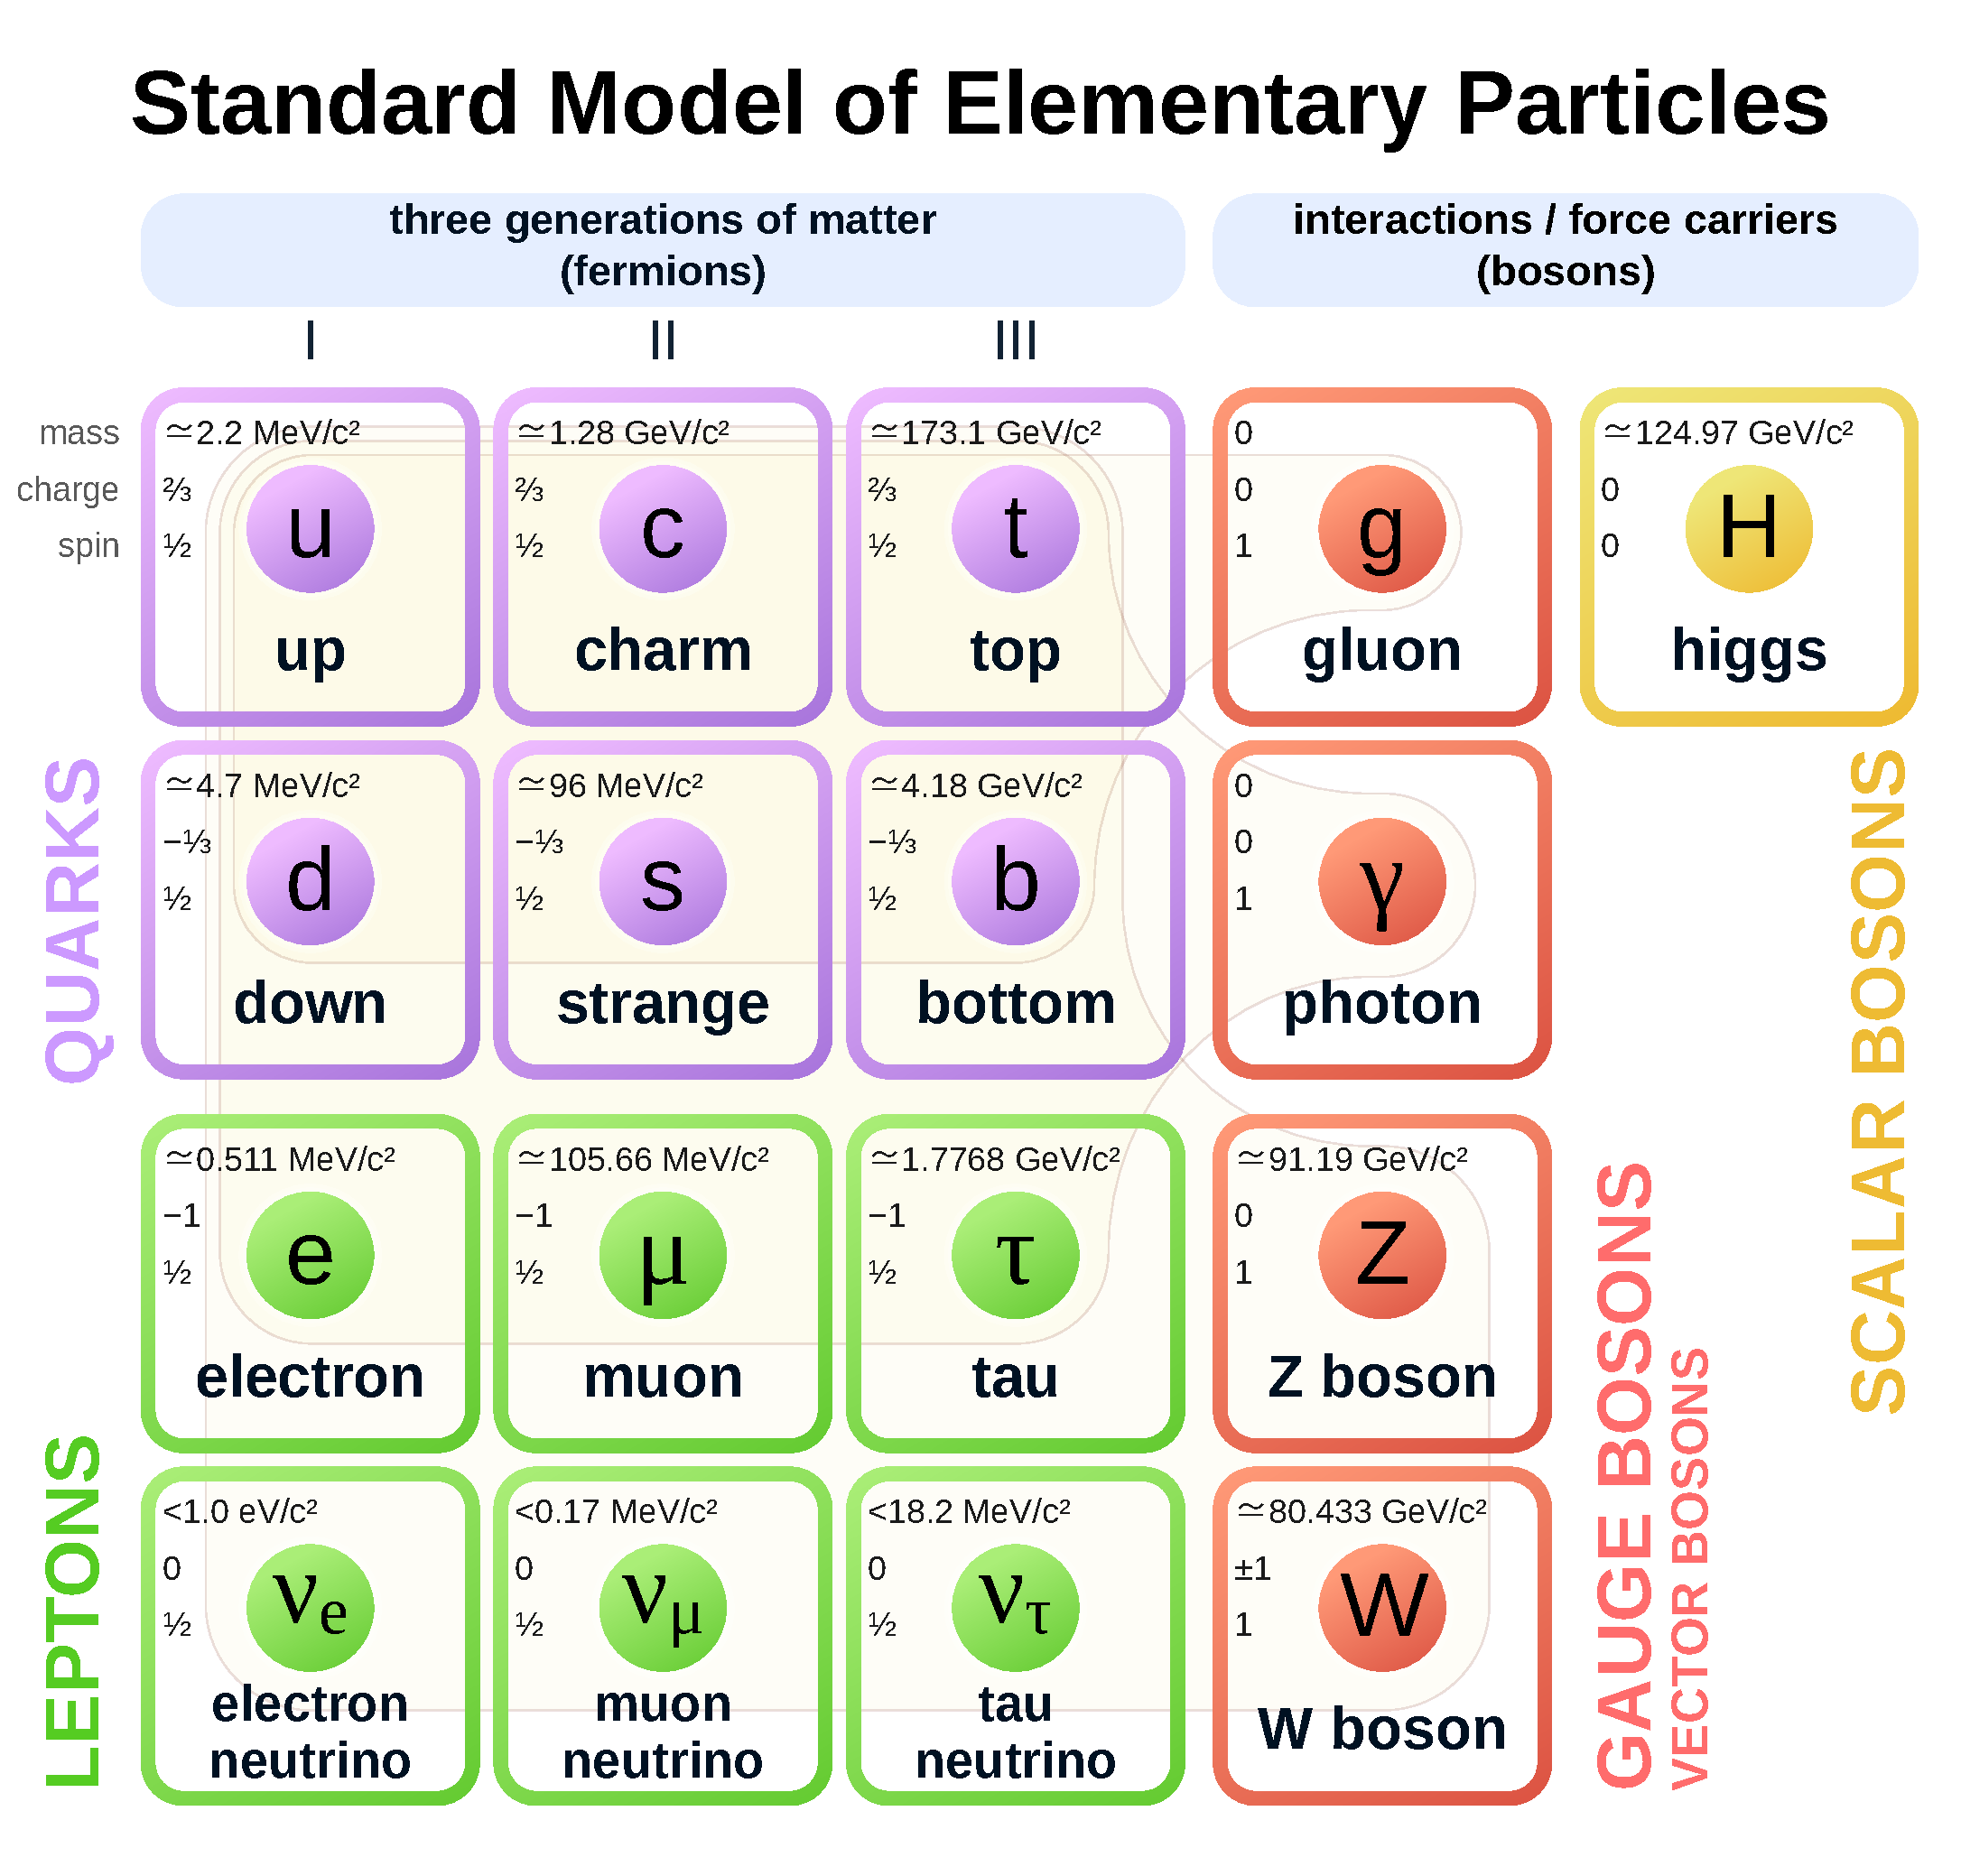
\includegraphics[width=\textwidth]{02standard_model.pdf}}
    \caption[The standard model.]{Fundamental particles in the Standard Model.
    Source: \hyperlink{commons.wikimedia.org/wiki/Main_Page}{Wikimedia Commons}.}
    \label{fig::10.02::standard_model}
\end{figure}

    % --+ How to study particle physics and DIS +-----------------------------------
Deep Inelastic Scattering (DIS) is the process used to investigate the interior of hadrons using leptons.
The process is similar to Rutherford scattering and provided the first experimental evidence of quarks.
DIS can be employed to delve even deeper into the structure of matter by utilising increasingly higher energies, thanks to Werner Heisenberg's uncertainty principle.

High-energy probes lead to asymptotic freedom, which is the property where the interactions between particles, such as quarks, become increasingly weak at shorter distances.
This implies that inside hadrons, quarks mostly move as free, non-interacting particles.
This allows for reliable calculation of event cross-sections in particle physics.

    % !TEX root = ../main.tex
% --+ Quantum Chromodynamics +--------------------------------------------------
Another important feature is colour confinement, which is the property of colour-charged particles that prevents their isolation.
Colour charge is the Quantum Chromodynamics (QCD) equivalent of electric charge.
There are three colour charges and their corresponding anticharges.
Quarks possess a single colour charge, while gluons, the force-mediators of the strong force, have a bi-colour charge.
In a state of equilibrium, the strong force confines quarks to be in close proximity, forming quark-antiquark pairs or 3-quark triplets in such a way that the net colour charge is neutral.

QCD describes these properties and models the quark strong interaction.
Similar to the electromagnetic force, the strength of the interaction is determined by the strong coupling constant \textalpha.
However, unlike the electromagnetic force, this constant weakens as distances decrease.

    % --+ What is this experiment +-------------------------------------------------
At a larger distance scale, or smaller resolution, confinement is expected to become visible.
The \textalpha value increases to values close to 1, and the perturbative treatment of QCD is not viable.
There is limited knowledge about the non-perturbative behaviour of QCD, and therefore, it mostly relies on phenomenological models at present.
The aim of the Run Group E (RG-E) experiment is to gather new data on the hadronic structure in Semi-Inclusive Deep Inelastic Scattering (SIDIS).
Through this experiment, we hope to gain further insight into quark propagation and hadron formation.


    % --+ Contents +------------------------------------------------------------
    % !TEX root = ../main.tex
\subsection{Deep Inelastic Scattering}
\label{10.10::deep_inelastic_scattering}
    In its simplest description, DIS refers to the scattering of an electron off a quark inside a nucleon.
    Figure \ref{fig::dis_diagram} displays the Feynman diagram illustrating DIS.
    The four-momentum of the nucleon is denoted by $P$, while that of the quark is represented by $p$.
    The initial and final four-momenta of the electron are given by $k$ and $k'$, respectively.
    When $k'$ is measured, the momentum transferred to the hadron system by the virtual photon is defined as $q = k - k'$.
    $q$ is a spacelike vector conventionally denoted as $q^2 = -Q^2$.

    \begin{figure}[h!]
        \centering\frame{
        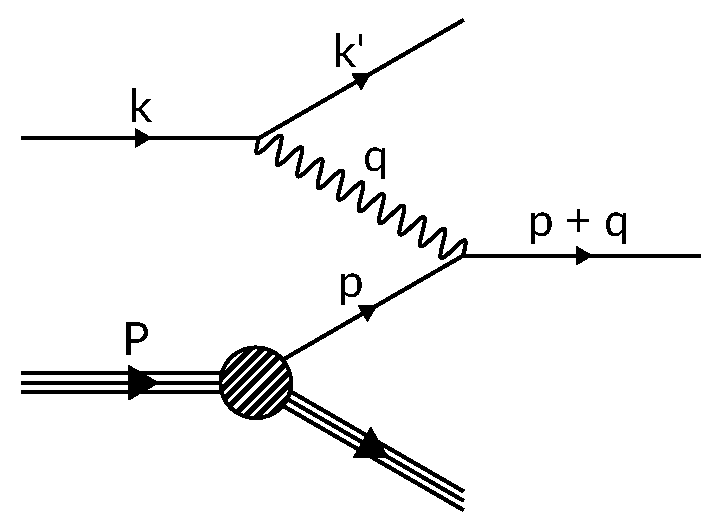
\includegraphics[width=0.6\textwidth]{10dis_diagram.pdf}}
        \caption[DIS in QCD.]{DIS in QCD. The diagram describes the stream of momentum in the scattering of a high energy electron off a quark. The quark's wave function is incorporated in the nucleon's wave function. Source: Own elaboration using \hyperlink{inkscape.org/}{Inkscape}.}
        \label{fig::dis_diagram}
    \end{figure}

    If $Q^2$ is sufficiently high, the quark is ejected from the nucleon.
    Soft processes, such as gluon emission and quark-antiquark pair production, then take place to neutralise the colour charge.
    This results in the transformation of the ejected quark into a jet of hadrons.
    The jet propagates in the direction of the transferred momentum from the electron.

    % !TEX root = ../main.tex
% --+ Approximating the cross section +-----------------------------------------
To approximate the cross section of electron-nucleon scattering, we will work in the center of mass reference frame.
In this frame, the electron and nucleon are moving towards each other with sufficient energy, allowing us to neglect the nucleon's mass.
As a result, the nucleon possesses nearly lightlike momentum along the collision axis.
Consequently, the constituent quarks of the nucleon also have nearly lightlike momenta that are nearly collinear to the nucleon's momentum.
Hence, as a first-order approximation, we can express the quark's momentum as
\begin{equation*}
    p = \xi P,
\end{equation*}
where $\xi$ represents the longitudinal fraction of the quark's momentum, and thus $0 < \xi < 1$.

In the leading-order approximation, we can also disregard gluon emission and exchange during the collision.
Therefore, the cross section of electron-nucleon scattering is equal to that of electron-quark scattering for a given $\xi$, multiplied by the probability that the nucleon contains a quark with a longitudinal momentum fraction of $\xi$, integrated over $\xi$.

This calculation encounters the issue that the probability of a nucleon containing a quark with a specific momentum cannot be computed within perturbative QCD.
It relies on the soft processes that determine the nucleon's structure as a composite system of quarks and gluons.
Consequently, we must consider this probability as an unknown function that needs to be measured in experiments.

Such probability functions are known as Parton Distribution Functions (PDFs).
A PDF can be assigned to various types of quarks, antiquarks, and gluons, and is incorporated into the nucleon's wave function.
For each parton $f$, its PDF is defined as
\begin{equation*}
    P_f = f_f(\xi)d\xi.
\end{equation*}
Therefore, the cross section for the inelastic scattering of an electron off a nucleon, within the leading-order approximation, can be expressed as
\begin{equation*}
    \sigma\left( e^-(k) p(P) \rightarrow e^-(k') X \right) =
            \int_0^1d\xi \sum_f f_f(\xi) \cdot
            \sigma\left( e^-(k) q_f(\xi P) \rightarrow e^-(k') + q_f(p') \right),
\end{equation*}
where $X$ denotes the final hadronic state.
It is important to remember that this equation does not provide an exact QCD prediction but represents the first-term expansion of $\alpha_s$.
This approximation is known as the parton model \cite{halzen1991}.

    % !TEX root = ../main.tex
\subsubsection{The Parton Model}
\label{sssec::parton_model}
    \begin{figure}[b!]
        \centering
        \frame{
        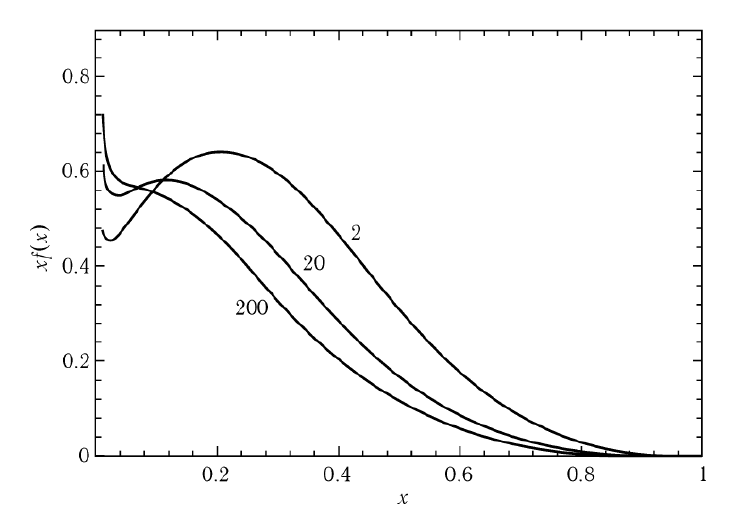
\includegraphics[width=0.8\textwidth]{12q2_dependence_u.png}}
        \caption[$Q^2$ dependence of $x$ PDF for the $u$ quark.]{Parton distribution functions $xf_f(x)$ for the $u$ quark at $Q = 2$, $Q = 20$, and $Q = 200$ GeV, showing the parton evolution effect according to the Altarelli-Parisi equations.} % NOTE. Can't find a source :(.
        \label{fig::q2dependenceu}
    \end{figure}

    In the parton model, the cross section is given by
    \begin{equation}
        \label{eq::parton_model_cross_section}
        \frac{d^2\sigma}{dxdy} \left( e^-p \rightarrow e^-X \right) =
                \left( \sum_f xf_f \left( x, Q^2 \right) Q_f^2 \right)
                \frac{2\pi\alpha s}{Q^4} \left( 1 + \left( 1 - y \right)^2 \right),
    \end{equation}
    where $s \equiv 2P\cdot k$, $Q_f$ represents the charge of parton $f$, and $x$ and $y$ are the Bjorken variables defined as
    \begin{equation*}
        x \equiv \frac{Q^2}{2P\cdot q}, \hspace{36pt} y \equiv \frac{2 P\cdot q}{s}.
    \end{equation*}
    In the nucleon's rest frame, $y = q^0/k^0$, and it represents the energy transferred to the hadron by the incoming electron.

    The PDFs in equation \eqref{eq::parton_model_cross_section} have a weak dependence on $Q^2$ due to gluon radiation.
    This leads to Bjorken scaling violation \cite{halzen1991}.
    When the structure functions are known for certain values of $Q^2$, they can be evolved to other values using the Dokshitzer-Gribov-Lipatov-Altarelli-Parisi (DGLAP) equations \cite{dokshitzer1991}.

    Figure \ref{fig::q2dependenceu} shows the predictions of the Altarelli-Parisi equations for the evolution of the PDFs with respect to $Q^2$.
    Partons with large $x$ tend to radiate and move towards states with lower $x$ values.
    Simultaneously, radiation generates new partons with low $x$ values.
    As $Q^2$ increases, the parton distributions decrease for large $x$ values while rapidly increasing for low $x$.
    At low $Q^2$, the wavelength of the virtual photon is too large to probe the partons directly, resulting in probing the proton as a whole.
    The precise range of validity for the QCD-extended parton model is not known, but it is assumed to be applicable for $Q^2 > 1 \text{ GeV}^2$, corresponding to a spatial resolution of approximately $0.2$ fm.

    % !TEX root = ../main.tex
\subsubsection{Strong Coupling Constant $\alpha_s$}
\label{10.13::strong_coupling_constant}
    Measuring the experimental value of $\alpha_s$ is crucial for perturbative QCD calculations.
    To achieve this, the overall scale of renormalisation needs to be determined.
    Typically, the mass of the neutral Bose particle $Z^0$, which is $91.19$ GeV, is chosen as the scale.
    Furthermore, the renormalisation scheme should be fixed, which defines the coupling constant at a specific scale.
    The experimental results for $\alpha_s$ can be seen in Figure \ref{fig::10.13::alpha_q_dependence}.

    \begin{figure}[t!]
        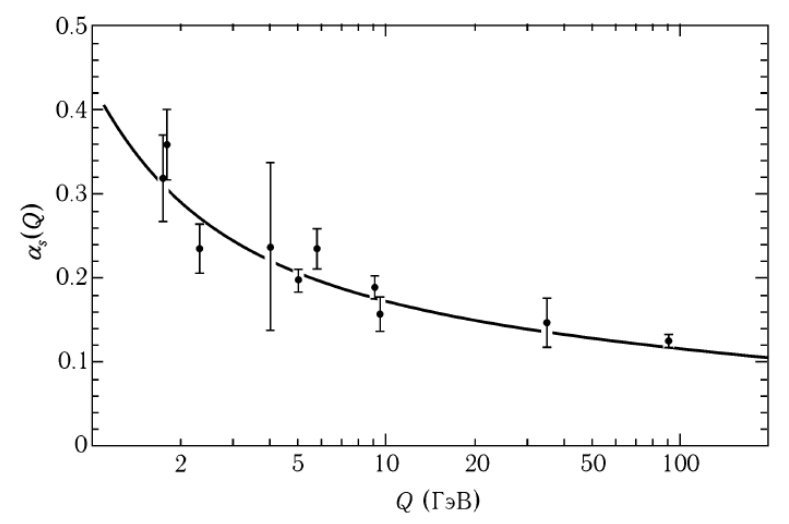
\includegraphics[width=0.8\textwidth]{13strong_coupling_constant_q.png}
        \caption[$\alpha_s$ dependence on $Q^2$]
        {Experimentally measured dependence of $\alpha_s$ on $Q$.
        The measured values are compared with the theoretical predictions of renormalised evolution with an initial value of $\alpha_s(m_z) = 0.117$ GeV.}
        % NOTE. Can't find a source :(.
        \label{fig::10.13::alpha_q_dependence}
    \end{figure}


    % % !TEX root = ../main.tex
\subsection{Semi-Inclusive Deep Inelastic Scattering}
\label{10.20::semi_inclusive_deep_inelastic_scattering}
    The previous section focused solely on the detection of the scattered electron in the inclusive reaction.
    However, in the case where one of the produced hadrons is identified, the event is referred to as semi-inclusive.
    The identification of this hadron provides information about the flavor of the quark that was struck.
    In SIDIS, it is possible to measure this flavor dependence.
    The identified hadrons in SIDIS are known as current fragments, and it is important to separate them in the analysis from the fragments originating from the target.

    % !TEX root = ../main.tex
\subsubsection{SIDIS Cross Section}
\label{10.21::sidis_cross_section}
    In SIDIS, the fragmentation process corresponds to very low $Q^2$ and is not calculable in perturbative QCD (pQCD).
    It is parameterised by fragmentation functions $D_f^h(Q^2, z)$, which measure the probability that an $f$-flavoured quark fragments into an $h$-type hadron with a fraction $z$ of the virtual photon energy ($E_h = z\nu$).

    In the quark-parton model, the cross section for $eN \rightarrow ehX$ is assumed to be the differential cross section from Equation \eqref{eq::10.12::parton_model_cross_section} multiplied by the fragmentation probability
    \begin{equation}
        \label{eq::10.21::fragmentation_probability}
        \frac{d^3\sigma(eN \rightarrow ehX)}{dxdQ^2dz} =
            \frac{d^2\sigma(eN \rightarrow eX)}{dxdQ^2} \cdot
            \frac{\sum_f e^2_f q_f(x,Q^2) D^h_f(Q^2,z)}{\sum_f e^2_f q_f(x,Q^2)}.
    \end{equation}

    It is assumed that the quasi-free scattering process and the fragmentary process are independent in the cross section.

    The hadron multiplicity per DIS event, denoted as $M_h(Q^2, z)$, is given by:
    \begin{equation*}
        M_h(Q^2,z) \equiv \frac{1}{\sigma} \frac{d^3\sigma(eN \rightarrow ehX)}{dQ^2dz} = \frac{\int dx \sum_f e^2_f q_f(x,Q^2) D^h_f(Q^2,z)}{\int dx \sum_f e^2_f q_f(x,Q^2)},
    \end{equation*}
    where $\sigma$ is the differential inclusive DIS cross section $\frac{d^2\sigma(eN \rightarrow eX)}{dxdQ^2}$.


    % % !TEX root = ../main.tex
\subsection{Hadronisation in the Nuclear Medium}
% --+ Introduction +------------------------------------------------------------
    Hadronisation is the process in which quarks and gluons form hadrons.
    When in the nuclear medium, this process is influenced by quark energy loss through two mediums: Gluon radiation and multiple quark-nucleon scattering.
    Moreover, hadron-nucleon interactions also affect the process if the hadronisation happens inside the nucleus.

    In the process, the primary experimental observable is the multiplicity of hadrons produced on a dense nucleus as compared to a light one -- such as deuterium.
    In the absence of attenuation from interactions with the medium, these two quantities should be identical, such that the ratio between multiplicities would be unity.
    The ratio of hadron multiplicities -- known as attenuation ratio -- is defined as
    \begin{equation*}
        R^h_{\text{att}}(z,\nu) = \frac
                {\left( \frac{1}{\sigma} \frac{d^2\sigma(eN \rightarrow ehX)}{dzd\nu} \right)_A}
                {\left( \frac{1}{\sigma} \frac{d^2\sigma(eN \rightarrow ehX)}{dzd\nu} \right)_{\prescript{2}{}{H}}},
    \end{equation*}
    where the derivative with respect to $Q^2$ is substituted with one with respect to $\nu$.
    The $\nu$ and $z$ dependence of this ratio can be used to study the nature of the hadron formation mechanism.

    One type of observable that can be isolated is the characteristic times for the distinct stages of the hadronisation process.
    The existence of these stages is dictated by two of the most fundamental properties in QCD.
    First, confinement: a coloured quark can only propagate for a limited distance.
    Second, causality: the equilibrium colour field of a hadron cannot be formed instantaneously.

    \input{10physics_motivation/virtual_photon_absorption}
    \input{10physics_motivation/production_time}
    \input{10physics_motivation/formation_time}


    \pagebreak

    % --+ Experiment +----------------------------------------------------------
    \graphicspath{{11experiment/img}}
    % !TEX root = ../main.tex
\section{Experiment}
\label{11::experiment}
    The Thomas Jefferson National Accelerator Facility (TJNAF) is a High Energy Physics (HEP) laboratory located in Newport News, Virginia, USA.
    For simplicity and to follow convention, the laboratory will be called Jefferson Lab (JLab) hereafter.
    At the site, there is a recirculating linear electron accelerator named the Continuous Electron Beam Accelerator Facility (CEBAF).
    This accelerator is capable of delivering a 12 GeV electron beam to four experimental Halls simultaneously: Halls A, B, C, and D.

    Different physics topics are studied in each of these halls.
    This thesis aims to provide a preparatory study for the Run Group E (RG-E) experiment, which will take place in Hall B, where the CEBAF Large Acceptance Spectrometer for operation at 12 GeV (CLAS12) is located.

    The first section provides a brief description of CEBAF at JLab.
    The second section then provides detailed information about CLAS12, including its central detector, forward detector, and offline event reconstruction.
    The third and final section discusses the RG-E experiment to be performed.

    % !TEX root = ../main.tex
\subsection{CEBAF}
\label{11.100::cebaf}
    \begin{figure}[b!]
        \centering\frame{
        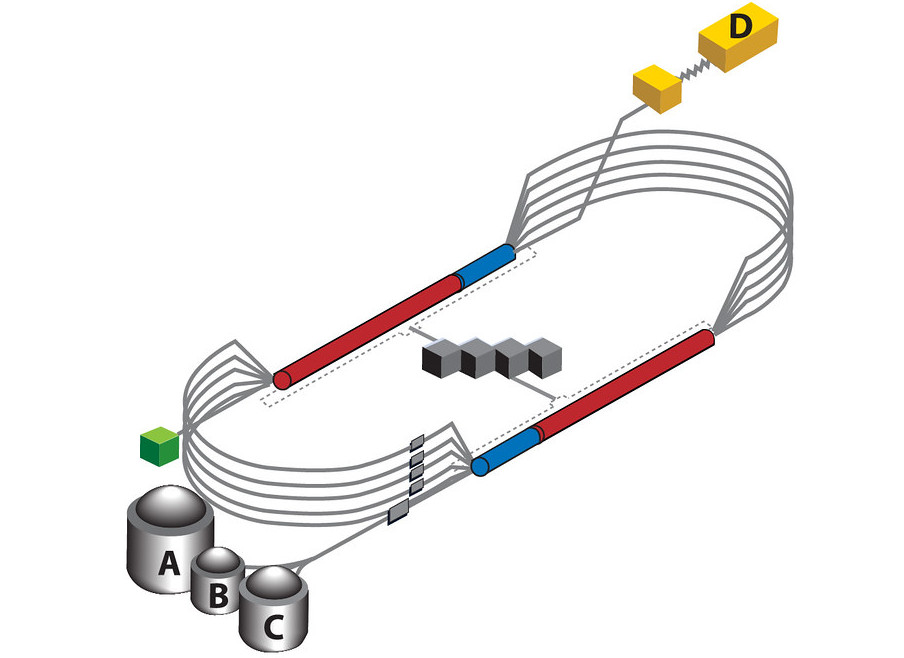
\includegraphics[width=\textwidth]{100cebaf_diagram.jpg}}
        \caption[CEBAF.]{Simplified representation of CEBAF.
        Source: \hyperlink{jlab.org/}{jlab.org}.}
        \label{fig::11.100::cebaf}
    \end{figure}

    CEBAF consists of a pair of 1.4-km-long antiparallel superconducting radio-frequency (RF) linear accelerators (linacs) constructed 8 meters below the surface.
    The two accelerators are connected by two 180-degree arcs, each with a radius of 80 meters \cite{leemann2001}.
    A schematic diagram illustrating the design of CEBAF is provided in Figure \ref{fig::11.100::cebaf}.

    The recirculating arcs are composed of five separate beamline sections, allowing the beam to traverse each linac up to five times.
    Within each linac, the energy gain of the beam ranges from 0.8 GeV to 1.2 GeV, resulting in a final beam energy of approximately 12 GeV.
    CEBAF is specifically designed for high-energy electron beam experiments aimed at studying the structure of mesons, nucleons, and nuclei \cite{rode2010}.

    % !TEX root = ../main.tex
\subsection{CLAS12}
\label{ssec::clas12}
    \begin{figure}[b!]
        \centering\frame{
        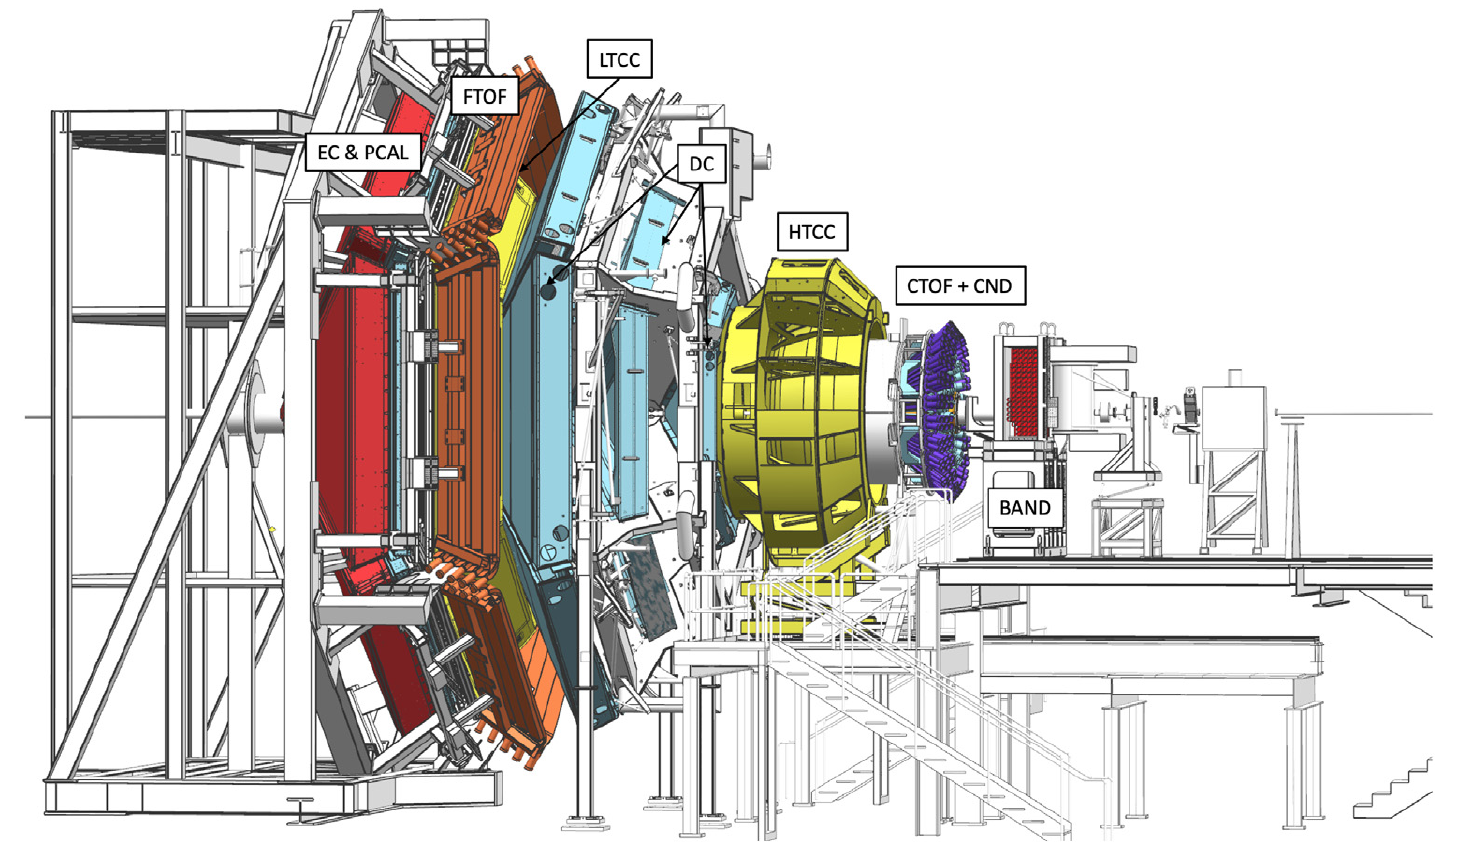
\includegraphics[width=\textwidth]{200clas12_diagram.png}}
        \caption[CLAS12.]{The CLAS12 detector in the Hall B beamline.
        The electron beam enters from the right and impinges on the target located in the center of the solenoid magnet shown at the right (upstream) end of CLAS12.
        The FD consists of the High Threshold Cherenkov Counter (HTCC) (yellow), the torus magnet (grey), the DC tracking system (light blue), and another set of Cherenkov counters (hidden), time-of-flight scintillation counters (brown), and Electromagnetic Calorimeters (ECs) (red).
        Between the HTCC and the torus, the Forward Tagger (FT) is installed.
        The CD consists of the Silicon Vertex Tracker (SVT) (hidden), which is surrounded by a Barrel Micromesh Tracker (BMT) (hidden), the Central Time-of-Flight (FTOF) system, and the Central Neutron Detector (CND) (blue).
        At the upstream end, a Back Angle Neutron Detector (BAND) (red) is installed.
        Source: \hyperlink{https://www.jlab.org/physics/hall-b/clas12}{CLAS12 wiki}.}
        \label{fig::clas12_diagram}
    \end{figure}

    The main detector in Hall B is CLAS12, used to study electro-induced nuclear and hadronic reactions \cite{burkert2020}.
    The spectrometer provides efficient detection of charged and neutral particles over a large fraction of the full solid angle.

    CLAS12 is based on two superconducting magnets: a solenoid magnet and a 5 T torus magnet.
    The detector is divided into two parts: the Forward Detector (FD) and the Central Detector (CD).
    The FD, aided by the torus magnet, covers the forward polar range from $5\degree$ up to $35\degree$, while the CD, aided by the solenoid magnet, covers the polar angles from $35\degree$ to $125\degree$.
    Both detectors have full azimuthal coverage.

    Trajectory reconstruction is performed using Drift Chambers (DC) in the forward direction, achieving a momentum resolution of less than $1\%$.
    In the central detector, trajectory reconstruction is done using a vertex tracker, resulting in a momentum resolution of less than $3\%$.
    Particle identification relies on Cherenkov counters, time-of-flight scintillators, and electromagnetic calorimeters \cite{burkert2020}.
    Fast triggering and high data-acquisition rates enable operation at a luminosity of $10^{35} \text{ cm}^{-2}\text{ s}^{-1}$ \cite{burkert2020}.

    A diagram of CLAS12 showing the position of each detector component is provided in Figure \ref{fig::clas12_diagram}.

    % !TEX root = ../main.tex
\subsubsection{Forward Detector}
\label{sssec::forward_detector}
    % The Forward Detector (FD) is an essential component of the CLAS12 spectrometer designed to detect particles scattered at small polar angles in the forward direction.
    % It consists of several subdetectors that play crucial roles in particle identification, tracking, and timing measurements.
    %
    % Based on its polar coverage, the FD can be divided into two: the Forward Tagger (FT) and the FD proper.
    % The former detects particles with a polar angle between $2.5\degree$ and $4.5\degree$.
    % The latter detects those with a polar angle between $5\degree$ and $35\degree$.
    % A detailed description of each subdetector systems is provided in the following paragraphs.
    %
    % The Forwards Micromegas Tracker (FMT) is part of the FD, but is not included in this list.
    % The detectors is explored in detail in Section \ref{ssec::forwardsmicromegastracker}.

    \input{11experiment/211htcc}
    \input{11experiment/212dc}
    \input{11experiment/213ltcc}
    \input{11experiment/214ftof}
    \input{11experiment/215rich}
    \input{11experiment/216ecal}
    \input{11experiment/217ft}

    % !TEX root = ../main.tex
\subsubsection{Central Detector (CD)}
\label{11.220::central_detector}
    In the CD, particles scattered from the target within the polar angle range of $35\degree$ to $125\degree$ are detected.
    The CD consists of various detectors that provide particle identification and tracking capabilities.
    Charged particles are detected in the Central Vertex Tracker (CVT) and the Central Time-of-Flight (CTOF) detector.
    Neutron detection is provided by the Central Neutron Detector (CND), which is located radially outside of the CVT and the CTOF.
    All detectors have full coverage in the azimuthal angle.

    \input{11experiment/221cvt}
    \input{11experiment/222ctof}
    \input{11experiment/223cnd}
    \input{11experiment/224band}

    % % !TEX root = ../main.tex
\subsubsection{Offline Reconstruction}
\label{11.230::offline_reconstruction}
% --+ CLARA +-------------------------------------------------------------------
    The CLAS12 reconstruction and analysis process is facilitated by a data-stream processing framework called CLARA.
    CLARA adopts a service-oriented architecture, allowing the construction of software applications using micro-services that are connected via data-stream pipes \cite{gyurgyan2016}.

    In this framework, each service plays a specific role.
    It receives input data, processes it according to its functionality, and produces output data.
    The input and output data are organised in tabular structures known as ``banks'', which are configured by the service developer to match the specific requirements of the service.

    The services within CLARA form a data-flow path, where the output of one service becomes the input for the next service in the sequence.
    This design enables a flexible and versatile data processing application, as each service can be individually improved or replaced without necessitating structural changes to the framework.

    To ensure consistency and modularity, the CLAS12 services are extensions of an abstract reconstruction engine.
    This engine provides common components such as initialisation and event processing methods, reducing the development complexity of individual micro-services and enforcing a uniform structure throughout the framework.

    By leveraging the CLARA framework, the CLAS12 experiment benefits from a modular and adaptable data processing pipeline, allowing for efficient reconstruction and analysis of the collected data.
    The service-oriented architecture and data-stream processing approach contribute to the flexibility, scalability, and maintainability of the CLAS12 software framework.

    \begin{figure}[b!]
        \centering\frame{
        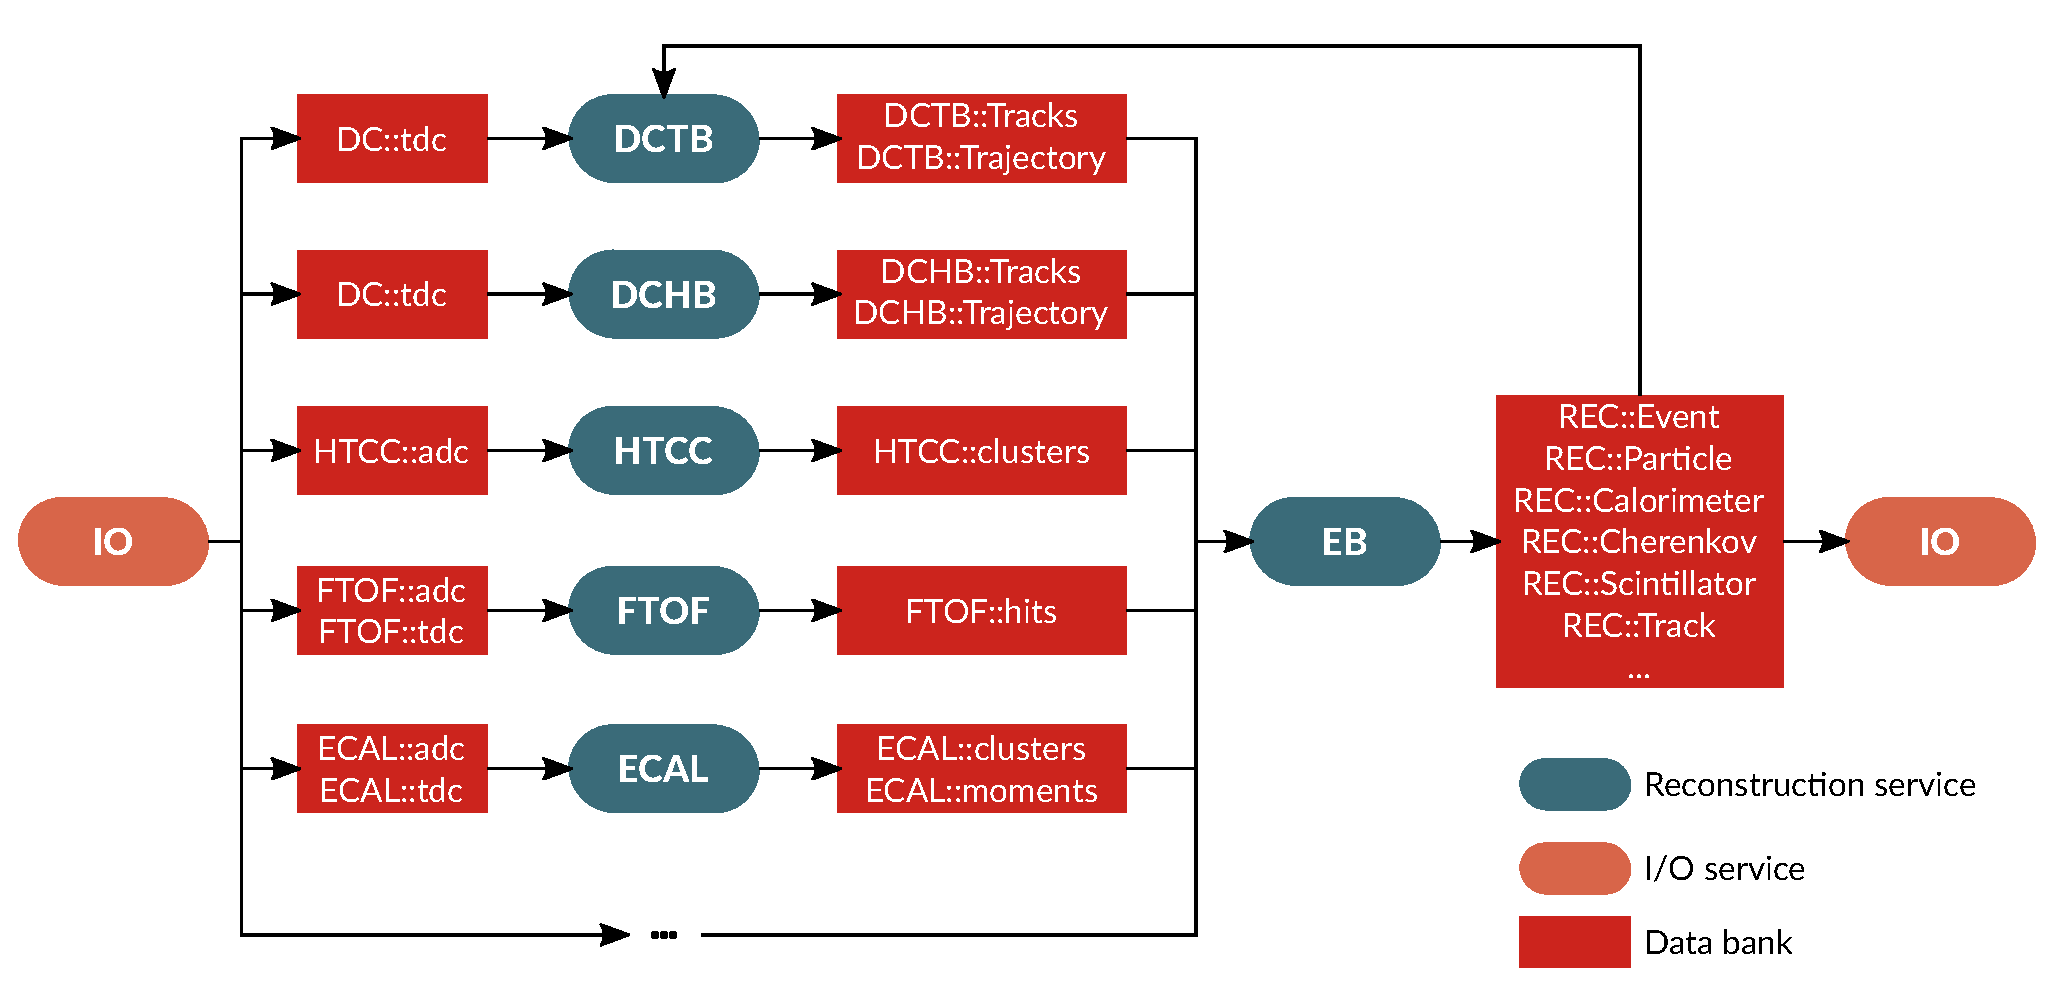
\includegraphics[width=\textwidth]{230recon_chain.pdf}}
        \caption[CLAS12 Reconstruction Chain.]{Graphical representation of the CLAS12 interdependencies between services and banks.
        The I/O service reads events from the input file and distributes them to the reconstruction services chain for processing.
        Each service reads the relevant banks, applies the reconstruction algorithm, and provides output banks that are passed to the next service in the chain.
        The Event Builder (EB) service is executed as last in the chain; it collects the relevant banks from all CLAS12 subsystems services and produces event, particle, and detector response banks that are written to the output file.
        Source: Own elaboration, using \href{https://inkscape.org/}{Inkscape}.}
        \label{fig::11.230::recon_chain}
    \end{figure}

% --+ CLAS12 reconstruction +---------------------------------------------------
    The CLAS12 data reconstruction process involves data reader services that access decoded detector data stored in banks.
    Each entry in the bank represents a decoded detector hit and contains information such as sector, layer, component, order, and digitised data like signal charge, amplitude, time, or pedestal.

    During the decoding stage, similar bank structures are created for various quantities required for event reconstruction, including hits, clusters, and tracks.
    Reconstruction algorithms specific to each CLAS12 subsystem fill these banks.
    The data persistence service appends and writes these banks to a file for later analysis.

    The reconstruction algorithms are implemented as services that operate on input banks and produce output banks, which are then passed to subsequent algorithms in the reconstruction chain.
    The order in which the services are chained reflects the overall sequence of CLAS12 event reconstruction and the dependencies between subsystems.

    The first step is the reconstruction of charged particle tracks in the Central and Forward Detector tracking systems, based on the recorded hit positions in the respective detectors.
    This process is known as ``hit-based'' tracking.

    Simultaneously, hits recorded in other detectors are processed to reconstruct the energy and time of the associated particle interactions.
    The Event Builder (EB) service matches these reconstructed quantities with the tracks based on position and time information.
    Hits that are not matched to any track are retained as neutral particle candidates.
    The EB also determines the event ``start time'' and identifies the reconstructed particles.

    Once the event start time is determined, a second iteration of forward tracking, known as ``time-based'' tracking, can be performed.
    This iteration incorporates the drift times in the Drift Chambers, providing improved tracking precision \cite{ziegler2020}.

    An overview of the composition of reconstruction application services, depicting the dependencies between the services, can be found in Figure \ref{fig::11.230::recon_chain}.

    \input{11experiment/231tracking}
    \input{11experiment/232particle_identification}


    % !TEX root = ../main.tex
\subsection{RG-E Experiment} \label{ssec::rgeexperiment}
    The Run Group E (RG-E) experiment aims to measure the hadronic multiplicity ratio between different nuclei and deuterium.
    To do this, a double-target system is being built to be used in Hall B.
    The system will allow a precise comparison of a deuterium target and heavy solid targets, like carbon, aluminium, copper, tin, lead, etc.
    The experiment aims to further the understanding of hadronisation in the nuclear medium, colour transparency, and nuclear short-range correlations.

    During data acquisition, the cryo-target (deuterium) and a solid target will be exposed to the electron beam simultaneously.
    To minimise acceptance correction difference between targets, we aim to keep the distance between them as low as possible -- as long as we can differentiate between the targets in reconstruction.
    Part of this thesis' work involves improving offline reconstruction before the experiment to reduce this distance, which can be read in chapter \ref{sec::fmtalignmentandreconstruction}.

    Positioning both targets in the beam simultaneously allows us to cancel time-dependent systematic effects o increase the precision of final results.
    These include effects such as drifting gains and inefficient detector channels in the measurement of ratio-like observables.
    Then, since the target system will be in a vacuum, the switching between solid targets will need to be performed remotely.
    Additionally, it needs to be done as quickly as possible, to maximise the beam time of the experiment.

    The double target system will be able to switch between up to five different solid targets.
    The previous EG2 experiment performed on the former CLAS showed that the design of the double target system has significant advantages to reduce the systematic uncertainties \cite{hakobyan2008}.
    The principle of the target system is to have the solid targets installed on a carbon fibre band which slides on torlon rails.
    The band is moved by a piezo-motor, which -- like all other chosen materials -- is insensitive to magnetic fields.
    The design proposed can be seen in figure \ref{fig::double_target}.

    \begin{figure}[b!]
        \centering\frame{
        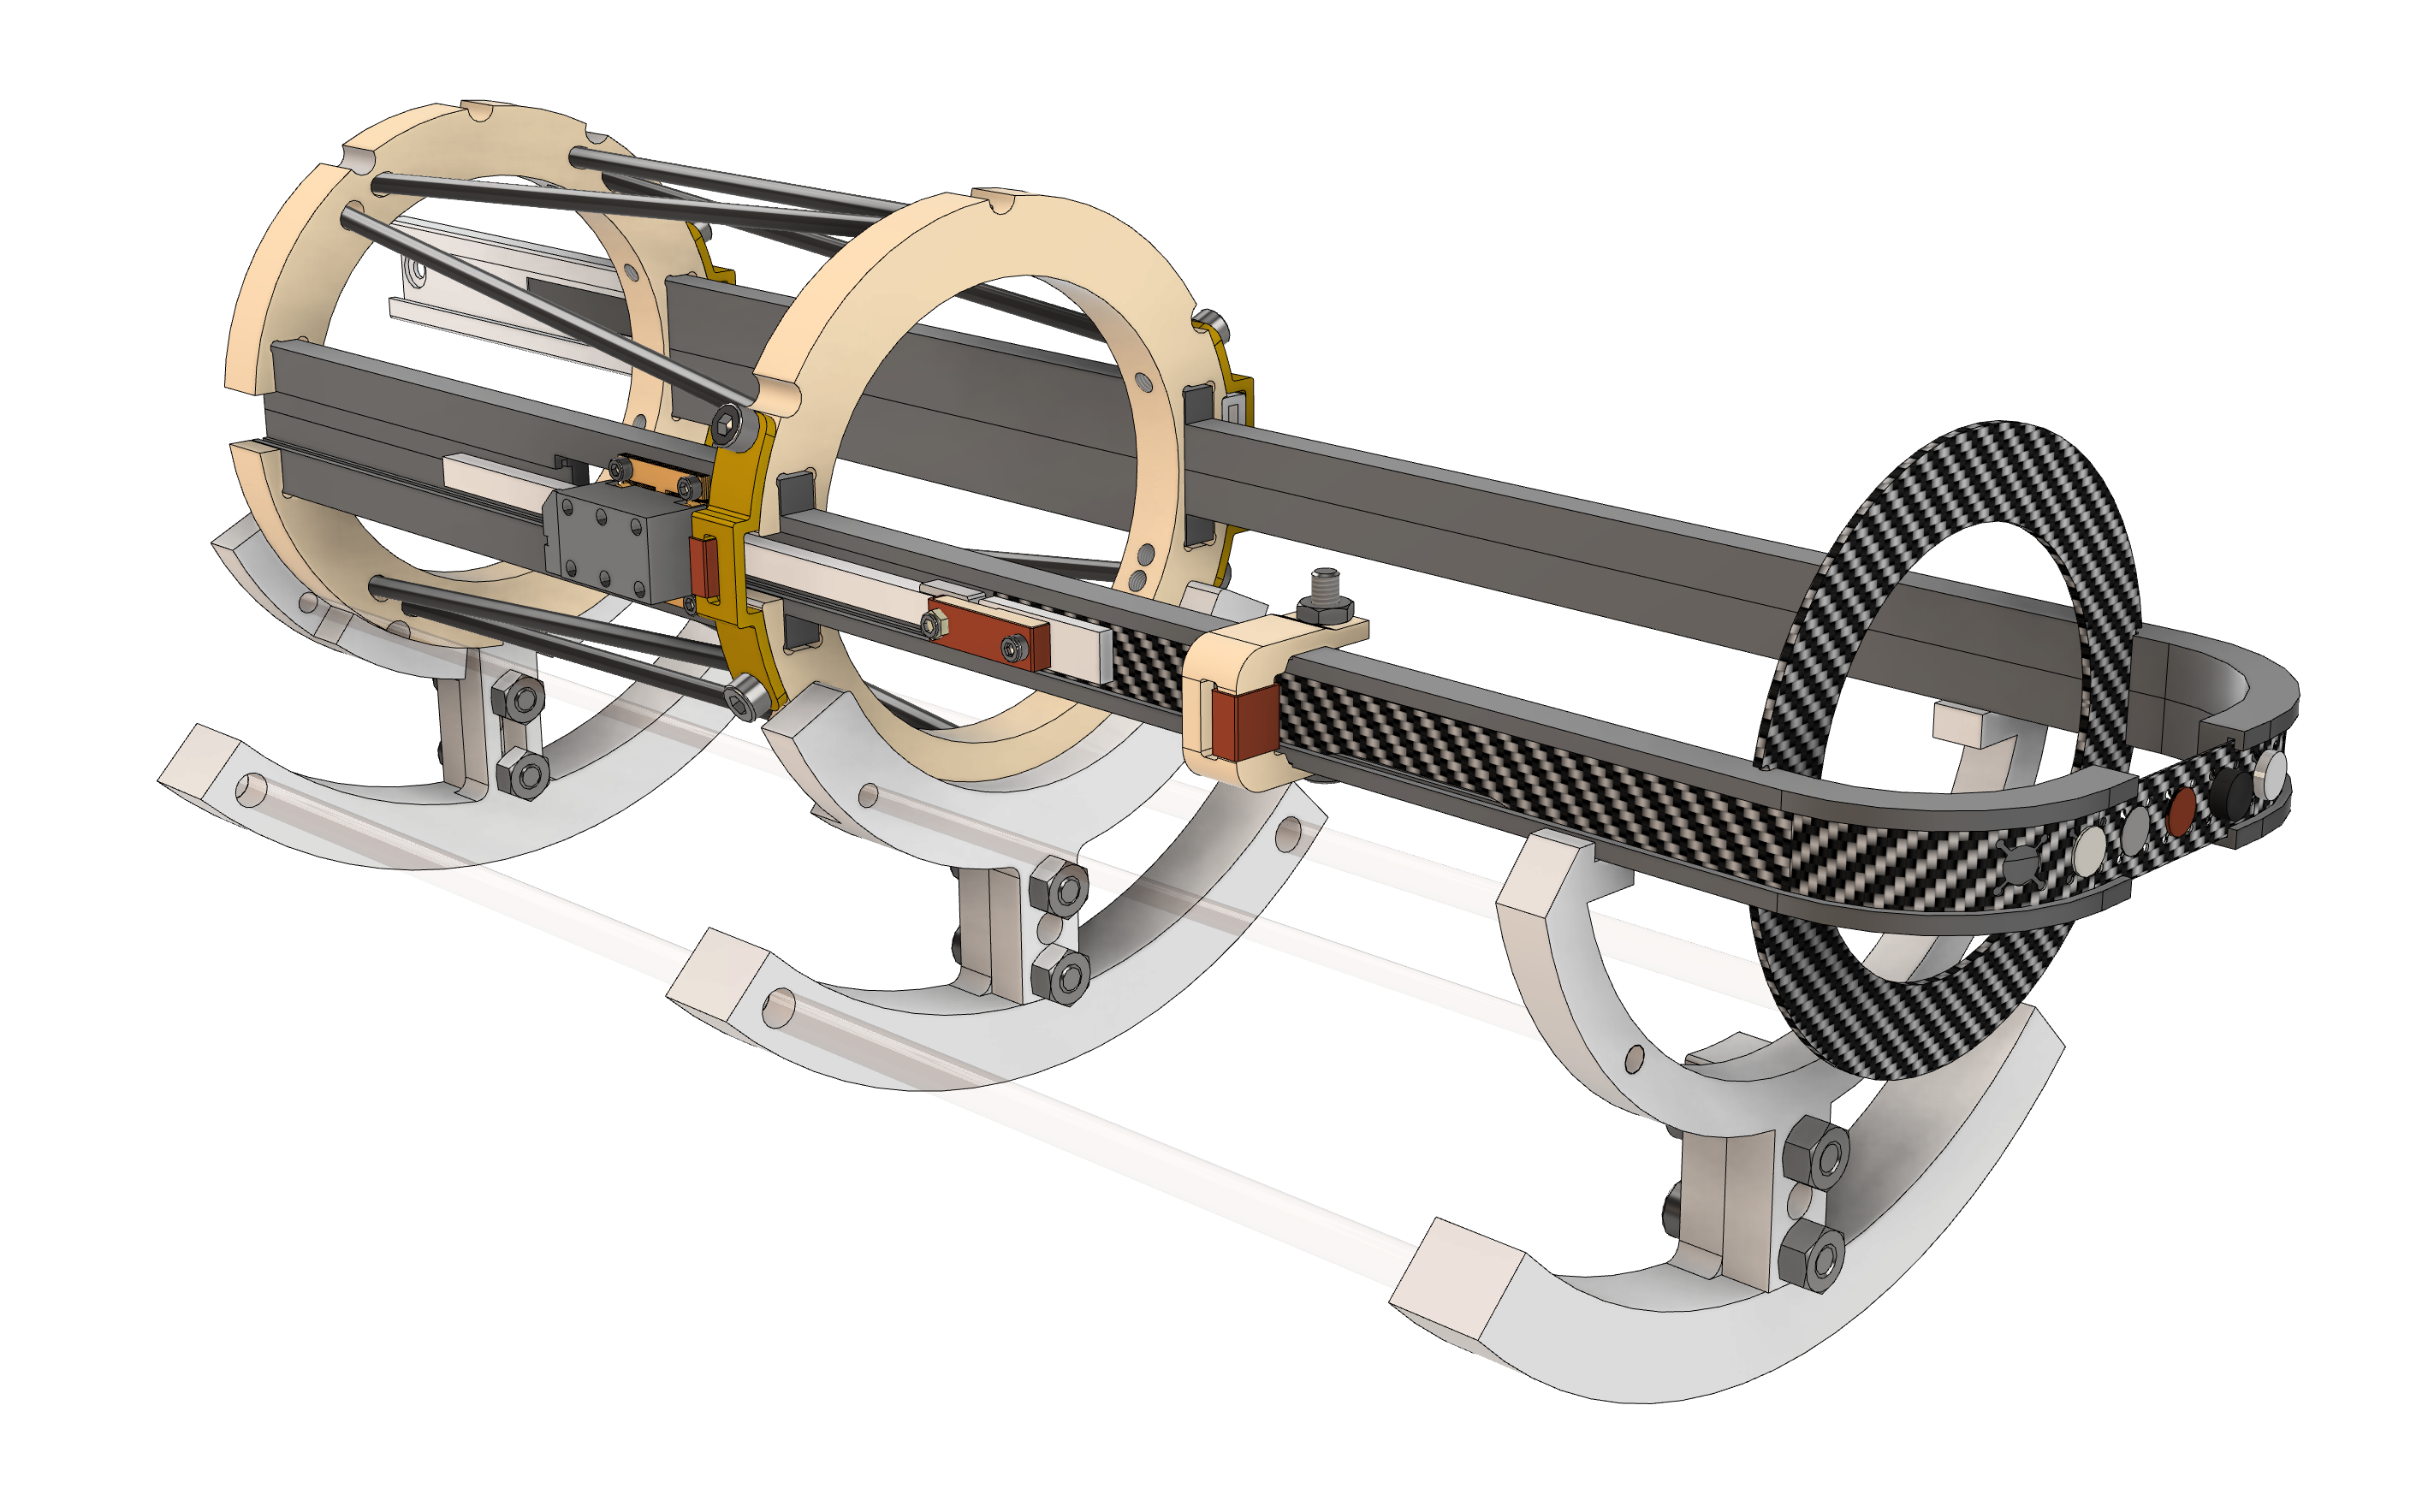
\includegraphics[width=\textwidth]{11experiment/img/30double_target.png}}
        \caption[Double-target system.]{Double-target system CAD render.}
        \label{fig::double_target}
    \end{figure}

    To ensure the adequate operation of the target, several tests were performed.
    These include movement under vacuum and high magnetic field, radiation hardness of the selected materials, and heat removal tests which secure that target remain far below melting point.

    % !TEX root = ../main.tex
\subsubsection{Slow Control System} \label{sssec::slowcontrolsystem}
% --+ What is slow control +----------------------------------------------------
    A modern experimental physics experiment usually involves many of moving parts and complex components that need constant monitoring and calibration.
    This is in addition to the constant data taking necessary.
    The process of automating this task is made via slow controls systems.
    These systems usually integrate a whole detector and experiment into one complex interface, allowing for easy access and maintenance.

% --+ What is EPICS +-----------------------------------------------------------
    The standard framework to do this in the context of HEP is the Experimental Physics and Industrial Control System (EPICS).
    EPICS was developed in the Los Alamos National laboratory (ANL) to provide data acquisition and control to this type of experiments.
    The framework provides a distributed process control that includes software communication, functional subsystems for data acquisition, supervisory control, closed loop control, channel archiving, and alarm management \cite{dalesio1991}.
    Like many HEP experiments, CLAS12's slow control system is based on EPICS \cite{boyarinov2020}.

% --+ EPICS installation on raspi +---------------------------------------------
    To allow the integration of the RG-E target on the CLAS12 slow controls system, an EPICS support module and Input / Output Controller (IOC) was developed by the author.
    This module wasn't made from scratch, as the motor developers made a generic support module for Galil motors \cite{farnswort2009}.
    This system proved to support all that was necessary for the movement of the RG-E target system, only requiring the removal of unnecessary features and the addition of database variables relevant to the experiment.
    % NOTE. This chapter doesn't involve the integration of thermocouples, as that is left as future work.

    The Process Variables (PVs) added to the EPICS module are listed, along with a short description of each.
    Each of these can be viewed and edited at the user-defined records database, which is at

    \begin{center}
        \texttt{\$EPICS\_BASE/support/galil/3-6/db/galil\_userdef\_records.template}.
    \end{center}

    \paragraph{Analog Input (\texttt{ai})}
        The normal use for this record type is to obtain an analog value from hardware and then convert it to engineering units \cite{stanley1998}.
        The record can also be used to write constants to be read from the database, such that they can be changed in runtime.

        \subparagraph{\texttt{DMC01:A\_curr\_pos}.}
            Current position of the band.
            Displayed at the GUI and used for internal calculations.

        \subparagraph{\texttt{DMC01:A\_home}.}
            Position of the home.
            Displayed at the GUI and used for calculations.

        \subparagraph{\texttt{DMC01:A\_pos\#}.}
            \# is a number from 1 to 7.
            Positions of each of the seven targets.
            Displayed at the GUI and used for calculations.

        \subparagraph{\texttt{DMC01:A\_lowlimit}.}
            Position of the low limit.
            If \texttt{DMC01:A\_curr\_pos} is lesser than this value, a major alarm is fired.

        \subparagraph{\texttt{DMC01:A\_highlimit}.}
            Position of the high limit.
            If \texttt{DMC01:A\_curr\_pos} is greater than this value, a major alarm is fired.

        \subparagraph{\texttt{DMC01:A\_tolerance}.}
            Equivalence tolerance for the position of each target and the position of the band.
            It defines a valid range around the target position.

        \subparagraph{\texttt{DMC01:COMMERR\_STATUS}.}
            Variable that is true when there's a communication error with the controller and false otherwise.
            Used for triggering a communication alarm.

        \subparagraph{\texttt{IOC01:SR\_i\_am\_alive}.}
            Variable that is true when the IOC is up and running, false otherwise.
            Used for triggering a communication alarm.

    \paragraph{Analog Output (\texttt{ao})}
        The normal use for this record type is to output values to digital-analog converters.
        The desired output can be controlled by either an operator or a state program, or it can be fetched from another record \cite{stanley1998}.

        \subparagraph{\texttt{DMC01:A\_go\_home}.}
            Command to move the band to the home position, as defined in \texttt{DMC01:A\_home}.

        \subparagraph{\texttt{DMC01:A\_go\_pos\#}.}
            Command to move the band to the position of target \#, as defined in \texttt{DMC01:A\_pos\#}.

    \paragraph{Calculation (\texttt{calc})}
        The calculation or ``Calc'' record is used to perform algebraic, relational, and logical operations on values retrieved from other records.
        The result of its operations can then be accessed by another record so that it can be used \cite{stanley1998}.
        In the context of the RG-E target, each calculation returns a number from 0 to 11.
        This number represent the state the target is in, and is later used by a Select PV.

        \subparagraph{\texttt{DMC01:A\_at\_pos\#}.}
            Calculation that checks if the band position is equal to that of target \# in \texttt{DMC01:A\_pos\#}, within the tolerance margin \texttt{DMC01:A\_tolerance}.
            If it is, it returns \#.
            Otherwise, it returns 0.

        \subparagraph{\texttt{DMC01:A\_at\_home}.}
            Calculation that checks if the band position is equal to the home position in \texttt{DMC01:A\_home}, within the tolerance margin defined by the tolerance.
            If it is, it returns 8.
            Otherwise, it returns 0.

        \subparagraph{\texttt{DMC01:A\_moving}.}
            Calculation that checks if the target is moving by checking the motor PV \texttt{DMC01:A.MOVN}.
            If it is, it returns 9.
            Otherwise, it returns 0.

        \subparagraph{\texttt{DMC01:A\_at\_lowlimit}.}
            Calculation that checks if the band position is lesser than the low limit \texttt{DMC01:A\_lowlimit}.
            If it is, it returns 10.
            Otherwise, it returns 0.

        \subparagraph{\texttt{DMC01:A\_at\_highlimit}.}
            Calculation that checks if the band position is greater than the high limit \texttt{DMC01:A\_highlimit}.
            If it is, it returns 11.
            Otherwise, it returns 0.

    \paragraph{Select (\texttt{sel})}
        The select record computes a value based on input obtained from up to 12 locations.
        By default, it is equal to the highest value among its input PVs \cite{stanley1998}.

        \subparagraph{\texttt{DMC01:A\_sel\_tgttype}.}
            This record returns the highest value between the previously defined calculations.
            Thus, it associates the values returned to a state of the target.
            By convention, this PV assumes that \emph{no more than one \texttt{calc} is greater than 0}.
            This assumptions holds as long as \texttt{DMC01:A\_tolerance} is not set higher than half the distance between targets and between the targets and the lower and higher limits.

    \paragraph{Multi-Bit Binary Input (\texttt{mbbi})}
        The normal use for the multi-bit binary input record is to read multiple bit inputs from hardware.
        The binary value represents a state from a range of up to 16 states.
        The multi-bit input record interfaces with devices that use more than one bit \cite{stanley1998}.

        \subparagraph{\texttt{DMC01:A\_tgttype}.}
            This \texttt{mbbi} encodes the output of \texttt{DMC01:A\_sel\_tgttype} to a string and alarm level.
            The encoding is specified in table \ref{tab::tgttypespv}.

    \begin{table}[b!]
        \caption{Names and alarm levels for the different values of the PV \texttt{DMC01:A\_tgttype}.}

        \begin{center}
            \begin{tabularx}{220pt}{lll}
                \hline
                \textbf{Value} & \textbf{Name} & \textbf{Alarm Severity} \\
                \hline
                 0             & Not Moving    & Major                   \\
                 1             & Target 1      & No alarm                \\
                 2             & Target 2      & No alarm                \\
                 3             & Target 3      & No alarm                \\
                 4             & Target 4      & No alarm                \\
                 5             & Target 5      & No alarm                \\
                 6             & Target 6      & No alarm                \\
                 7             & Target 7      & No alarm                \\
                 8             & Home          & No alarm                \\
                 9             & Moving        & Minor                   \\
                10             & Low Limit     & Major                   \\
                11             & High Limit    & Major                   \\
                \hline
            \end{tabularx}
        \end{center}
        \label{tab::tgttypespv}
    \end{table}

    The RG-E IOC, along with the complete set of EPICS support modules necessary to run it, can be found at

    \begin{center}
        \hyperlink{https://github.com/bleaktwig/rge-epics-support}{\texttt{https://github.com/bleaktwig/rge-epics-support}}.
    \end{center}

    \paragraph{CS-Studio}
        The Graphical User Interface (GUI) of CLAS12 EPICS is based on the Control System Studio (CS-Studio) toolkit.
        CS-Studio is used to monitor and operate large scale control systems, and is based on the eclipse Rich Client Platform (RCP) framework \cite{kasemir2007}.
        In order to integrate the RG-E target system into CLAS12 EPICS, a CS-Studio screen needed to be developed.

        The set of requirements the screen needed to fulfil are listed.
        These requirements are based both on the specifications of the physics experiments and the needs of the electronics team behind the target.
        \begin{itemize}
            \item
                Buttons to move the target band to the targets and a home location.
            \item
                A Button to stop the target band in case of emergency.
            \item
                A status check on the position of the target band.
            \item
                Alarm handling for the case when the band moves beyond low and high limits.
            \item
                Alarm handling for the IOC and communication problems.
        \end{itemize}
        These requirements were implemented in the screen, which can be seen in figure \ref{fig::rge_motorx}.
        In addition to the buttons, text displays show the position of each target in the band.
        LED displays to the right of these light up green when the band position matches the target position, within a tolerance defined in the database.
        Finally, four LED displays are laid in to the right of the two IOC statuses and the low and high limits.
        These show alarm conditions, acting in tandem with the CLAS12 Slow Control alarm system to alert the user of a problem.

        \begin{figure}[t!]
            \centering\frame{
            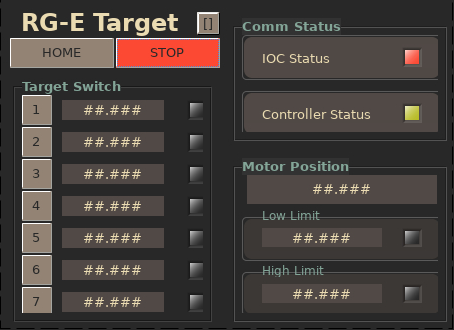
\includegraphics[]{11experiment/img/31motorx_rge.png}}
            \caption[RG-E CS-Studio main screen]{RG-E CS-Studio main screen. The HOME and A, B, C, etc buttons move the target strip to the corresponding location, the STOP button is an emergency, instant stop of the target system, and the Motor Screens button allows the user to open additional motor screens.}
            \label{fig::rge_motorx}
        \end{figure}

        In addition to this screen, other screens can be accessed through the Motor Screens menu button.
        These screens are part of the motor EPICS support module, and are left in case any debugging is necessary.
        These screens include a screen that allows for manual motor movement, a motor setup screen, a direct Command Line Interface (CLI) with the motor, and an amplifier configuration screen.
        All of these screens were developed by the Galil EPICS team \cite{farnswort2009}.

        For the user's comfort, the GUI was coloured using the Gruvbox colour palette.
        This palette is designed to keep colours easily distinguishable, contrast enough, while being pleasing for the eyes.
        Gruvbox can be found on GitHub at

        \begin{center}
            \hyperlink{https://github.com/morhetz/gruvbox}{\texttt{https://github.com/morhetz/gruvbox}}.
        \end{center}

    \paragraph{Alarm System}
        To secure the good functioning of the CLAS12 detector, all its subsystems controlled via EPICS contain PVs that specify alarm conditions.
        A centralised alarm system displays these alarms, together with their severity, associated subsystems, and pre-written guidance on how to react to them.
        For each experiment with a non-trivial target done in Hall B, the target system requires its own list of alarms.

        For the RG-E target, the set of alarms implemented and their related PVs are listed in table \ref{tab::alarmspv}.

        \begin{table}[b!]
            \caption{Alarm names, triggers, and severities for the RG-E target slow control system.}

            \begin{center}
                \begin{tabularx}{360pt}{llX}
                    \hline
                    \textbf{Name}          & \textbf{Trigger}                     & \textbf{Severity} \\
                    \hline
                    Band is not moving     & \texttt{DMC01:A\_tgttype}       =  0 & Major             \\
                    Band is moving         & \texttt{DMC01:A\_tgttype}       =  9 & Minor             \\
                    Band beyond low limit  & \texttt{DMC01:A\_tgttype}       = 10 & Major             \\
                    Band beyond high limit & \texttt{DMC01:A\_tgttype}       = 11 & Major             \\
                    Controller comm. error & \texttt{DMC01:COMMERR\_STATUS}  =  1 & Major             \\
                    IOC comm. error        & \texttt{IOC01:SR\_i\_am\_alive} =  0 & Major             \\
                    \hline
                \end{tabularx}
                \label{tab::alarmspv}
            \end{center}
        \end{table}



    \pagebreak

    % --+ FMT Alignment +-------------------------------------------------------
    \graphicspath{{12fmt_alignment/img}}
    % !TEX root = ../main.tex
\section{FMT Alignment and Reconstruction}
\label{sec::fmt_alignment_and_reconstruction}
    In paper, the Forwards Micromegas Tracker (FMT) offers a 3 to 10-fold increase in resolution when compared to DC \cite{aune2009}.
    Achieving this improvement requires work on the alignment and calibration of the detector, as well as the reconstruction from its data.
    This chapter focuses on the work carried out in this endeavor, specifically addressing alignment and reconstruction.

    The first section provides a detailed description of Micromegas detectors in general and the FMT in particular.
    Subsequently, the second and third sections discuss the efforts made in alignment and reconstruction, respectively.
    Finally, the fourth and final section of the chapter elaborates on the resolution improvement resulting from this work.

    % !TEX root = ../main.tex
\subsection{Forwards MicroMegas Tracker}
\label{12.10::forwards_micromegas_tracker}
% --+ Micromegas +--------------------------------------------------------------
    \begin{figure}[b!]
        \centering\frame{
        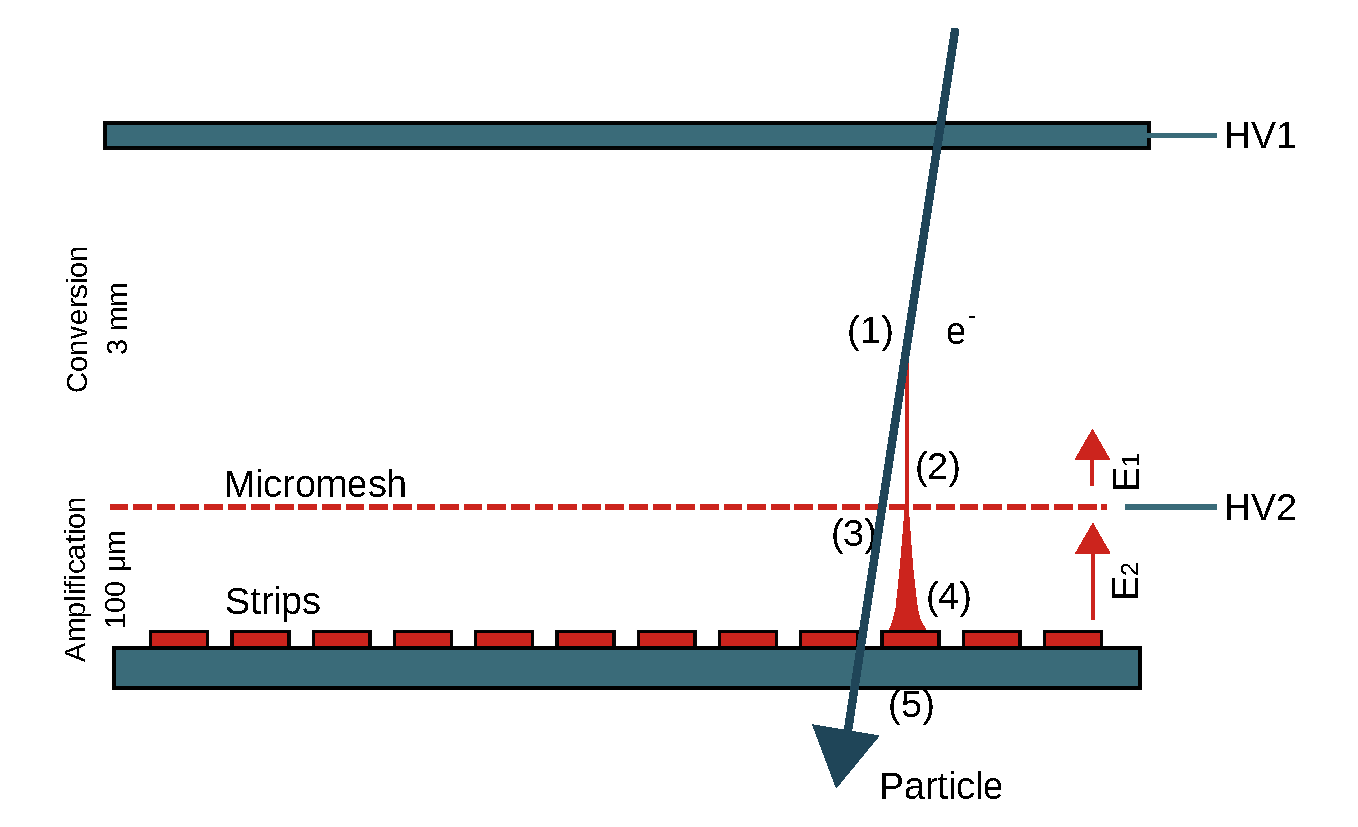
\includegraphics[width=\textwidth]{10mm_principle.pdf}}
        \caption[MM working principle.]{MicroMegas working principle.
        Source: Re-render of original illustration by \cite{giomataris1996}.}
        \label{fig::12.10::micromegas_principle}
    \end{figure}

    A Micro-Mesh Gaseous Detector or MicroMegas (MM) is a gaseous particle detector that is derived from wire chambers.
    These types of detectors are commonly used in experimental physics for detecting ionising particles.
    The MM detector offers very precise temporal and spatial resolution, on the order of 100 nanoseconds and below 100 micrometers \cite{giomataris1996}.

    The detector operates by amplifying the charges created by ionisation in the gas volume.
    Its volume is divided into two parts by a metallic micro-mesh placed less than 150 micrometers away from the readout electrode or strip.

    To illustrate this process, refer to Figure \ref{fig::12.10::micromegas_principle}.

    When a particle passes through the detector, it ionises the gas atoms by stripping an electron, resulting in an electron-ion pair (1).
    An electric field, denoted as $\text{E}_1$, is applied to the gas, causing the electron to drift towards the amplification electrode (2) while the ion moves towards the cathode.
    As the electron crosses the mesh (3), it enters a strong electric field, denoted as $\text{E}_2$, triggering an avalanche effect (4).
    This produces a significant signal at the readout strip (5), which can then be stored for reconstruction \cite{giomataris1996}.

% --+ Micromegas in CLAS12 +----------------------------------------------------
    Inside the CLAS12 detector, a diverse set of tracking detectors is utilised to determine the positions and momenta of particles at different points along their trajectories.
    The proximity of these detectors to the particle source directly correlates to the precision achieved in determining the position and momentum at the interaction vertex, which refers to the point where the particle was generated.
    To optimise this precision, the MicroMegas Vertex Tracker (MVT) in CLAS12 is positioned as close as feasible to the target, as depicted in Figure \ref{fig::12.10::micromegas_vertex_tracker}.

    \begin{figure}[b!]
        \centering\frame{
        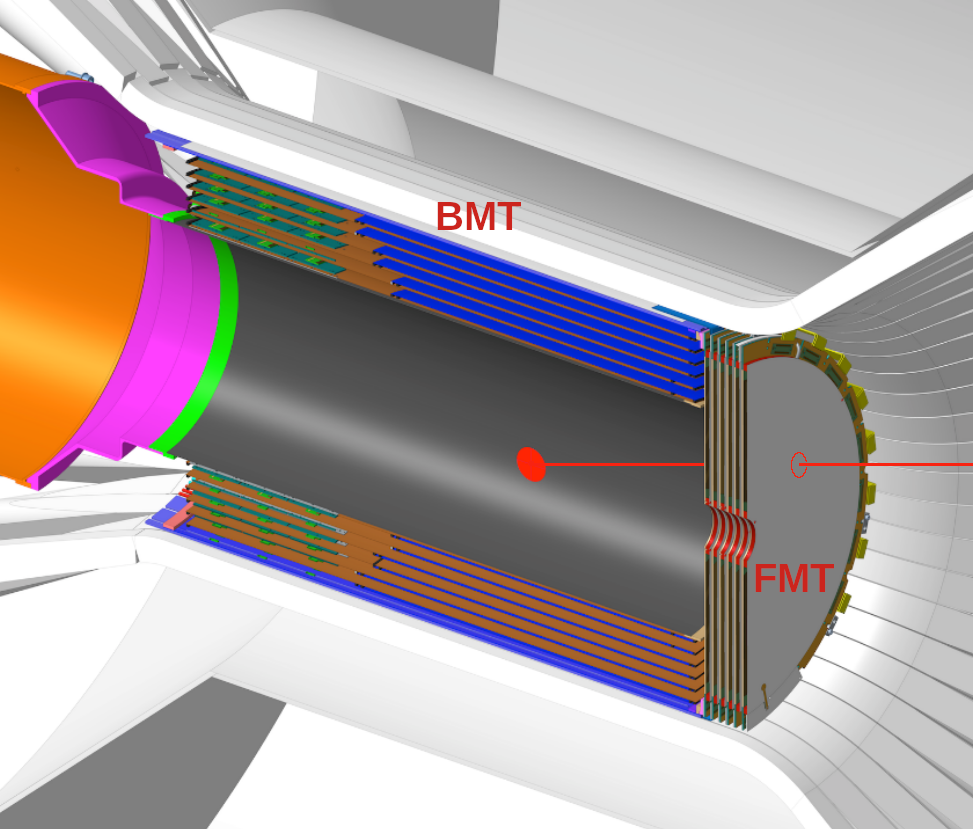
\includegraphics[scale=0.5]{10mvt.png}}
        \caption[MVT detector.]{MVT detector.
        The red dot denotes the $z=0$ point in the beamline, the red line denotes an arbitrary track coming from that point, and the circumference in the Forward MicroMegas Tracker (FMT) denotes where that track produces a signal in an FMT layer.
        Source: \hyperlink{jlab.org/physics/hall-b/clas12}{CLAS12 wiki}.}
        \label{fig::12.10::micromegas_vertex_tracker}
    \end{figure}

    Similar to the division of CLAS12 into a central detector and a forward detector, the MVT is also divided into two parts to maximise the angular coverage.

    The first component is the Barrel MicroMegas Tracker (BMT), which consists of 18 cylindrical detectors arranged in 6 layers.
    When combined with the SVT, this detector covers the angular region from $35$ to $125$ degrees, significantly enhancing the resolution of the polar angle \cite{acker2020mvt}.

% --+ FMT +---------------------------------------------------------------------
    Then, the Forwards MicroMegas Tracker (FMT), which is made of six circular, flat detectors covering angles from $6$ to $29\degree$.
    In theory, it should improve the vertex resolution by a factor of $3$ to $10$ when compared to the Drift Chambers (DC) \cite{aune2009}.
    While the original design of the FMT included six layers, the current implemented detector has only three layers installed.
    This is due to technical difficulties and concerns regarding its Lorentz angle \cite{konczykowski2010}.

    Each of the three FMT layers has $1024$ readout strips, which follow a peculiar distribution, as can be seen in the image to the right of Figure \ref{fig::12.10::fmt_geometry}.
    In addition, each layer's orientation differs by $60\degree$ to provide an accurate measurement in the xy-plane, as is shown in the image at the centre of the same Figure \cite{acker2020mvt}.

    \begin{wrapfigure}{r}{0.50\textwidth}
        \centering\frame{
        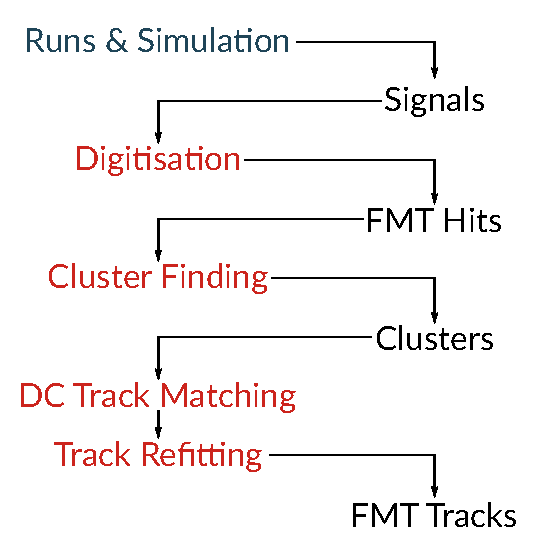
\includegraphics[width=\linewidth]{10fmt_recon.pdf}}
        \caption[FMT reconstruction summary]{FMT reconstruction summary.
        Data taking is coloured blue, data in black, and processes in red.
        Source: Own elaboration using \hyperlink{inkscape.org/}{Inkscape}.}
        \label{fig::12.11::fmt_reconstruction}
    \end{wrapfigure}

    The FMT is composed of six circular, flat detectors that cover angles ranging from $6$ to $29$ degrees.
    In its conception, it was anticipated that the FMT would improve the vertex resolution by a factor of 3 to 10 compared to the DC \cite{aune2009}.
    However, the currently implemented FMT deviates from the original design, with only three layers installed.
    This modification was necessitated by technical difficulties and concerns related to its Lorentz angle \cite{konczykowski2010}.

    Each of the three FMT layers is equipped with 1024 readout strips that exhibit a distinctive distribution, as depicted in the image on the right-hand side of Figure \ref{fig::12.10::fmt_geometry}.
    Additionally, the orientation of each layer differs by 60 degrees to ensure accurate measurements in the xy-plane, as illustrated in the image at the center of the same Figure \cite{acker2020mvt}.

    \begin{figure}[t]
        \centering\frame{
        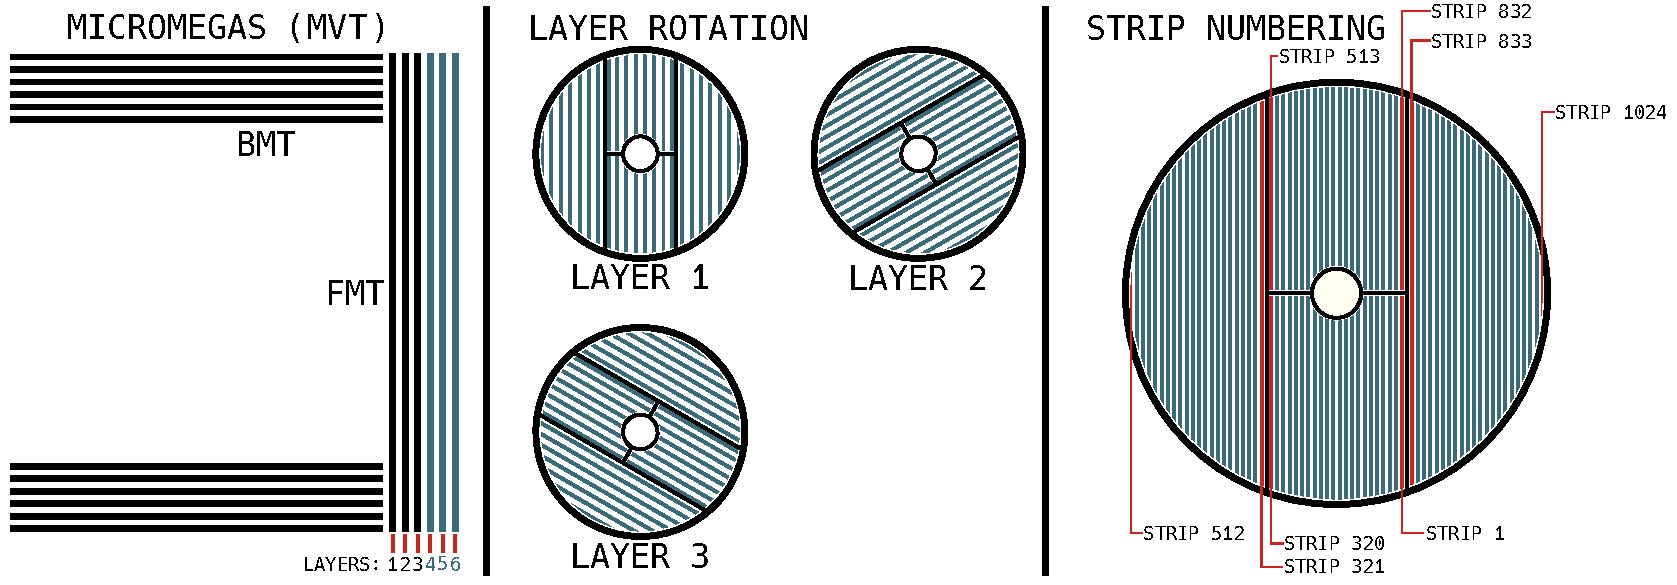
\includegraphics[width=\textwidth]{10fmt_geometry.pdf}}
        \caption[FMT detector geometry.]{FMT detector geometry. The first picture shows the distribution of the BMT and FMT layers, the second the different angle of each FMT layer, and the third the readout strip distribution of each FMT layer.
        Source: Own elaboration, using \hyperlink{inkscape.org/}{Inkscape}.}
        \label{fig::12.10::fmt_geometry}
    \end{figure}

    % !TEX root = ../main.tex
\subsubsection{FMT Track Reconstruction}
\label{sssec::fmt_track_reconstruction}
    Once a signal is detected on a readout strip and the data is stored, the information is extracted from it during offline reconstruction.
    The reconstruction process of the FMT closely resembles that of the DC.

    To begin with, when a signal is detected in a strip, it undergoes digitisation, processing, and is transformed into an \textbf{FMT Hit}.
    A set of FMT hits is then processed using a \textbf{Cluster Finding} algorithm, where a \textbf{Cluster} is defined as a group of hits that likely originate from the same particle track.
    Groups of clusters from different layers are subjected to a \textbf{DC Track Matching} algorithm, where they are matched to DC tracks generated by the DC Reconstruction process.
    Subsequently, a \textbf{Track Refitting} algorithm is employed for each DC track using the data from the clusters, resulting in updated tracks known as \textbf{FMT tracks}.
    An overview of this entire process is provided in Figure \ref{fig::fmt_recon}.


    % !TEX root = ../main.tex
\subsection{FMT Alignment}
\label{ssec::fmt_alignment}
% --+ Why is it needed +--------------------------------------------------------
    While in a perfect world the target and each detector would be installed precisely where they are needed, in the real world there is an unavoidable misalignment in their positions.
    This misalignment needs to be addressed and included into reconstruction:
    the software needs to be aware of where a detector is positioned in relation to the target to provide meaningful results.

    In the CLAS collaboration, the Calibration and Commissioning group (CalCom) is in charge of the alignment and calibration of each detector.
    Shifts and rotations that need to be applied for alignment are included in the Calibration and Conditions Database (CCDB), which is then read in reconstruction. % NOTE. A citation would be cool.

    The main goals of alignment work were three:
    First, to provide FMT alignment tables to Run Group F (RG-F) so that they may be used in reconstruction.
    Second, to check if the resolution improvement from FMT is good enough to justify the extra material added to the CLAS12 detector.
    Finally, to provide detailed information about these improvements so that Run Group E (RG-E) and other run groups can choose if they will include the detector to their runs.

% --+ Definitions +-------------------------------------------------------------
    Alignment shifts can be made in any of the three global axes:
    $z$, which is concentric to the beamline, $x$, which is parallel to the ground, and $y$, which points up from the ground.
    Then, alignment rotations can be done in any of these axes, and for the purposes of this work will be referred to as $\phi$ rotation (roll), when they're done around the $z$ axis, and pitch and yaw when they're done around the $x$ and $y$ axes respectively.

    To measure misalignment, we define a the Distance Of Closest Approach (DOCA) between a reconstructed DC track and an FMT cluster as a \textbf{Residual}.
    Due to each layer's geometry (refer to figure \ref{fig::fmt_geometry}), only the residuals in a layer's local $y$ axis (perpendicular to the strips) can be measured.
    This means that global $z$ and $\phi$ alignment can be done for each layer independently, but global $x$, global $y$, pitch, and yaw alignment has to be done for the entire detector at once.

% --+ How was it done +---------------------------------------------------------
    \begin{figure}[b!]
        \centering\frame{
        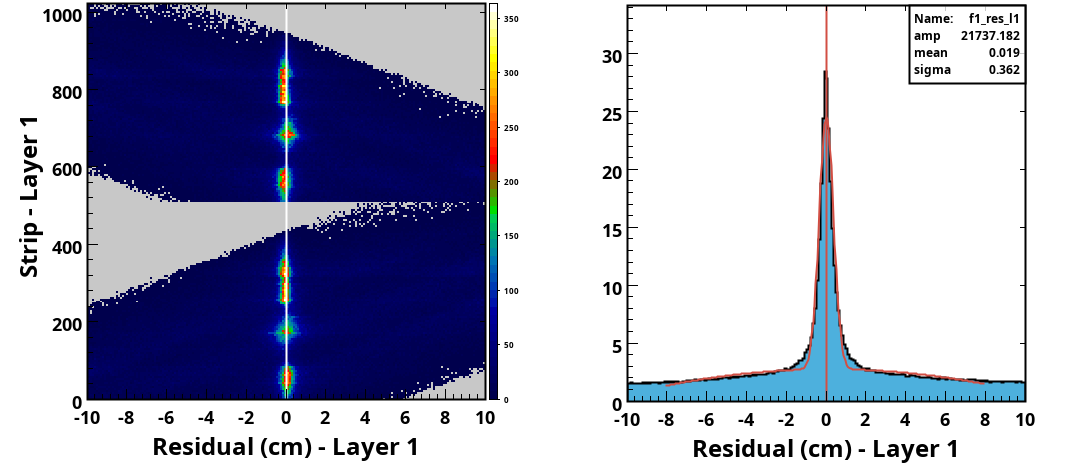
\includegraphics[width=\textwidth]{20res_example.png}}
        \caption[Example FMT residuals plot]{Example FMT residuals plot.
        Source: \hyperlink{github.com/JeffersonLab/clas12alignment}{CLAS12 alignment software}.}
        \label{fig::res_example}
    \end{figure}

    To minimise residuals, they are plotted for a particular shift or rotation in any of the relevant axes.
    An example of such a plot is shown in figure \ref{fig::res_example}.
    Since a Gaussian distribution is to be expected for the residuals, a Gaussian fit is applied to them.
    For $z$ and $\phi$ alignment, the goodness of a fit is evaluated heuristically by comparing their $\sigma$ and choosing the shift with the minimum $\sigma$.
    Then, for $x$, $y$, pitch, and yaw alignment, the goodness of a fit is evaluated heuristically by choosing the fit with the mean closest to $0$.
    The minimums are of course chosen within a healthy error margin.
    Examples of $z$ and $xy$ goodness of fit distributions can be seen in figure \ref{fig::resfit_example}.

    \begin{figure}[t!]
        \centering\frame{
        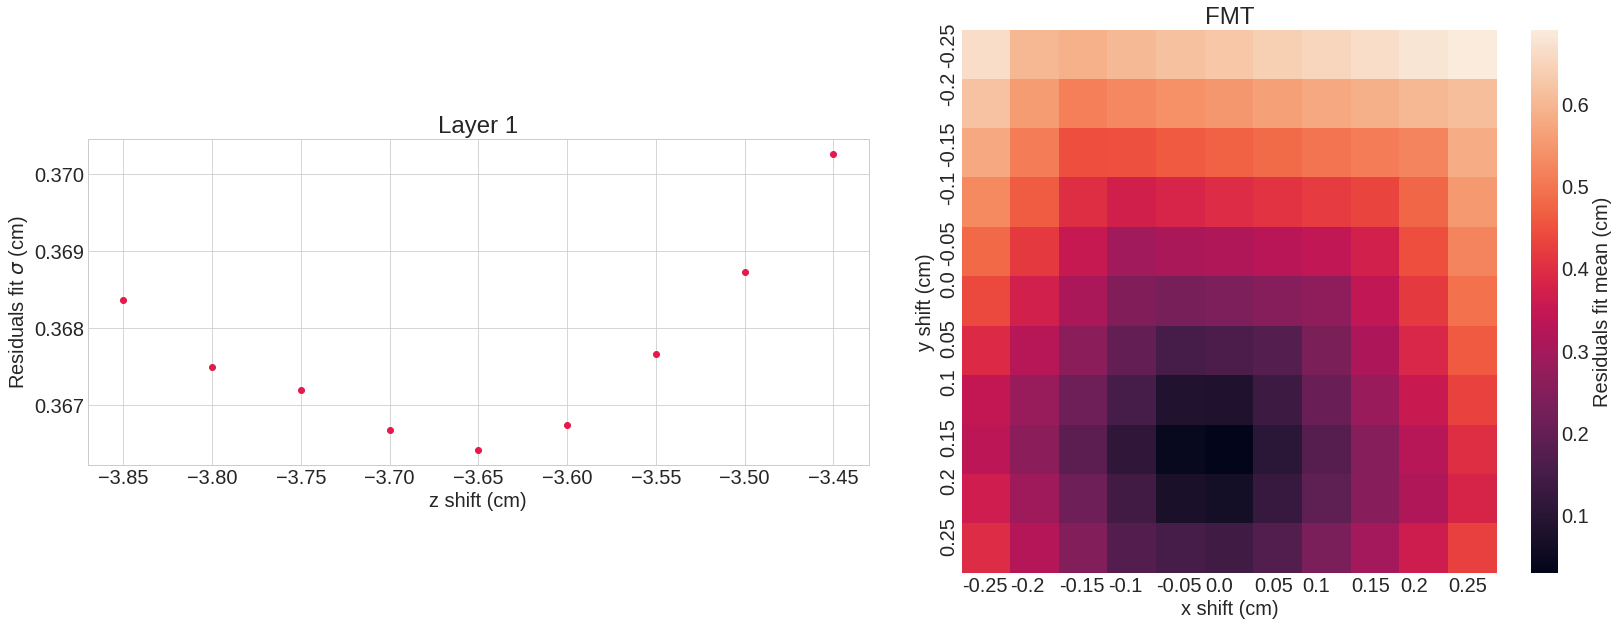
\includegraphics[width=\textwidth]{20resfit_example.png}}
        \caption[Examples of residuals goodness of fit plots]{Examples of residuals goodness of fit plots.
        Source: \hyperlink{github.com/JeffersonLab/clas12alignment}{CLAS12 alignment software}.}
        \label{fig::resfit_example}
    \end{figure}

% --+ Cuts +--------------------------------------------------------------------
\subsubsection{Fiducial Cuts}
    To reduce background, fiducial cuts are applied to the DC tracks and FMT clusters.
    This process is useful to increase data quality in order to obtain meaningful alignment results.

    For DC tracks, the cuts applied are:
    \begin{itemize}
        \item $\text{track}.z < \text{layer}.z$:
        Remove tracks with a vertex $z$ further downstream than the FMT layer before swimming.
        This is caused by reconstruction errors where the particle origin is outside of the target.
        % $9.84\%$ of tracks fail to meet this criterion in the sample data.
        \item $\mid\text{track}.z - \text{layer}.z\mid < 0.05 \text{cm}$:
        Remove tracks too far from the FMT layer after swimming.
        This was caused by bugs in the swimmer which will be mentioned in the next section.
        % $18.67\%$ tracks failed to meet this criterion.
        \item $5 \text{cm} < \sqrt{x^2 + y^2} < 25 \text{cm}$:
        Remove tracks outside of the layer's active region.
        % $35.22\%$ of the tracks were lost to this criterion.
        \item $\theta < ~66.42^{\circ}$:
        Remove tracks with a $\theta$ angle too high.
        When this happens, the same particle is affecting many strips, which causes the detector's data to not be as reliable as we want for alignment.
        % $7.22\%$ of tracks were lost to this criterion.
    \end{itemize}
    % From all these criteria, $70.95\%$ of the DC tracks were lost.
    % It is worth noting that after some reconstruction errors were fixed (as will be detailed in the following section), this percentage was reduced to $52.28\%$.

    For FMT clusters, the cuts applied are:
    \begin{itemize}
        \item $50 \text{ns} < \text{T}_{\text{min}} < 500 \text{ns}$:
        Cut clusters with an illogical $\text{T}_{\text{min}}$, which is the time of the first hit in the cluster.
        % $21.12\%$ of clusters fail to meet this criterion.
        \item $\text{size} > 1$ $\&\&$ $\text{E} > 100$:
        Cut small clusters with high energy, which are generally considered bad.
        % Only $7.36\%$ clusters are lost to this criterion.
        \item $\text{size} < 5$:
        Cut large clusters, which are not considered very useful.
        % Only $7.77\%$ are lost to this criterion.
    \end{itemize}
    % From all these criteria, $36.25\%$ of the FMT clusters were lost.

% --+ Minimisation of residuals +-----------------------------------------------
\subsubsection{Residuals Improvements}
    To validate the alignment algorithm proposed, it was tested on RG-F data (run $\mathbf{11983}$).
    The improvement in residuals is immediately obvious, as can be seen in figure \ref{fig::res_comparison}, noting the difference in scale between the top and bottom plots.

    \begin{figure}[t!]
        \centering\frame{
        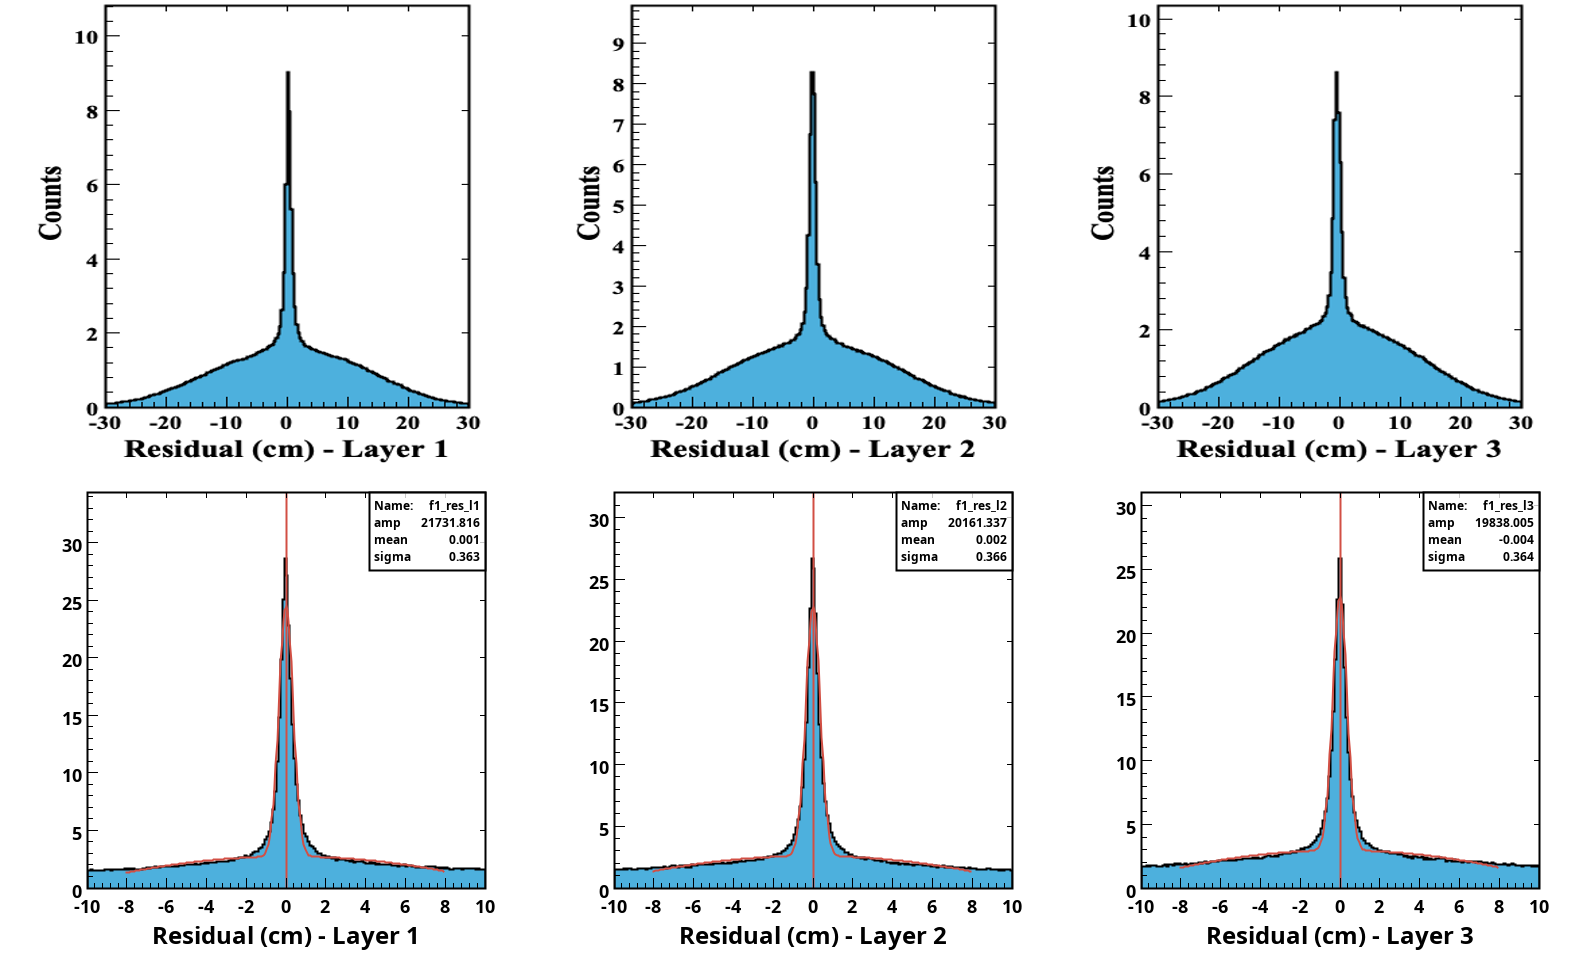
\includegraphics[width=\textwidth]{20res_comparison.png}}
        \caption[Residuals distribution improvement.]{Residuals distribution before (upper image) and after (lower image) alignment.
        Source: \hyperlink{github.com/JeffersonLab/clas12alignment}{CLAS12 alignment software}.}
        \label{fig::res_comparison}
    \end{figure}

    As can be seen in the figure, the $z$ and $\phi$ alignment heavily reduces the background, increasing the number of residuals near the mean of the distribution.
    In addition, the $x$ and $y$ alignment pushes this mean to zero, whereas it was slightly off before.
    Finally, no meaningful results were obtained for pitch and yaw alignment.
    This is attributed to how small the rotations around the $x$ and $y$ axes are, compounded with the fact that three layers do not provide enough data to perform alignment precise enough.

    To measure the mean and $\sigma$ of the distribution, a Gaussian fit was used.
    Its parameters are

     \begin{align*}
        \Big( \text{amp} \cdot \text{gaus}(\mu, \sigma) \Big) &+ \Big( p_0 + p_1\cdot x + p_2\cdot x^2 \Big) \\
        \text{gaussian} \hspace{0.8cm} &+ \hspace{1cm} \text{background}
    \end{align*}

    The results obtained are included in the CCDB at:

    \small\href{clasweb.jlab.org/cgi-bin/ccdb/versions?table=/geometry/fmt/alignment}{\texttt{clasweb.jlab.org/cgi-bin/ccdb/versions?table=/geometry/fmt/alignment}}

    Alignment was also later performed for Run Group M (RG-M) data successfully, proving that the alignment procedure is agnostic to a particular run.
    How this alignment procedure affects the resolution of the entire CLAS12 detector will be explored at the end of the chapter.

    The procedure described in this section is documented and shared publicly.
    It can be seen at:

    \href{github.com/JeffersonLab/clas12alignment/tree/master/fmt}{\texttt{github.com/JeffersonLab/clas12alignment/tree/master/fmt}}

    % !TEX root = ../main.tex
\subsection{FMT Reconstruction Work}
\label{ssec::fmt_reconstruction_work}
% --+ Why is it needed +--------------------------------------------------------
    As the work on FMT alignment progressed, certain modifications were required in FMT reconstruction.
    These modifications primarily involved incorporating the alignment shifts determined during the alignment process into the reconstruction.
    Additionally, some fixes were made to address issues that were identified during the alignment work.
    These changes ensure that the reconstruction process takes into account the alignment information and addresses any related issues that were encountered.

% --+ What was done +-----------------------------------------------------------
    First, the loading of shifts from the CCDB was included in the standard geometry class of the FMT reconstruction package.
    Then, standard methods to include the shifts in any frame of reference change were implemented.
    Finally, the code was studied in detail, and the shifts were added in all instances where they were required since the package originally didn't consider their application.

    ``Crossmaking'' is the process of matching clusters in different layers to obtain an accurate 3D estimate of the position of a track \cite{ziegler2020}.
    This process was initially included in FMT reconstruction to facilitate the reconstruction for the six FMT layers.
    However, as mentioned before, only three FMT layers were installed for the RG-F run, and future runs may also use three layers due to concerns with the Lorentz angle when using six layers.
    To simplify the reconstruction process and make better use of the available number of layers, crossmaking was removed from the reconstruction.

    Outside of FMT reconstruction, some minor changes were also required in the DC reconstruction package since some of its components depend on the FMT layers' positions.
    Additionally, the swim package diagnostic was updated as it failed to properly reconstruct the positions of tracks near the FMT layers.

% --+ Juicy link +--------------------------------------------------------------
    A detailed list of the updates applied can be found in the following pull request to the \texttt{clas12-offline-software} repository:

    \href{github.com/JeffersonLab/clas12-offline-software/pull/726}{\texttt{github.com/JeffersonLab/clas12-offline-software/pull/726}}.

    % !TEX root = ../main.tex
\subsection{Validation and Results}
\label{12.40::validation_and_results}
% --+ Data used +---------------------------------------------------------------
    Just like the residuals validation, the results presented in this document are based on the application of this work to RG-F data.
    It is important to note that the RG-F target is approximately 55 centimetres long, which is much larger than the average CLAS12 target \cite{hattawy2019}.
    Specifically, the runs used for testing and validation are presented in Table \ref{tab::12.40::rgf_data}, and the run used to obtain the data displayed in this section was 011983.

    \begin{table}[h!]
        \centering
        \begin{tabular}{lllll}
            \toprule
            \textbf{Run Number} & \textbf{Energy (MeV)} & \textbf{Current (nA)} & \textbf{Configuration} & \textbf{Target} \\
            \midrule \midrule
            011983              & 10389.4               &  50                   & Inbending              & D2 \\
            012016              & 10389.4               & 250                   & Inbending              & D2 \\
            012439              &  2186.4               &  15                   & Inbending              & H2 \\
            012461              & 10196.6               &  20                   & Inbending              & D2 \\
            \bottomrule
        \end{tabular}

        \caption{RG-F runs used for validation.}
        \label{tab::12.40::rgf_data}
    \end{table}

    % !TEX root = ../main.tex
\subsubsection{Cuts}
\label{12.41::cuts}
    \begin{figure}[b!]
        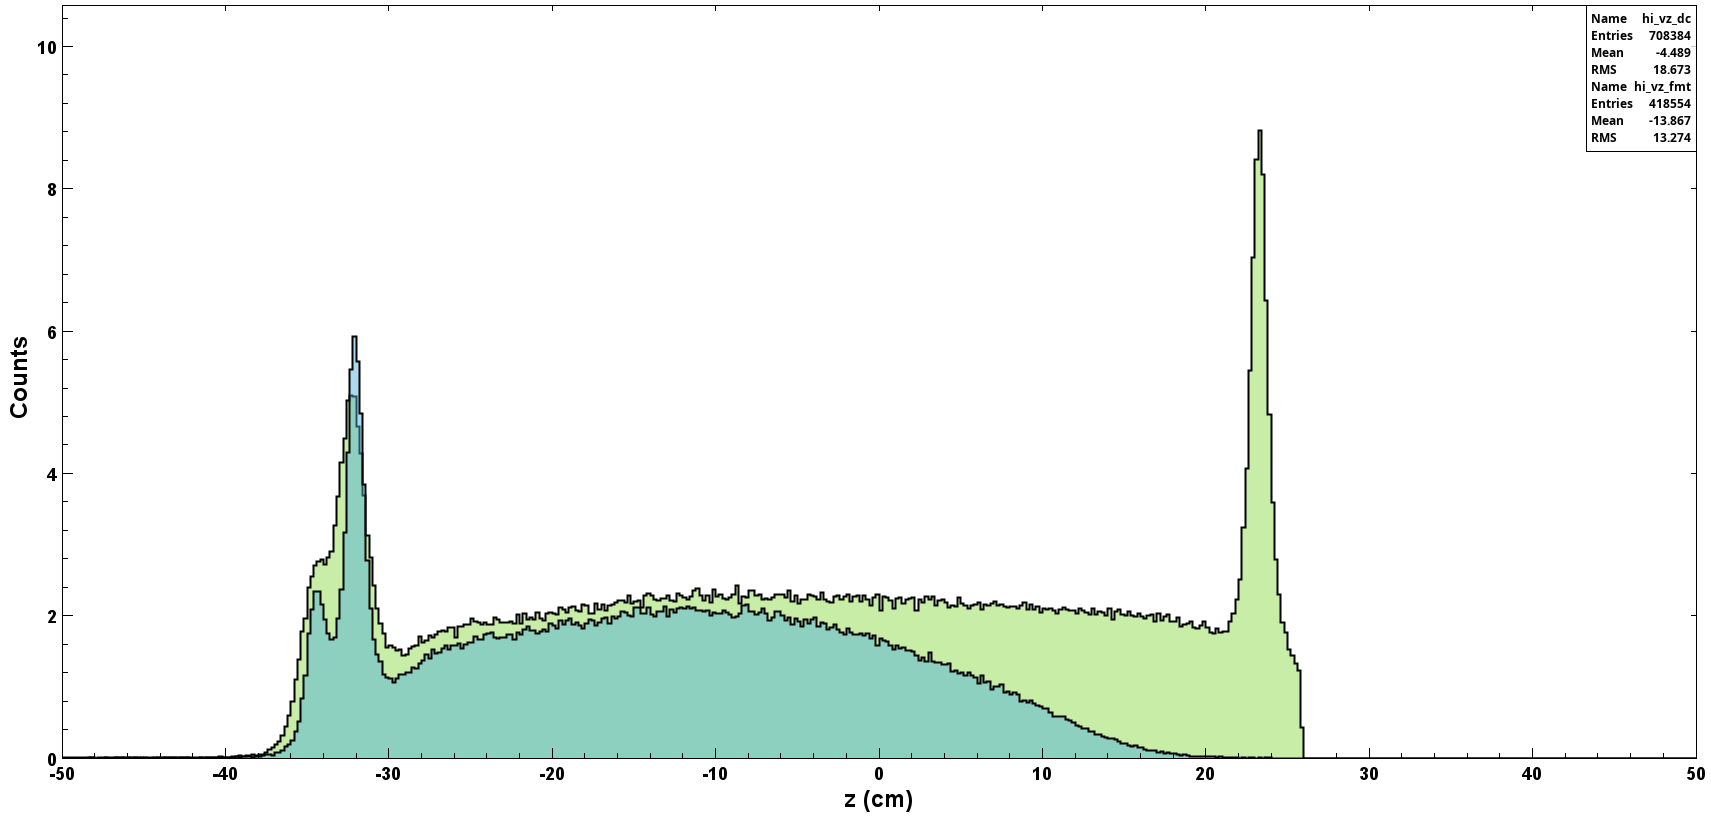
\includegraphics[width=\textwidth]{41dc_vs_fmt.png}
        \caption[DC vs. FMT $z$ without geometric correction]
        {DC vs. FMT vertex $z$ for electrons without any geometric correction.
        DC tracks are shown in green while FMT tracks are shown in blue.
        Note that the dark cyan colour comes from the overlap.}
        \floatfoot{Source: Own elaboration, using the \texttt{fmtVertex.groovy} script in \href{https://github.com/JeffersonLab/clas12alignment}{CLAS12 alignment software}.}
        \label{fig::12.41::dc_vs_fmt_vz_11983}
    \end{figure}

    Some additional cuts are applied to the tracks to obtain the plots presented in this section.
    These cuts are used to remove very poor tracks that would not be suitable for analysis regardless.
    The applied cuts are as follows:
    \begin{itemize}
        \item
            \texttt{abs(chi2pid) < 5}:
            This cut removes tracks that do not provide sufficient certainty regarding the particle's PID.
        \item
            \texttt{vz < fmtZ}:
            This cut removes tracks located further downstream than the FMT.
        \item
            \texttt{chi2/ndf < 15}:
            This cut excludes tracks with excessively high uncertainty.
    \end{itemize}

    % !TEX root = ../main.tex
\subsubsection{Geometry Effect}
\label{12.42::geometry_effect}
    To evaluate the enhancement in vertex resolution, we will compare the vertex positions of tracks that underwent only DC reconstruction with those that underwent both DC and FMT reconstruction.
    For convenience, we will refer to the former as DC tracks and the latter as FMT tracks.
    Considering that the $z$ axis is aligned with the beamline, Figure \ref{fig::12.41::dc_vs_fmt_vz_11983} illustrates the $z$ positions of the vertex for DC tracks versus FMT tracks.

    To comprehend the plot in Figure \ref{fig::12.41::dc_vs_fmt_vz_11983}, it is valuable to examine the RG-F target.
    The target consists of a large gas-filled chamber with a varying composition across different runs.
    The distance between the chamber windows measures $553.32$ millimetres.
    Furthermore, it was observed that the upstream window of the target is positioned approximately $24$ millimetres away from the beam window.
    All windows are constructed from aluminium and have a thickness of $15$ micrometers.
    A detailed depiction of the target can be found in Addendum 1.

    Based on Figure \ref{fig::12.41::dc_vs_fmt_vz_11983}, it is evident that the FMT detector solely detects the upstream windows, completely overlooking the downstream one.
    This issue stems from a geometric constraint: the downstream window falls outside the active detection area of the FMT.
    This effect is clearly illustrated in Figure \ref{eq::12.42::vz_vs_theta}, where the $\theta$ angle is plotted against the vertex $z$ coordinate.
    The two red lines in the plots represent the FMT's active area, and it is apparent that the downstream window lies outside this region, thereby explaining its absence.

    \begin{figure}[t!]
        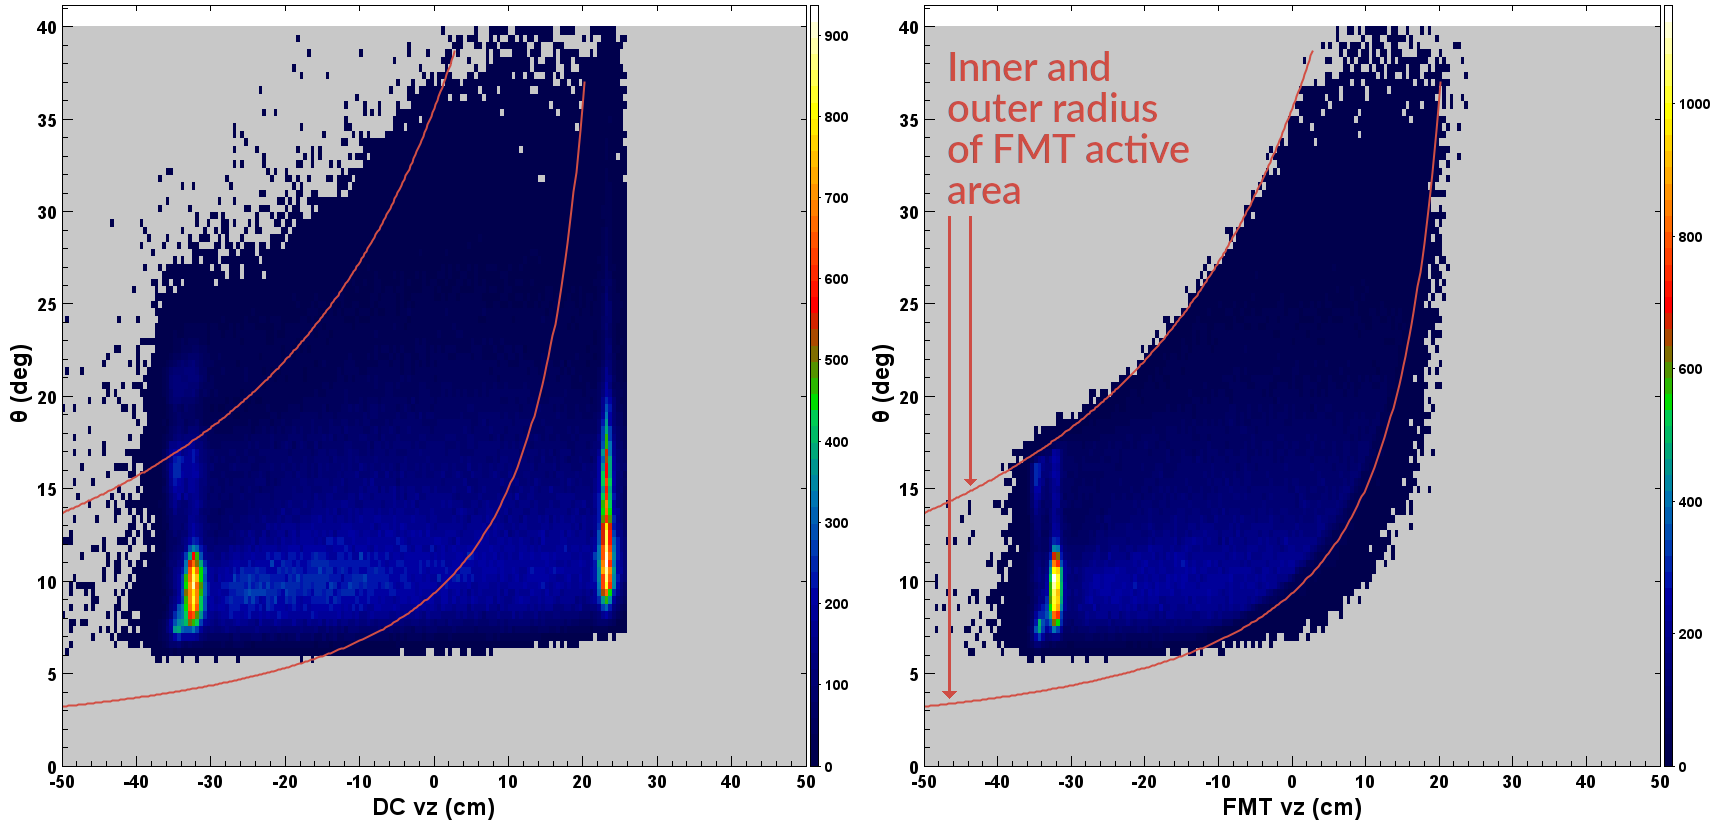
\includegraphics[scale=0.24]{42theta_dc_vs_fmt.png}
        \caption[$z$ vs. $\theta$ for DC and FMT]
        {$z$ vs. $\theta$ for DC and FMT for electrons without any geometry correction.
        FMT's active area are shown in red lines.}
        \floatfoot{Source: Own elaboration, using the \texttt{fmtVertex.groovy} script in \href{https://github.com/JeffersonLab/clas12alignment}{CLAS12 alignment software}.}
        \label{eq::12.42::vz_vs_theta}
    \end{figure}

    To compensate for this geometric effect, we introduce an additional cut based on the plotted curves.
    The curves can be described by the following equations
    \begin{equation}
        c_1(z) = 57.29 \cdot \arctan\left(\frac{r_\text{inner}}{z_0 - z}\right),
        \hspace{0.5cm}
        c_2(z) = 57.29 \cdot \arctan\left(\frac{r_\text{outer}}{z_0 - z}\right).
        \label{eq::12.42::fmt_geometry_cut}
    \end{equation}

    Here, $r_\text{inner}$ represents the radius of the hole at the center of the FMT, $r_\text{outer}$ denotes the radius of the outer circumference of the FMT, and $z_0$ corresponds to the $z$ position of the first FMT layer plus the drift distance.
    All these parameters are obtained from the CCDB.

    % !TEX root = ../main.tex
\subsubsection{Vertex Resolution Improvement}
\label{12.43::vertex_resolution_improvement}

    \begin{figure}[b!]
        \frame{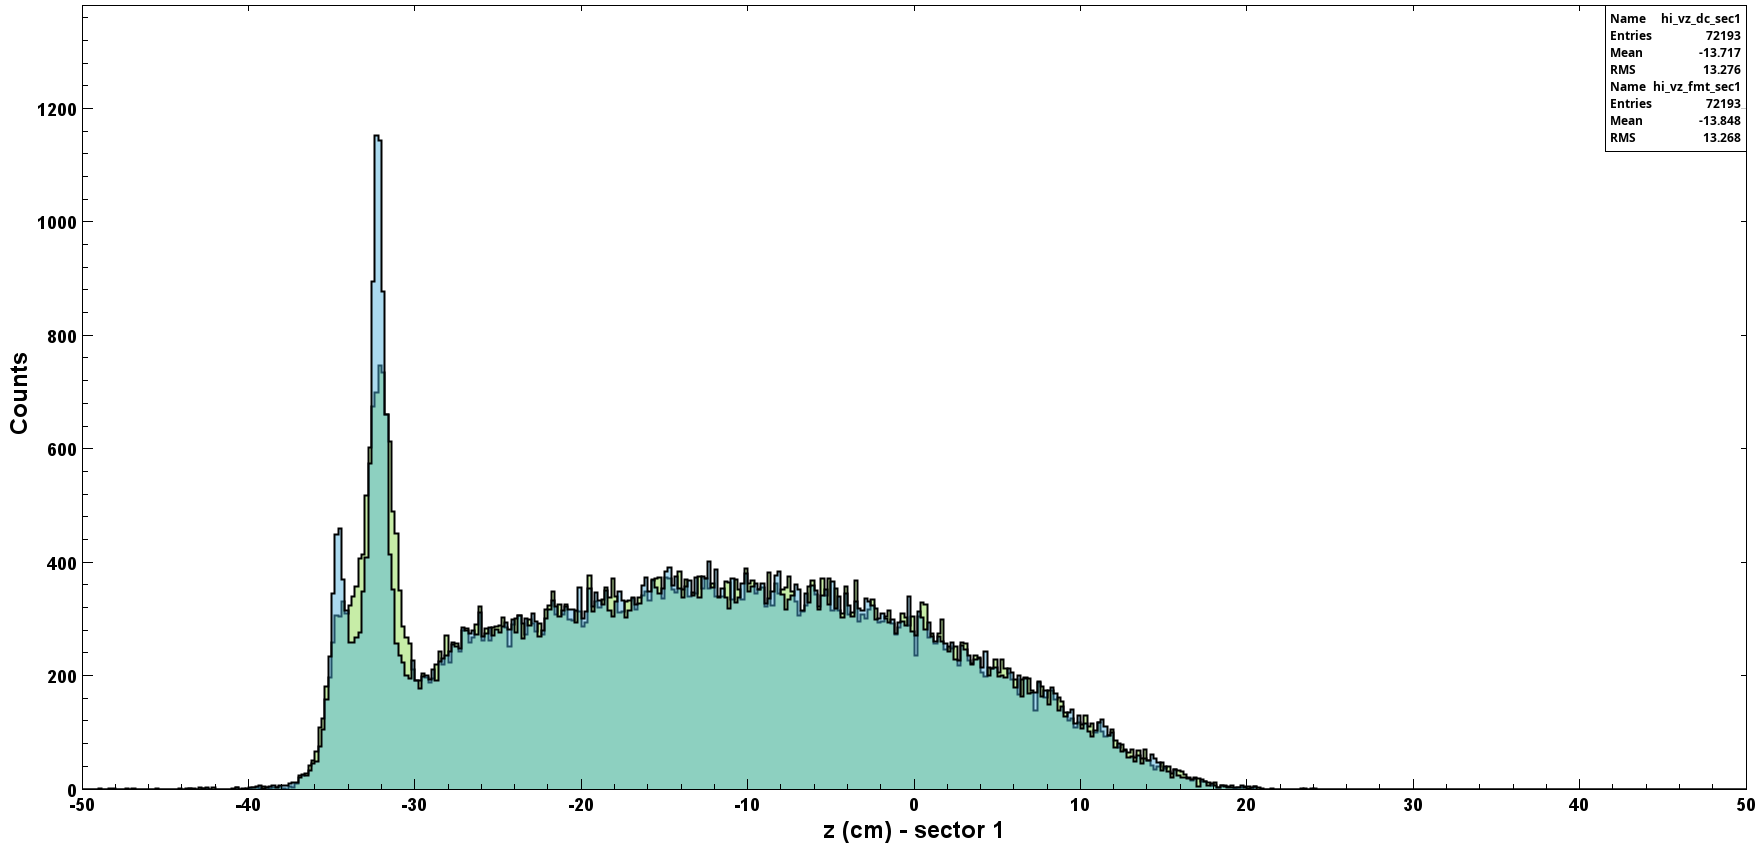
\includegraphics[scale=0.24]{40dc_vs_fmt_sector1.png}}
        \caption[DC vs FMT $z$ with geometry correction]
        {DC vs FMT vertex $z$ for electrons with a geometric correction.
        DC tracks are shown in green while FMT tracks are shown in blue.
        Data from only one CLAS12 sector was used to obtain this plot.}
        \floatfoot{Source: Own elaboration, using the \texttt{fmtVertex.groovy} script in \href{https://github.com/JeffersonLab/clas12alignment}{CLAS12 alignment software}.}
        \label{fig::12.43::dc_vs_fmt_vz_11983_corrected}
    \end{figure}

    Furthermore, an additional cut has been introduced.
    As of the FMT alignment work, beam alignment for RG-F data had not been carried out, resulting in a decrease in vertex resolution.
    To mitigate the impact of this alignment issue on reconstruction accuracy, we have implemented a cut to utilise only one sector of the detector.

    The resolution plot, comparing DC and FMT tracks after applying all the previously mentioned cuts, is depicted in Figure \ref{fig::12.43::dc_vs_fmt_vz_11983_corrected}.
    To evaluate the resolution for both DC and FMT tracks, we utilise a fit consisting of two Gaussian curves combined with a quadratic curve to account for the background.
    The fit is defined as follows
    \begin{equation*}
        \text{amp}_1 \cdot \text{gaus}(z, z_\text{max}, \sigma) + \text{amp}_2 \cdot \text{gaus}(z, z_\text{max} - 2.4, \sigma) + p_1 + p_2\cdot z + p_3\cdot z^2,
    \end{equation*}
    where
    \begin{itemize}
        \item
            $\text{amp}1$ represents the amplitude of the largest peak, and $z\text{max}$ corresponds to its $z$ position,
        \item
            $\text{amp}_2$ signifies the amplitude of the leftward peak, which has been measured to be at a position of $2.4$ centimetres, and
        \item
            the remaining parameters, $p_1$, $p_2$, and $p_3$, are obtained through the fitting process.
    \end{itemize}

% --+ Resolution for electrons +------------------------------------------------
    For electrons in run 011983 (low luminosity, 50 nA), the analysis yields a DC resolution of $\sigma_\text{DC} = 0.875$ cm and an FMT resolution of $\sigma_\text{FMT} = 0.387$ cm.
    This indicates a doubling of the resolution achieved with the inclusion of the FMT detector.

    Similarly, for electrons in run 012016 (production luminosity, $250$ nA), the analysis shows a DC resolution of $\sigma_\text{DC} = 1.009$ cm and an FMT resolution of $\sigma_\text{FMT} = 0.596$ cm.

    % !TEX root = ../main.tex
\subsubsection{Conclusions}
\label{12.44::conclusions}
    Although the improvement in resolution is not as significant as initially anticipated for the detector, it remains an encouraging result.
    The enhanced resolution enables more precise measurements of the target position.
    As a practical implication, it allows for double targets to be positioned closer to each other, thereby benefiting the derived physics from experiments like the RG-E run.

    The reason for the smaller-than-predicted improvement in resolution can be attributed to the initial projection, which assumed the presence of six FMT layers.
    The inclusion of six layers would provide additional positional data along the particle's track, thereby enhancing the accuracy of the vertex position measurement during the fitting process.

% --+ Why no improvements is seen on vertex momentum resolution +---------------
    Furthermore, due to the limited number of layers and their close proximity in the FMT detector, it exhibits a small lever arm.
    As a result, the detector's contribution to the vertex momentum resolution is not significant, as it does not provide sufficient additional data to accurately determine the track's momentum.

% --+ Show detector efficiency +------------------------------------------------
    In order to gain a better understanding of the FMT detector, we conducted a brief study on its efficiency.
    The efficiency is defined as the ratio of the number of FMT tracks to the number of DC tracks, representing how many of the DC tracks were also detected by the FMT.

    For the three-layer configuration, the efficiency is approximately $88.96\%$.
    Figure \ref{fig::12.44::fmt_azimuthal_efficiency} illustrates the layer-by-layer efficiency, showing no anomalous geometric effects.
    The observed gaps in efficiency are solely a result of the CLAS12 detector's geometry, which is divided into six sectors.

    \begin{figure}[b]
        \centering\frame{
        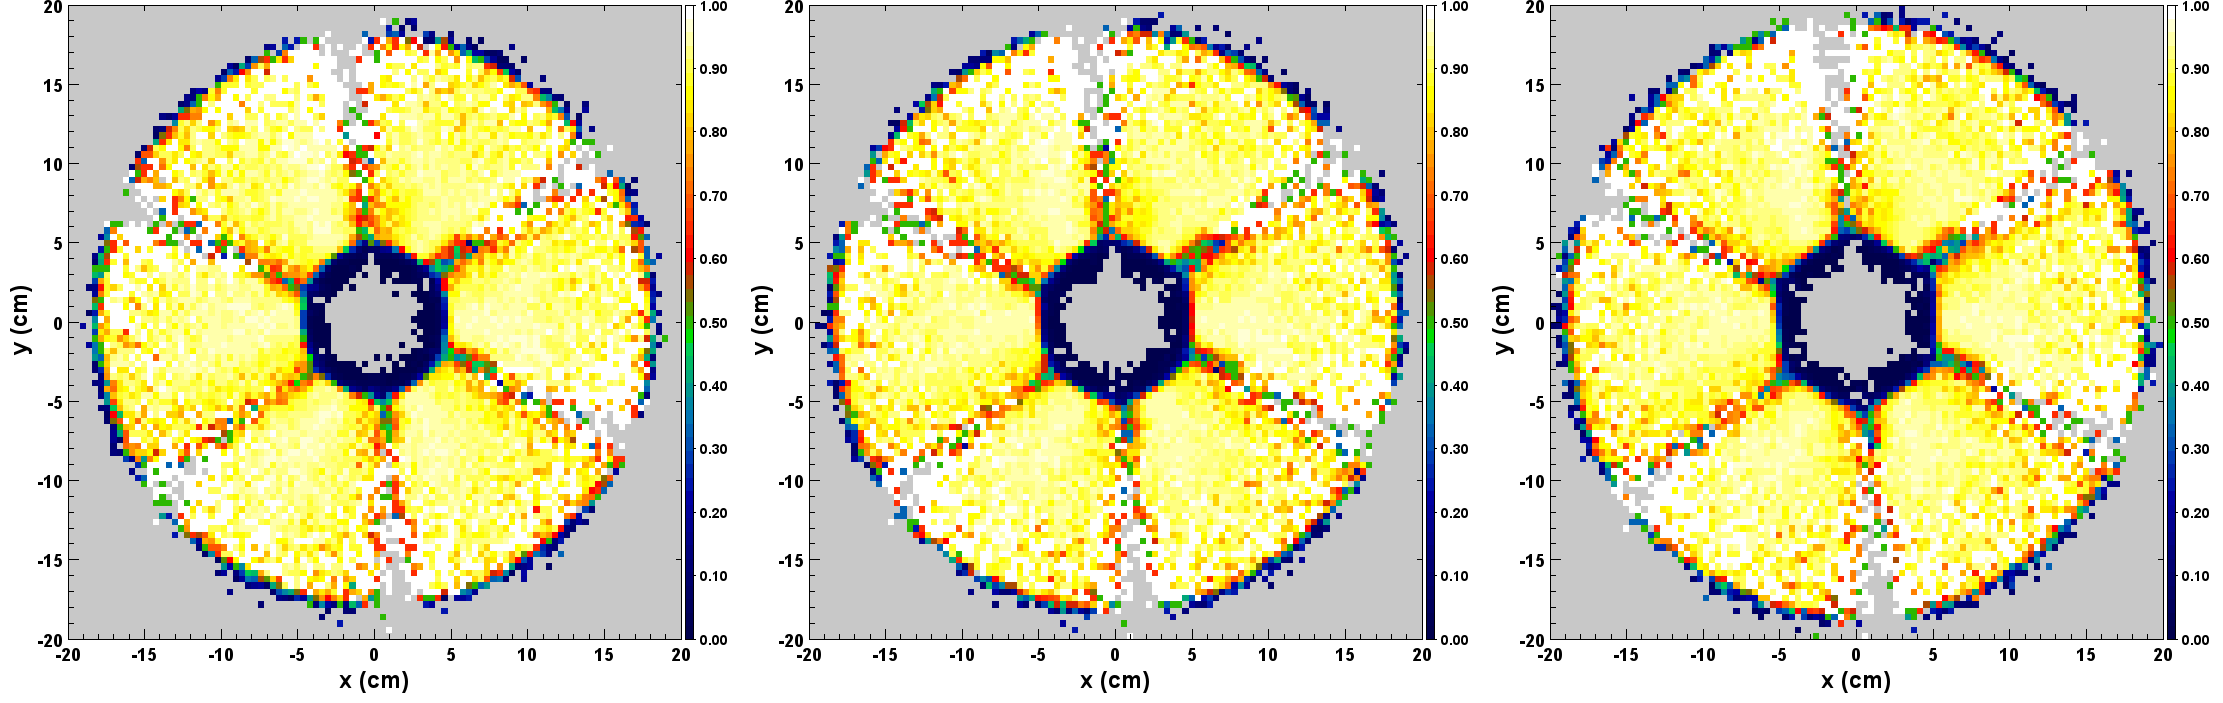
\includegraphics[width=\textwidth]{44fmt_efficiency.png}}
        \caption[FMT layers efficiency]{Efficiency of each FMT layer.
        Source: \texttt{fmtVertex.groovy} script in \hyperlink{github.com/JeffersonLab/clas12alignment}{CLAS12 alignment software}.}
        \label{fig::12.44::fmt_azimuthal_efficiency}
    \end{figure}



    \pagebreak

    % --+ Data Analysis +-------------------------------------------------------
    \graphicspath{{13data_analysis/img}}
    % !TEX root = ../main.tex
\section{Data Analysis}
\label{sec::dataanalysis}
    The first section on this chapter describes a C program developed by the author to perform the analysis in this thesis.
    Then, the second section talks about the Deep Inelastic Scattering (DIS) kinematics which define the cuts made to the data.
    The third section goes into detail about the approach to include sampling fraction to the analysis.
    Finally, the last section describes the simulations produced and the acceptance study made based on these.

    % !TEX root = ../main.tex
\subsection{\texttt{clas12-rge-analysis}}
\label{13.10::clas12_rge_analysis}
    To perform the acceptance analysis reported in this thesis, the author developed an extensive C/C++ program that runs on the ROOT library.
    The purpose of this program is not only to conduct the analysis described in this thesis but also to be used for RG-E analysis in general.
    The program and its source code are freely available under the GNU LGPLv3 license and can be accessed on GitHub at: \href{https://github.com/bleaktwig/clas12-rge-analysis}{github.com/bleaktwig/clas12-rge-analysis}.
    Issues and pull requests are welcomed, as they are crucial for maintaining the program and facilitating collaborative development in the repository.

    After compiling the program using \texttt{make}, five executables are obtained in the \texttt{bin} directory.
    The following sections provide a description of each executable.

    % !TEX root = ../main.tex
\subsubsection{\texttt{hipo2root}}
\label{sssec::hipo2root}
    CLAS12 reconstruction uses a custom data file named High-Performance Input Output (HIPO) format, developed by Gagik Gavalian \cite{chekanov2021}.
    The CLAS collaboration provides a set of tools to work with this format, allowing to read, write, and draw plots from HIPO files.
    Despite this, however, users at RG-E are much more familiar with the traditional ROOT files, and thus a conversion tool was developed.

    \texttt{hipo2root} filters through a HIPO file's data, and creates a ROOT file with pre-selected sections of storage, called banks.
    The selection of banks is based on data that is useful to RG-E analysis, and a user can easily add additional banks by editing the program's source files.
    The output of the executable is a ROOT file containing the selected banks as trees, a standard ROOT array-like variable.

    It's manual entry is:
    \begin{lstlisting}
Usage: hipo2root [-hfn:w:] infile
 * -h         : show this message and exit.
 * -f         : set this to true to process FMT::Tracks bank. If this is set
                and FMT::Tracks bank is not present in the HIPO file, the
                program will crash.
 * -n nevents : number of events.
 * -w workdir : location where output root files are to be stored. Default
                is root_io.
 * infile     : input HIPO file. Expected format is <text>run_no.hipo.

Convert a file from hipo to root format. This program only conserves the banks that are useful for RG-E analysis, as specified in the `lib/rge_hipo_bank.h` file. It's important for the input hipo file to specify the run number at the end of the filename (`<text>run_no.hipo`), so that `hipo2root` can get the beam energy from the run number.

Since simulation files don't have a run number, we use a convention for specifying the beam energy. For this files, the filename should be `<text>999XXX.hipo`, where `XXX` is the beam energy used in the simulation in [0.1*GeV].
    \end{lstlisting}

    % !TEX root = ../main.tex
\subsubsection{\texttt{extract\_sf}}
\label{sssec::extract_sf}
    Some analysis from CLAS12 is needed to obtain the sampling fraction of the detector's calorimeters.
    This is done by the \texttt{extract\_sf} executable, which uses the particles' momenta and deposited energy.
    The exact methodology and results obtained are discussed in section \ref{ssec::sampling_fraction}.

    The manual entry of the program is:
    \begin{lstlisting}
Usage: extract_sf [-hn:w:d:] infile
 * -h         : show this message and exit.
 * -n nevents : number of events
 * -w workdir : location where output root files are to be stored. Default
                is root_io.
 * -d datadir : location where sampling fraction files are stored. Default
                is data.
 * infile     : input ROOT file. Expected file format: <text>run_no.root.

Obtain the EC sampling fraction from an input file. An alternative to using this program is to fill the output file corresponding to the studied run (by default stored in the `data` directory) with the data obtained from [CCDB](https://clasweb.jlab.org/cgi-bin/ccdb/versions?table=/calibration/eb/electron_sf). The function used to fit the data is

[0]*Gaus(x,[1],[2]) + [3]*x*x + [4]*x + [5]

where *[0]* is the amplitude of the Gaussian, *[1]* and *[2]* its mean and sigma, and *[3]*, *[4]*, and *[5]* the *p0*, *p1*, and *p2* used to fit the background.

The output of the program is the `sf_params_<run_no>.txt`, which contains a table with the sampling fractions and their errors. The table is formatted like the one at CCDB, as in

         | sf0     sf1     sf2     sf3     sfs1    sfs2    sfs3    sfs4
---------+-----------------------------------------------------------------
sector 1 | %011.8f %011.8f %011.8f %011.8f %011.8f %011.8f %011.8f %011.8f
sector 2 | %011.8f %011.8f %011.8f %011.8f %011.8f %011.8f %011.8f %011.8f
sector 3 | %011.8f %011.8f %011.8f %011.8f %011.8f %011.8f %011.8f %011.8f
sector 4 | %011.8f %011.8f %011.8f %011.8f %011.8f %011.8f %011.8f %011.8f
sector 5 | %011.8f %011.8f %011.8f %011.8f %011.8f %011.8f %011.8f %011.8f
sector 6 | %011.8f %011.8f %011.8f %011.8f %011.8f %011.8f %011.8f %011.8f
    \end{lstlisting}

    % !TEX root = ../main.tex
\subsubsection{\texttt{acc\_corr}}
\label{sssec::acc_corr}
    The \texttt{acc\_corr} executable is used to count the number of thrown and simulated events from two different ROOT files.
    Based on the program's input, it separates the data into appropriate 5-dimensional bins, counts the entries for all available particles in the generated file, and exports the results into a text file.
    The results and plots presented in section \ref{ssec::acceptance_correction} were generated using the data obtained from this program.

    The manual entry of the program is:
    \begin{lstlisting}
Usage: acc_corr [-hq:n:z:p:f:g:s:d:FD]
 * -h         : show this message and exit.
 * -q ...     : Q2 bins.
 * -n ...     : nu bins.
 * -z ...     : z_h bins.
 * -p ...     : Pt2 bins.
 * -f ...     : phi_PQ bins (in degrees).
 * -g genfile : generated events ROOT file.
 * -s simfile : simulated events ROOT file.
 * -d datadir : location where sampling fraction files are found.
                Default is data.
 * -F         : flag to tell program to use FMT data instead of DC data
                from the simulation file.
 * -D         : flag to tell program that generated events are in
                degrees instead of radians.

Get the 5-dimensional acceptance correction factors for *Q2*, *nu*, *z_h*, *Pt2*, and *phi_PQ*. For each optional argument, an array of doubles is expected. The first double will be the lower limit of the leftmost bin, the final double will be the upper limit of the rightmost bin, and all doubles between them will be the separators between each bin.

The output will be written to the `acc_corr.txt` file, by default in the `data` directory, which is formatted to make it easy to read by the `draw_plots` program:
* First line contains five integers; the size of each of the five binnings.
* The next five lines are each of the binning schemes, in order *Q2*, *nu*, *z_h*, *Pt2*, and *phi_PQ*.
* The following line contains one integer which is the size of the list of PIDs, followed by a line containing each of these PIDs.
* Finally, a number of lines equal to the number of PIDs follows. Each line contains a list of the bins, ordered as `[Q2][nu][z_h][Pt2][phi_PQ]`.
    \end{lstlisting}

    % !TEX root = ../main.tex
\subsubsection{\texttt{make\_ntuples}}
\label{13.14::make_ntuples}
    This executable operates on one or more files generated by \texttt{hipo2root} and produces a ROOT file that contains a set of \texttt{ntuples} relevant to the analysis.
    Furthermore, based on the specific requirements of this thesis' analysis, the executable generates two sets of \texttt{ntuples}.
    Both sets have the same \texttt{ntuple} format, but the former utilises only DC tracking data while the latter incorporates both DC and FMT tracking data.

    \begin{table}[b]
        \begin{tabularx}{240pt}{Xllllll}
            \multicolumn{7}{c}{\textit{Particle Identification Truth}} \\
            \toprule
                     & $e$      & $\pi$ & $K$  & $p$  & $n$  & $\gamma$ \\
            \midrule
            $e$      & 1.00     &       &      &      &      &          \\
            $\pi$    &          & 1.00  & 0.09 & 0.02 &      &          \\
            $K$      &          &       & 0.91 &      &      &          \\
            $p$      &          &       &      & 0.98 &      &          \\
            $n$      &          &       &      &      & 1.00 &          \\
            $\gamma$ &          &       &      &      &      & 1.00     \\
            \bottomrule
        \end{tabularx}
        \caption[Particle identification matrix for the FD]
        {Particle identification matrix for the FD.
        The rows show the PID assigned by reconstruction while the columns the one assigned by the \texttt{make\_ntuples} program.
        The diagonal elements are correctly identified, while the off-diagonal elements are misidentified.}
        \label{tab::13.14::make_ntuples_pid}
    \end{table}

    For each event, the program executes the following algorithm:

    \begin{enumerate}
        \item
            First, the program identifies the TOF of the trigger electron.
            The hits of the trigger electron in the FD scintillators and FD calorimeters are listed in order of priority based on the precision of each detector's TOF measurement.
            The detectors are prioritised as follows: FTOF panel-1b, FTOF panel-1a, FTOF panel-2, PCAL, ECIN, and ECOU, as described in Section \ref{11.210::forward_detector}.
            Next, the program iterates over the list of hits, extracting the TOF value from the earliest hit in the most precise available layer.

        \item
            Next, for each available track, two particle objects are instantiated.
            These objects contain the relevant data for the particle, including its vertex position, vertex momentum, charge, beta, and the CLAS12 sector through which it passed.
            The first object corresponds to the tracking data obtained from the DC, while the second object incorporates both the DC and the FMT tracking data.
            The assignment of the particle's PID will be carried out later in the process.

        \item
            The program computes and stores the particle's deposited energy in the calorimeters.
            This involves summing up the energy deposited by all the hits associated with the particle's track for each calorimeter.

        \item
            The program counts the number of produced photoelectrons in the HTCC and LTCC for the particle.
            Furthermore, the particle's TOF is computed using the same procedure as the one employed for the trigger electron's TOF, considering the hits in the detectors prioritised by their precision.

        \item
            The program assigns the Particle Identification PID to the particle.
            The process is very similar to the PID assignment in reconstruction, as described in Section \ref{11.230::offline_reconstruction}.
            However, the assigned PID is not directly used in order to allow users to modify parameters and define new criteria for the PID assignment.

            Although this process typically yields the same results as reconstruction, there is a slight error in the PID assignment.
            This error is presented in Table \ref{tab::13.14::make_ntuples_pid}.
            As shown in the table, some kaons and protons are misidentified as pions, but the degree of misidentification is not significant.
            Apart from that, all identifications are accurate.

        \item
            Finally, two \texttt{ntuples} objects are created: one for the particle generated from the DC tracking data and another for the particle generated from both the DC and FMT data.
            These \texttt{ntuple} objects are then saved in an output file, which can be used directly for analysis or processed by the \texttt{draw\_plots} program discussed in the next section.
    \end{enumerate}

    \pagebreak

    The manual entry of the program is:
    \begin{lstlisting}
Usage: make_ntuples [-hDf:cn:w:d:] infile
 * -h         : show this message and exit.
 * -D         : activate debug mode.
 * -f fmtlyrs : define how many FMT layers should the track have hit.
                Options are 0 (tracked only by DC), 2, and 3. If set to
                something other than 0 and there is no FMT::Tracks bank
                in the input file, the program will crash. Default is
                0.
 * -c         : apply FMT geometry cut on data.
 * -n nevents : number of events.
 * -w workdir : location where output root files are to be stored.
                Default is root_io.
 * -d datadir : location where sampling fraction files are. Default is
                data.
 * infile     : input ROOT file. Expected file format:
                <text>run_no.root`.

Generate ntuples relevant to SIDIS analysis based on the reconstructed variables from CLAS12 data. The output of the program is the `ntuples_<run_no>.root` file, which contains all relevant ntuples for RG-E analysis. This file can be studied directly in root or through the `draw_plots` program.
    \end{lstlisting}

    % !TEX root = ../main.tex
\subsubsection{\texttt{draw\_plots}}
\label{sssec::draw_plots}
    This executable is included so that the user doesn't have to re-write similar code regularly to obtain plots.
    Operating \texttt{draw\_plots} is fairly simple: after running the program, the user must answer a set of question to define the various attributes related to the plots.
    This includes cuts and corrections to apply, binning setup, and, naturally, the variables in the plots.
    Unless otherwise specified, the plots included in section \ref{sec::resultsandconclusions} were produced using this executable.

    The executable's manual entry is:
    \begin{lstlisting}
Usage: draw_plots [-hp:cn:o:a:w:] infile
 * -h          : show this message and exit.
 * -p pid      : skip particle selection and draw plots for pid.
 * -c          : apply all cuts (general, geometry, and DIS) instead of
                 asking which ones to apply while running.
 * -n nentries : number of entries to process.
 * -o outfile  : output file name. Default is plots_<run_no>.root.
 * -a accfile  : apply acceptance correction using acc_filename.
 * -A          : get acceptance correction plots without applying acceptance
                 correction. Requires -a to be set.
 * -w workdir  : location where output root files are to be stored. Default
                 is root_io.
 * infile      : input file produced by make_ntuples.\n

Draw plots from a ROOT file built from `make_ntuples`. File should be named `<text>run_no.root`. This tool is built for those who don't enjoy using root too much, and should be able to get most basic plots needed in SIDIS analysis.
    \end{lstlisting}


    % !TEX root = ../main.tex
\subsection{Cuts}
\label{ssec::cuts}
    In order to enhance the relevance of particles for the analysis presented in this work, three types of cuts are applied:
    \begin{itemize}
        \item
            General cuts:
            These cuts are designed to exclude poorly reconstructed particles.
        \item
            Geometry cuts:
            These cuts define the region from which the reconstruction data is considered valid and useful for the analysis.
        \item
            DIS cuts:
            These cuts narrow down the analysis region to focus specifically on DIS.
    \end{itemize}
    By applying these cuts, the analysis can be focused on particles that meet the criteria for good reconstruction, fall within the desired geometry range, and are relevant to the DIS process.

    % !TEX root = ../main.tex
\subsubsection{General Cuts}
\label{sssec::general_cuts}
    For this analysis, only two cuts are considered as ``general''.
    The first cut involves filtering out particles with PID values of 0 or 45.
    In CLAS12 reconstruction, these specific PID values are assigned to particles whose identification could not be successfully determined.

    The second cut aims to exclude particles with imprecise tracking and is defined as follows:
    \begin{equation*}
        \frac{\chi^2}{\text{NDF}} < 15,
    \end{equation*}
    where $\chi^2$ represents the final result from the $\chi^2$-test used in the Kalman filter fit of the tracking algorithm, as described in section \ref{sssec::offline_reconstruction}.
    The term NDF denotes the number of degrees of freedom associated with this same fit.

    By applying these two cuts, particles with undetermined or uncertain identification (PID values of 0 or 45) and those with poor tracking precision (exceeding the specified $\chi^2$/NDF threshold) are excluded from the analysis.

    % !TEX root = ../main.tex
\subsubsection{Geometry Cuts}
\label{13.22::geometry_cuts}
    Three geometry cuts are derived to constrain the reconstructed particle's vertex position.
    The first two cuts ensure that the vertex is located along the beamline, while the third cut restricts it to the acceptance region of the FMT.

    The first cut guarantees that the vertex is close to the beamline and is defined as
    \begin{equation*}
        \sqrt{v_x^2 + v_y^2} < 4 \text{ cm},
    \end{equation*}
    where $v_x$ and $v_y$ represent the $x$ and $y$ coordinates of the vertex position, respectively.

    The second cut ensures that the vertex originates from the target and is given by
    \begin{equation*}
        -40 \text{ cm} < v_z < z_0 \text{ cm},
    \end{equation*}
    where $v_z$ corresponds to the $z$ coordinate of the vertex position, and $z_0$ represents the $z$ position of the first FMT layer.
    For the RG-F Spring 2020 run, $z_0 = 26.12$ cm.

    The third and final cut ensures that the vertex falls within the FMT acceptance region, as defined in Section \ref{12.42::geometry_effect}.
    It removes all particles whose $v_z$ and $\theta$ values lie outside the region bounded by the two lines defined by Equation \eqref{eq::12.42::fmt_geometry_cut}.

    % !TEX root = ../main.tex
\subsubsection{DIS Cuts}
\label{13.23::dis_cuts}
    Three DIS cuts are applied to the scattered electron to restrict the phase space to that of DIS.
    If the trigger electron fails to pass these cuts, all particles in the event are disregarded.

    The first cut is based on the invariant mass of the virtual photon, $Q^2$, and is defined as
    \begin{equation*}
        Q^2 > 1 \text{ GeV}^2,
    \end{equation*}
    where $Q^2$ is given by
    \begin{equation}
        Q^2 = 4E_bE'\sin^2(\theta_C/2).
        \label{eq::13.23::q2}
    \end{equation}
    Here, $E_b$ represents the beam energy, $E'$ is the energy of the scattered electron, and $\theta_C$ is the polar angle of the scattered electron.
    This cut ensures that the process falls within the DIS domain, as explained in Sections \ref{10.10::deep_inelastic_scattering} and \ref{10.12::parton_model}.

    The second cut is imposed on the squared mass of the hadronic final state, $W^2$, given by
    \begin{equation*}
        W^2 > 4 \text{ GeV}^2.
    \end{equation*}
    Here, $W^2$ is defined as
    \begin{equation*}
        W^2 = M^2 + 2M\nu - Q^2,
    \end{equation*}
    where $M$ represents the mass of the nucleon, and $\nu$ is the energy transferred by the lepton probe.
    The details of the virtual photon energy $\nu$ and its effects on this analysis are explained in Section \ref{10::physics_motivation}, and it is given by
    \begin{equation}
        \nu = E_b - E'.
        \label{eq::13.23::nu}
    \end{equation}
    This cut is applied to exclude nucleon resonances.

    \begin{figure}[b!]
        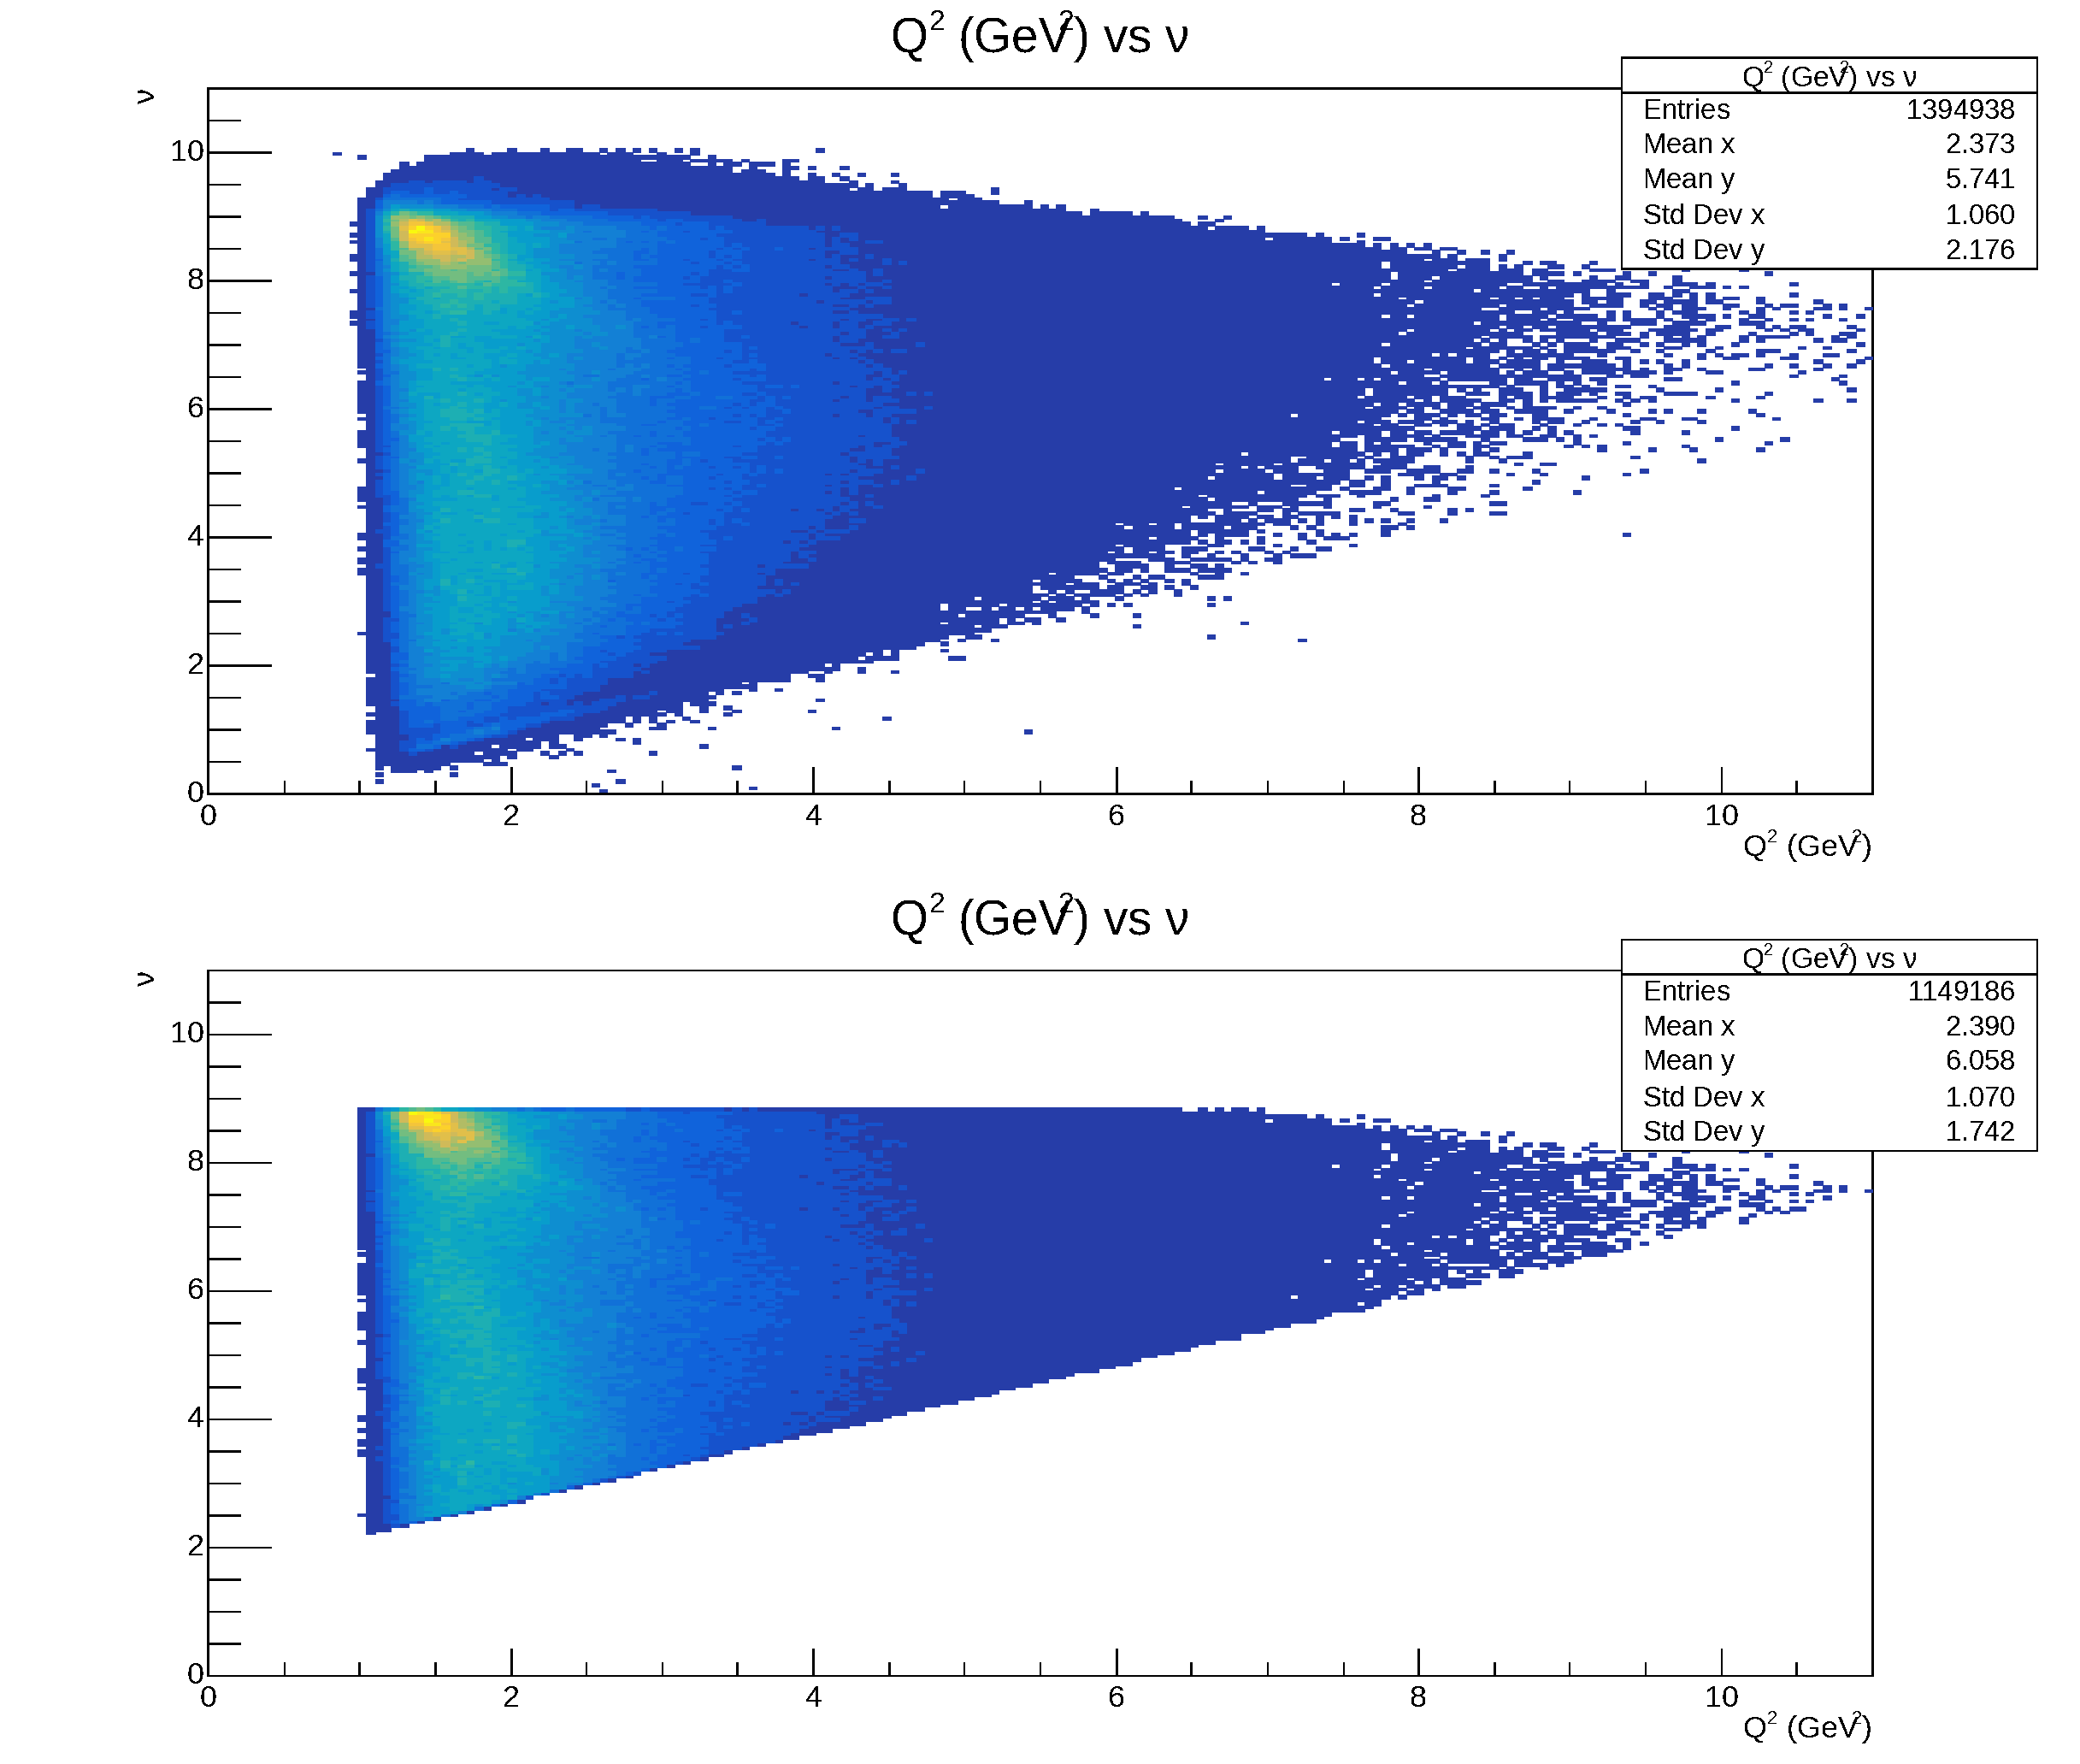
\includegraphics[width=\textwidth]{23q2_vs_nu.pdf}
        \caption[$Q^2$ vs. $\nu$ comparison]
        {$e^-$ $Q^2$ vs. $\nu$ before and after applying the $Q^2 > 1 \text{ GeV}^2$, $W^2 > 4 \text{ GeV}^2$, and $Y_b < 0.85$ cuts, run 12016.}
        \floatfoot{Source: Own elaboration, using the \href{https://github.com/bleaktwig/clas12-rge-analysis}{clas12-rge-analysis} software.}
        \label{fig::13.23::q2_vs_nu}
    \end{figure}

    Lastly, an additional cut is imposed on the Bjorken-Y ($Y_b$) of the scattered electron, given by
    \begin{equation*}
        Y_b < 0.85.
    \end{equation*}
    The Bjorken-Y ranges from 0 to 1 and is defined as
    \begin{equation*}
        Y_b = \frac{\nu}{E_b}.
    \end{equation*}
    This cut effectively mitigates the influence of extreme radiative effects, which occur when a substantial portion of the incident electron's energy is transferred to the scattered electron.

    The impact of these cuts on the $Q^2$ and $\nu$ of the scattered electron can be observed in plot \ref{fig::13.23::q2_vs_nu}.


    % !TEX root = ../main.tex
    \begin{figure}[b!]
        \centering\frame{
        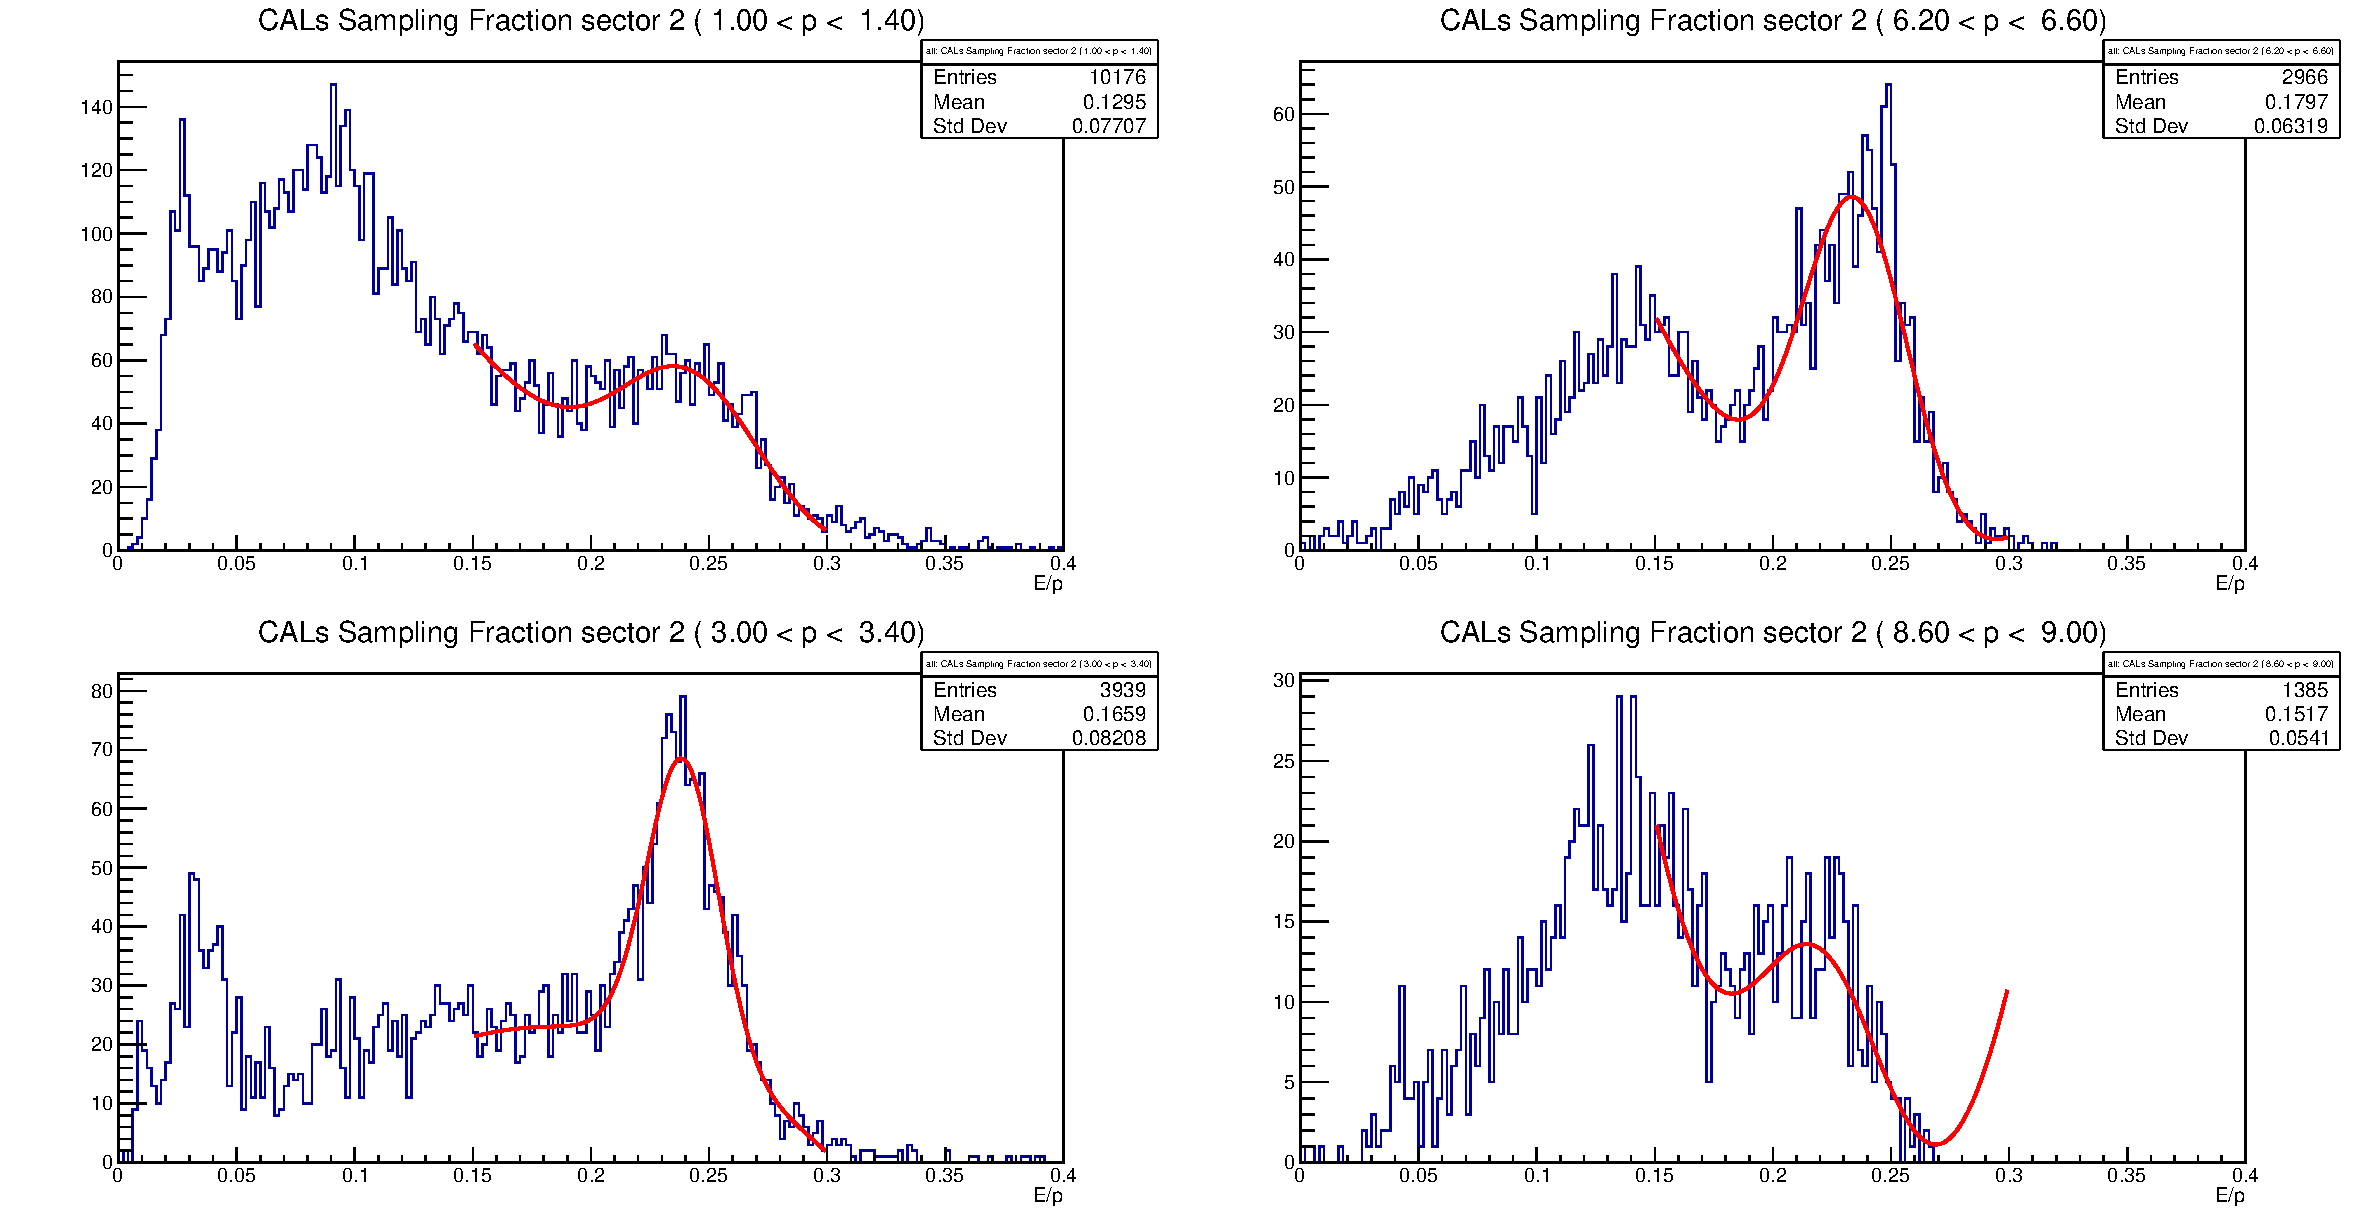
\includegraphics[width=\textwidth]{30sf_1d_plots.pdf}}
        \caption[Calorimeters $E/p$ plots]{Four $E/p$ plots describing the sum of the deposited energy per particle on all calorimeters (PCAL, ECIN, and ECOU).
        The particles' momentum is obtained from tracking and the event builder.
        As can be seen in the northwest and the southeast plots, the corner bins -- $1.00$ to $1.40$ and $8.60$ to $9.00$ GeV respectively -- are not very reliable.
        Source: Own elaboration, using the \hyperlink{github.com/bleaktwig/clas12-rge-analysis}{clas12-rge-analysis} software.}
        \label{fig::sf_1d}
    \end{figure}

\subsection{Sampling Fraction}
\label{ssec::sampling_fraction}
    The energy deposited by electrons in the active area of the calorimeters is a fraction of their total energy, $E_\text{tot}$.
    This value is proportional to their momentum, $P$, for energies above a few hundred MeV.
    Heavier particles, due to their reduced penetration capabilities, tend to lose an amount of energy independent of their momentum.
    The electron sampling fraction measures the amount of energy lost depending on the momentum of a particle.
    This allows for both the measurement of the electron's energy and the differentiation of electrons from other particles \cite{wigmans2000}.

    To obtain the sampling fraction, the hits of each calorimeter by itself (PCAL, ECIN, and ECOU) are separated into arrays, with an additional array containing the union of the other three.
    Then, these arrays of hits are separated into 20 momentum bins.
    Each bin has a size of 0.4 GeV, starting at 1.0 GeV and ending at 9.0 GeV.

    1-dimensional histograms are then created from the data in these arrays, measuring the deposited energy divided by the vertex momentum ($E/p$).
    A Gaussian fit plus a quadratic background is then applied, following the function described as

    \begin{equation*}
        f(x) = p_0 g(x, \mu, \sigma) + p_1 x^2 + p_2 x + p_3, \hspace{12pt}
        \text{where} \hspace{4pt}
        g(x, \mu, \sigma) = \frac{1}{\sigma \sqrt{2\pi}} \exp \left(-\frac{1}{2} \frac{(x - \mu)^2}{\sigma^2}\right),
    \end{equation*}

    where $\mu$ and $\sigma$ represent the mean and standard deviation of the distribution, respectively. The fit is limited to the range between $0.15$ and $0.30$ for the expected $E/p$ values for electrons based on theory.

    Examples of these plots are shown in Figure \ref{fig::sf_1d}.
    From the figure, it can be observed that there are not enough electrons in the extreme momentum ranges, such as from $1$ to $1.4$ GeV or from $8.6$ to $9$ GeV.
    Consequently, the sampling fraction fit, described in equation \eqref{eq::sampfracfit}, only considers data within the range of $1.4$ to $8.6$ GeV.

    The mean of each of these fits is then extracted to serve as data points for a sampling fraction fit.
    A polynomial fit is employed since it effectively captures the shape of these points and aligns with the reconstruction software.
    The fit is described as

    \begin{equation} \label{eq::sampfracfit}
        f(x) = p_0 \cdot \left(p_1 + \frac{p_2}{x} + \frac{p_3}{x^2}\right).
    \end{equation}

    The $E/p$ distribution vs $p$ is depicted in Figure \ref{fig::sf_2d}, together with this fit.

    \begin{figure}[t!]
        \centering\frame{
        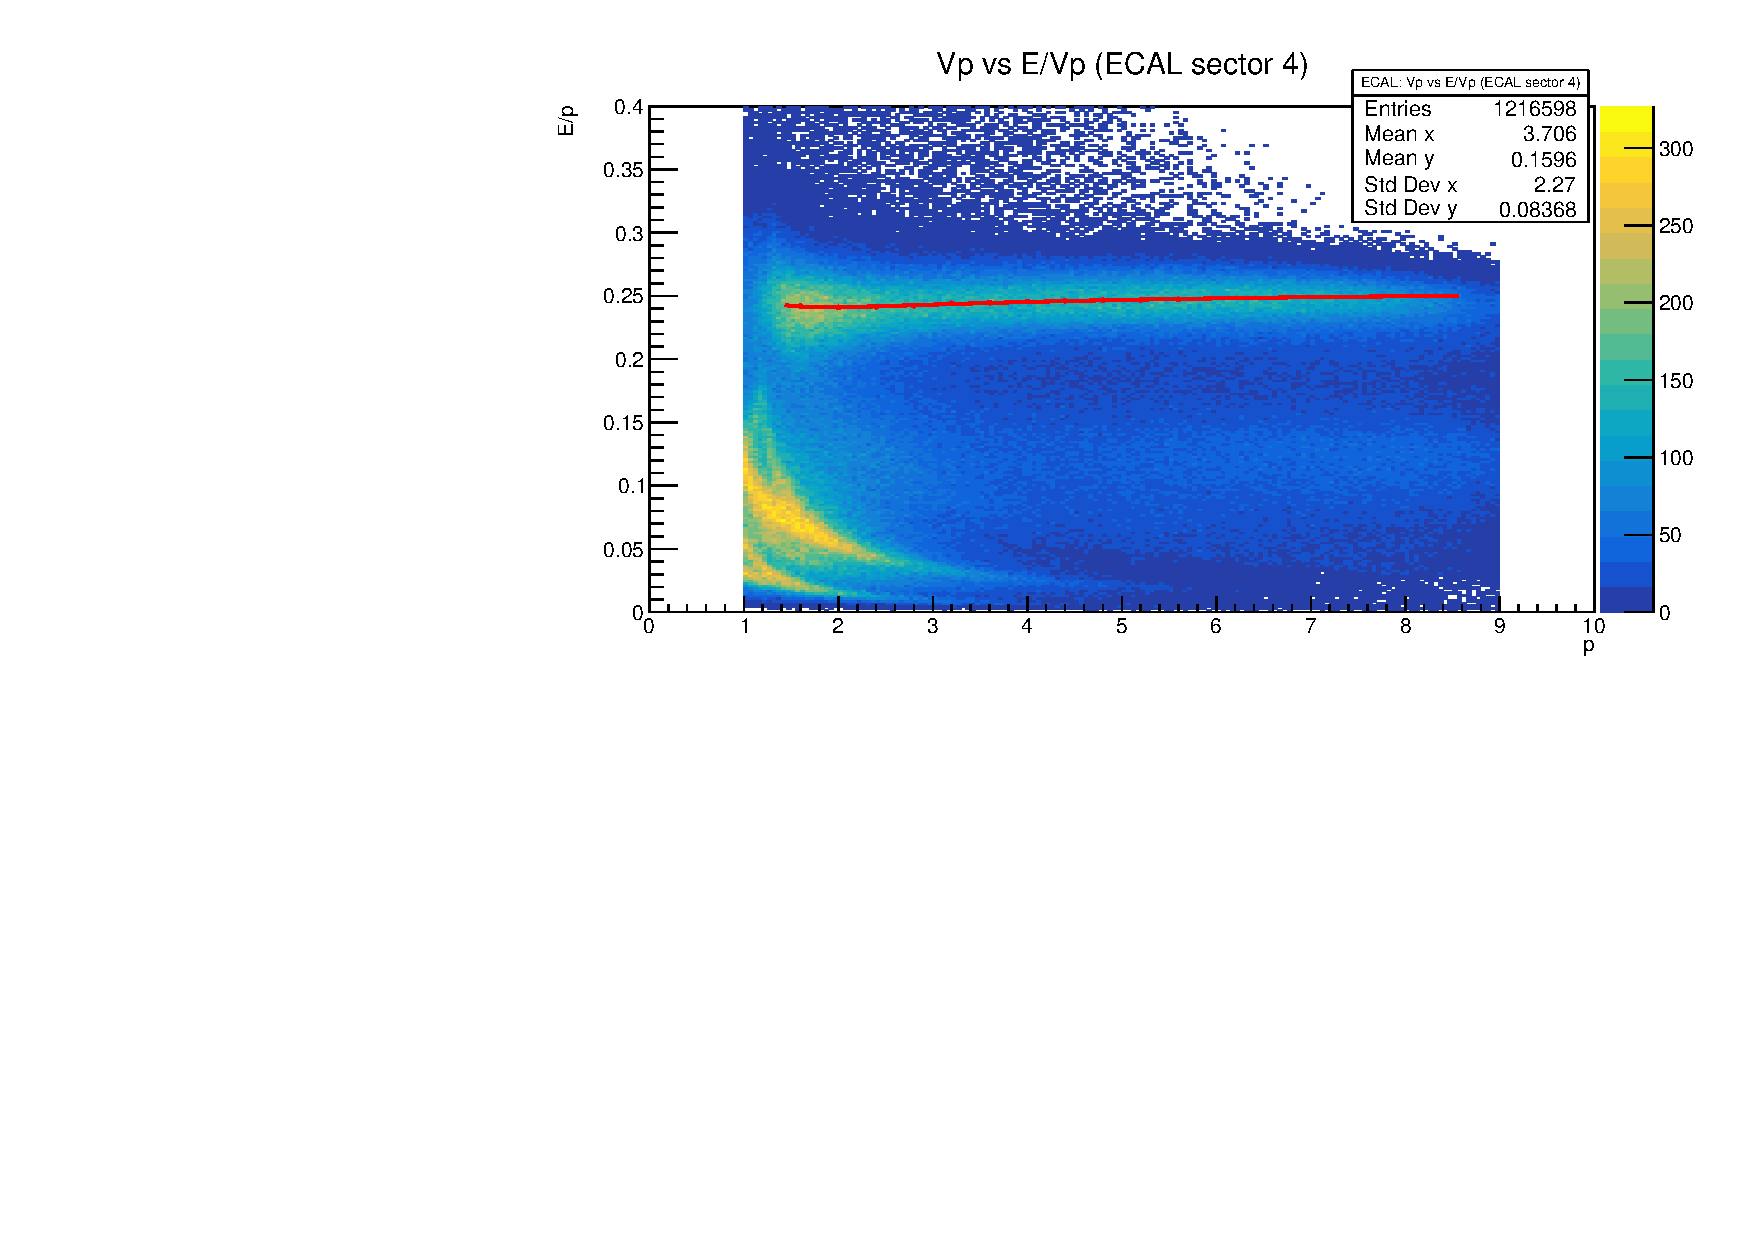
\includegraphics[width=\textwidth]{13data_analysis/img/30sf_2d_plot.pdf}}
        \caption[Calorimeters $p vs E/p$ plots]{A 2d plot showing momentum $p$ vs deposited energy divided by momentum $E/p$.
        The particle's deposited energy on all calorimeters is measured.
        Its momentum is obtained from tracking and the event builder.
        The fit follows the deposited energy of electrons to find their sampling fraction.
        Source: Own elaboration, using the \hyperlink{github.com/bleaktwig/clas12-rge-analysis}{clas12-rge-analysis} software.}
        \label{fig::sf_2d}
    \end{figure}

    Finally, the parameters of the fit are saved in plain text files, following the convention used in the CCDB.
    These parameters can be utilized later for particle identification purposes, specifically for electrons and photons.
    Furthermore, they are employed to determine the energy of electrons and photons since, as mentioned previously, not all of their energy is deposited in the calorimeters.

    % !TEX root = ../main.tex
\subsection{Acceptance Correction}
\label{ssec::acceptance_correction}
% --+ What is acceptance +------------------------------------------------------
    When discussing radiation detection, it is customary to distinguish between two types of efficiency: absolute efficiency and intrinsic detection efficiency.
    The former is defined as the fraction of events emitted by the source that are actually detected by the detector, expressed as
    \begin{equation*}
        \xi_\text{tot} = \frac{\text{events registered}}{\text{events emitted by source}}.
    \end{equation*}

    This efficiency is influenced by the detector's geometry and the probability of an interaction occurring within the detector.
    The total efficiency is also referred to as the detector acceptance.

    The total efficiency can be further decomposed into two components: the intrinsic efficiency, $\xi_{\text{int}}$, and the geometric efficiency, $\xi_{\text{geom}}$.
    The total efficiency is then given by
    \begin{equation*}
        \xi_\text{tot} = \xi_\text{int} \cdot \xi_\text{geom}.
    \end{equation*}

    The intrinsic efficiency represents the fraction of events that actually reach and are detected by the detector
    \begin{equation*}
        \xi_\text{int} = \frac{\text{events registered}}{\text{events impinging on detector}}.
    \end{equation*}

    This probability is dependent on the interaction cross-sections of the incident radiation with the detector medium.
    The intrinsic efficiency thus varies with the type of radiation, its energy, and the detector material \cite{leo1987}.

% --+ Acceptance correction through generation + simulation +-------------------
    Acceptance correction involves compensating for the total efficiency of the detector.
    To estimate this detector efficiency, a comparison is made between the total number of generated events, denoted as $N_\text{thrown}$, and the number of accepted events in a simulation of the detector, denoted as $N_\text{simul}$.
    This allows us to calculate an estimation of the detector efficiency, represented by $\tilde\xi_\text{tot}$, using
    \begin{equation*}
        \tilde\xi_\text{tot} = \frac{N_\text{simul}}{N_\text{thrown}}.
    \end{equation*}

    Naturally, the value of $\tilde\xi_\text{tot}$ is influenced by the accuracy and reliability of the event generator and simulation programs employed in the study.

% --+ Chosen bins +-------------------------------------------------------------
    The acceptance of the detector exhibits variations across the phase space of the kinematic variables.
    Therefore, in order to achieve accurate acceptance correction, the ratio $\tilde\xi_\text{tot}$ needs to be divided into bins in a five-dimensional space.
    These bins correspond to the five variables under investigation: $Q^2$, $\nu$, $z_h$, $p_T^2$, and $\phi_{PQ}$.
    To simplify the analysis process and facilitate interpretation of the results, it is advantageous to have bins of the same size for each variable.

    % TODO. I may need to update this list if I change these ranges in the future.
    \begin{itemize}
        \item
            $Q^2 = 4E_bE'\sin^2(\theta_C/2)$ is the 4-momentum transferred by the lepton probe in the lab frame, where $E_b$ is the beam energy, $E'$ is the scattered electron's energy, and $\theta_C$ is the polar angle of the scattered electron.
            The chosen bin edges are $1$, $2$, $3$, $4$, $5$, $6$, $7$, $8$, $9$, $10$, $11$ $\text{GeV}^2$.
        \item
            $\nu = E_v - E'$ is the energy transferred by the lepton probe in the lab frame.
            The chosen bin edges are $2$, $3$, $4$, $5$, $6$, $7$, $8$, $9$, and $10$ $\text{GeV}$.
        \item
            $z_h = E_h/\nu$ is the virtual photon energy fraction carried by the measured hadron, with $E_h$ being this hadron's energy.
            The chosen bin edges are $0$, $0.1$, $0.2$, $0.3$, $0.4$, $0.5$, $0.6$, $0.7$, $0.8$, $0.9$, and $1$.
        \item
            $p_T^2$ is the hadron's transverse momentum measured with respect to the virtual photon direction.
            The chosen bin edges are $0$, $0.2$, $0.4$, $0.6$, $0.8$, $1$, $1.2$, $1.4$, $1.6$, $1.8$, and $2$ $\text{GeV}^2$.
        \item
            $\phi_{PQ}$ is the angle between the leptonic plane -- the plane where the paths of the initial and scattered electrons lie -- and the hadronic plane, which contains the virtual photon and the measured hadron.
            The chosen bin edges are $-180$, $-140$, $-100$, $-60$, $-20$, $20$, $60$, $100$, $140$, and $180$ degrees.
    \end{itemize}

    To calculate the acceptance, 10 million events were initially generated in deep inelastic kinematics using LEPTO, a Monte Carlo generator specifically designed for deep inelastic lepton-nucleon scattering \cite{ingelman1997}.
    Subsequently, these events were simulated under the experimental conditions of the RG-F experiment in CLAS12 using \texttt{gemc}, which is the standard tool for CLAS12 event simulation \cite{ungaro2020gemc}.
    The simulation took into account a torus field polarity of $-1$ and a solenoid field polarity of $-0.745033$.

    Finally, the simulated events were reconstructed using \texttt{coatjava}, which is the standard tool for CLAS12 event offline reconstruction \cite{ziegler2020}.
    Further details regarding the offline reconstruction process can be found in Section \ref{sssec::offline_reconstruction}.
    The outcomes of the acceptance correction procedure are discussed in Section \ref{ssec::acceptance_correction_results}.


    \pagebreak

    % --+ Results and Conclusions +---------------------------------------------
    \graphicspath{{14results_and_conclusions/img}}
    % !TEX root = ../main.tex
\section{Results and Conclusions}
\label{14::results_and_conclusions}
    The FMT efficiency is discussed in the first section, including a brief study of it.
    Then, the second section delves into the acceptance correction results, based on the methodology described in Section \ref{13.40::acceptance_correction}.
    Following that, the study results are discussed in detail, and the conclusions of the study follow shortly thereafter.

    % !TEX root = ../main.tex
\subsection{FMT Efficiency}
\label{14.10::fmt_efficiency}
    % Low FMT efficiency + list sources.
    Compared to the alignment work described in section \ref{12::fmt_alignment_and_reconstruction}, a low FMT is observed in this analysis.
    This is evident in figure \ref{fig::14.10::vz_012933}.
    Upon inspection, three causes can be attributed to this: the application of incorrect alignment constants, a geometry effect, and a general FMT offline reconstruction issue.

    \begin{figure}[b!]
        \centering\frame{
        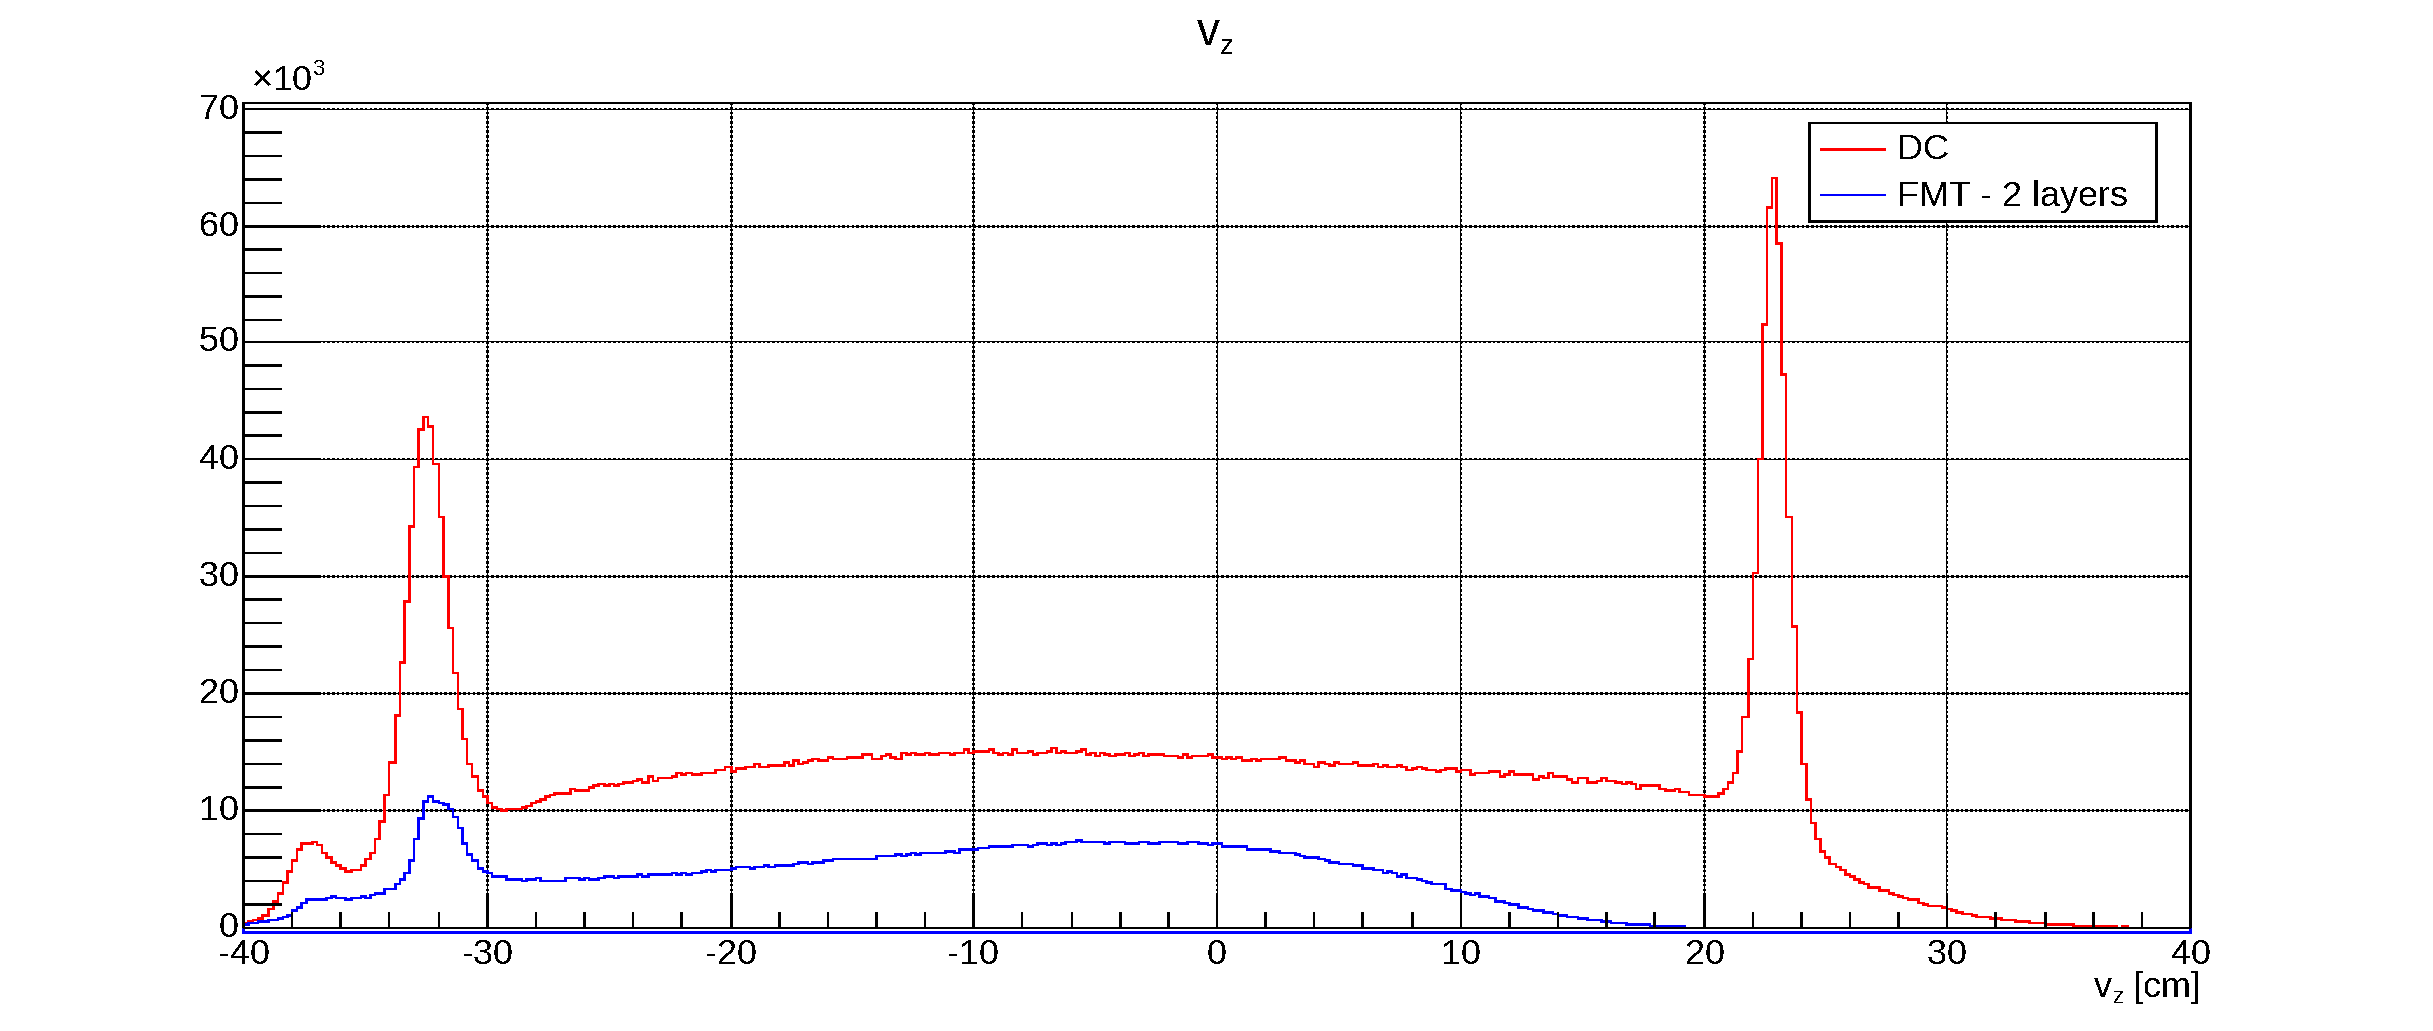
\includegraphics[width=\textwidth]{10vz_012933.pdf}}
        \caption[$v_z$ for DC and FMT, run 12933]{$v_z$ for DC (in red) and FMT (in blue). Summer 2020 data, run 12933. The wide peaks in FMT suggest an uncorrected misalignment.}
        \label{fig::14.10::vz_012933}
    \end{figure}

    % !TEX root = ../main.tex
\subsubsection{Alignment Effect}
\label{14.11::alignment_effect}
    % Introduction: The problem.
    The RG-F experiment's data is divided based on the season over which runs take place, thus there is Spring 2020 and Summer 2020 data.
    Based on the run group's guidelines, it is recommended to use Summer data, as it has seen more calibration than the Spring data.
    However, this calibration work hasn't included the FMT detector, and a strong misalignment effect is observed.

    % Cause of the problem.
    By simple visual inspection, two peaks can be clearly seen between $z = -36$ cm and $z = -30$ cm in figure \ref{fig::12.41::dc_vs_fmt_vz_11983}.
    These peaks are merged in figure \ref{fig::14.10::vz_012933}.
    As discussed in section \ref{12::fmt_alignment_and_reconstruction}, this issue comes from a lack of correction for FMT misalignments.

    % Solution.
    The simplest solution is to use Spring data.
    While more work has been put on Summer data, it mainly pertains to the central detector; unrelated to this analysis.
    Figure \ref{fig::14.11::vz_012016} shows the same $v_z$ plot from Spring 2020 run 12016.
    Both peaks are clearly visible in this plot, suggesting that misalignments are properly accounted for in the run.

    \begin{figure}[t!]
        \centering\frame{
        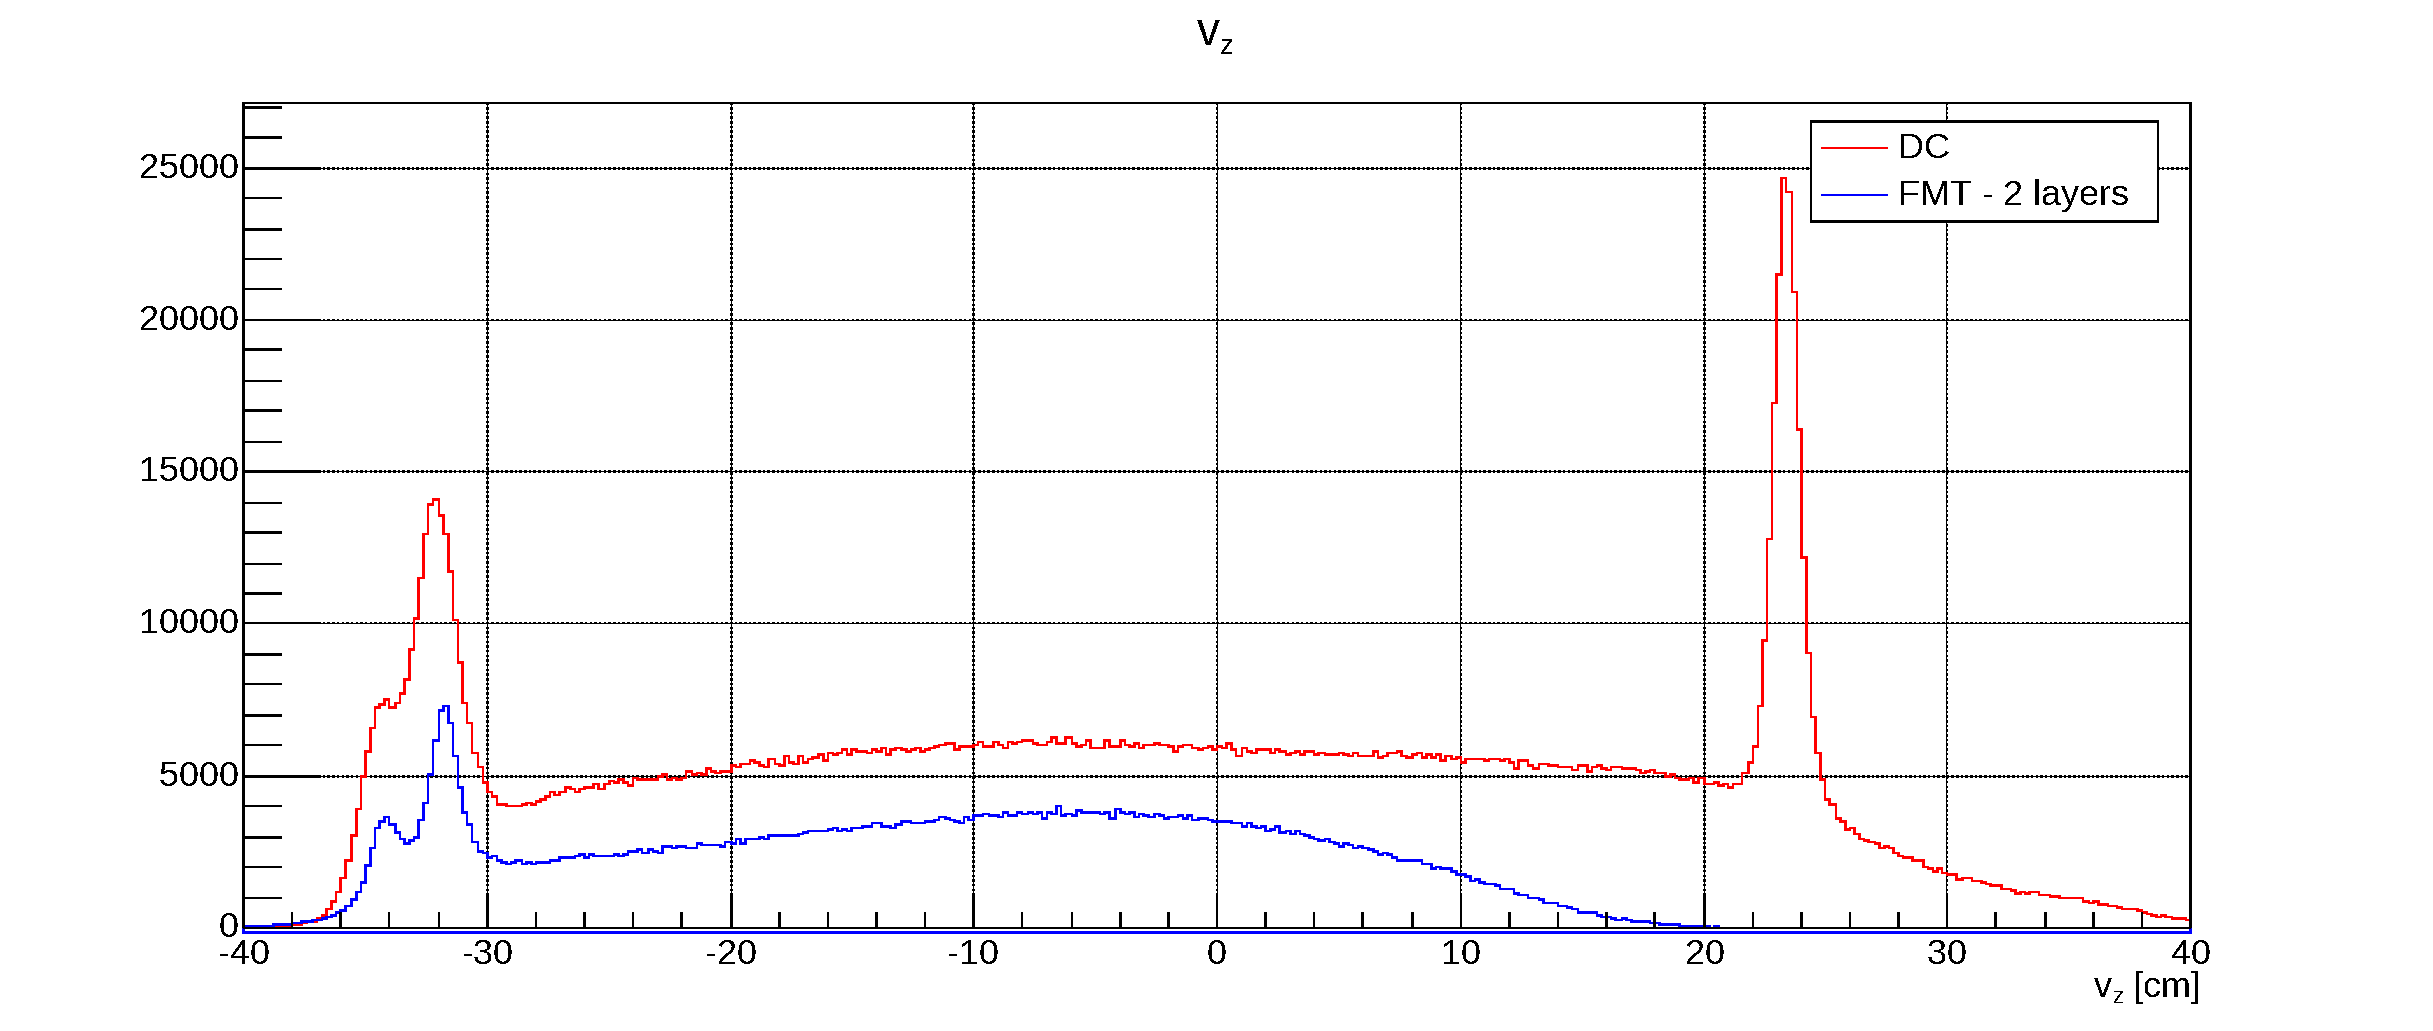
\includegraphics[width=\textwidth]{11vz_012016.pdf}}
        \caption[$v_z$ for DC and FMT, run 12016]{$v_z$ for DC (in red) and FMT (in blue). Spring 2020 data, run 12016. The upstream twin peaks can be clearly distinguished, suggesting a correct misalignment correction.}
        \label{fig::14.11::vz_012016}
    \end{figure}

    % !TEX root = ../main.tex
\subsubsection{Geometry Effect}
\label{sssec::geometry_effect}
    % The effect has already been presented and discussed before, so we're brief.
    This problem is already discussed in detail in section \ref{sssec::geometry_effect}.
    As a quick reminder, FMT sits at $z \approx 26$ cm, and it naturally performs poorly for targets to close to it.
    We can measure the strength of this effect by applying the geometry cut given by equation \eqref{eq::12.42::fmt_geometry_cut} to both DC and FMT tracks.
    Figure \ref{fig::vz_012016_geomcut} the effect of the cut when applied on figure \ref{fig::vz_012016}.
    Its effect on a $v_z$ vs $\theta$ plot can be seen on figure \ref{eq::12.42::vz_vs_theta}.

    Based on this cut and the FMT $z$ position, subsequent plots will be constrained to the range $-30 \text{[cm]} < v_z < 20 \text{[cm]}$.

    \begin{figure}[h!]
        \centering\frame{
        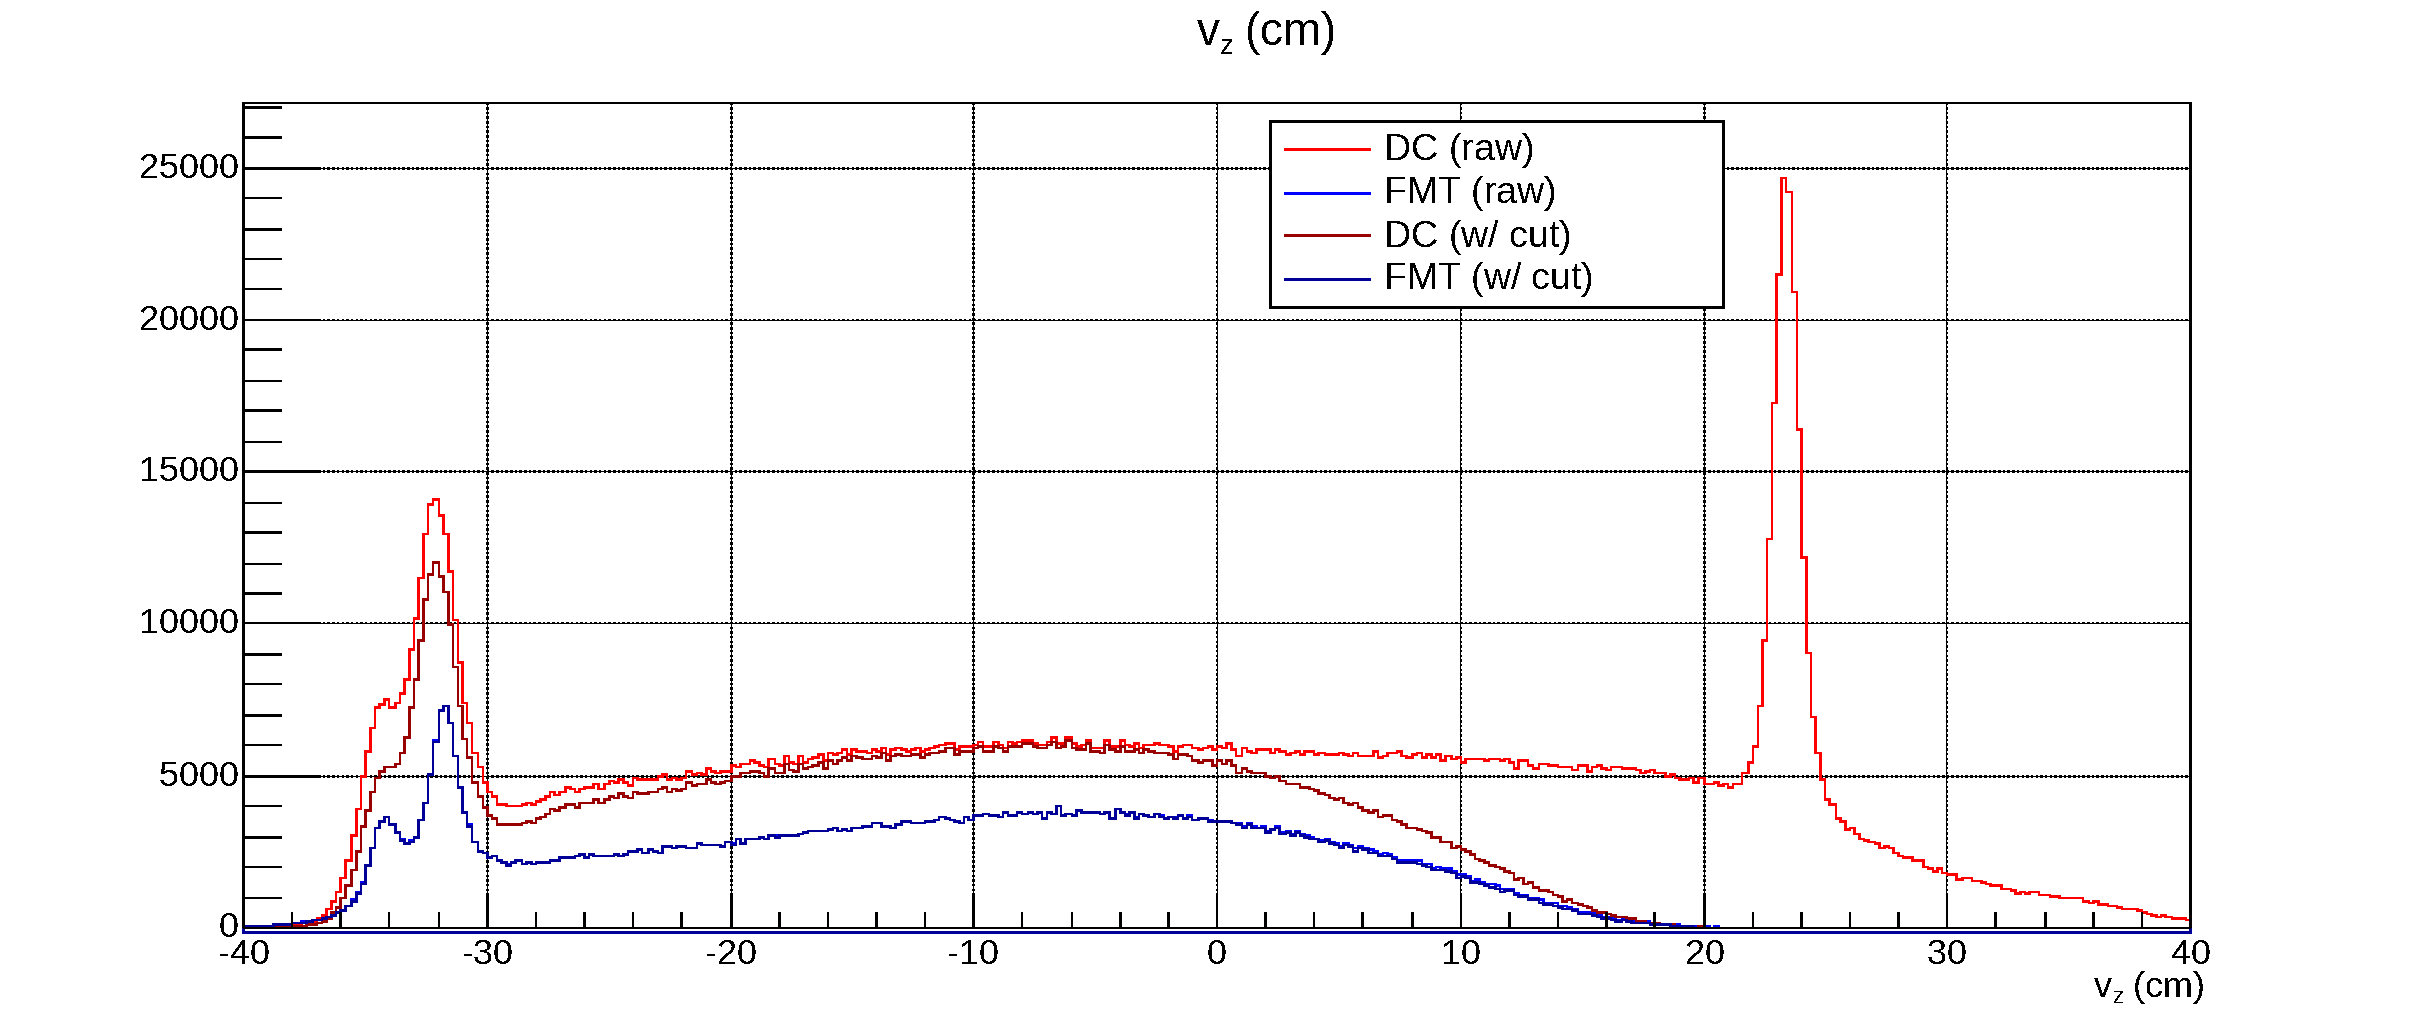
\includegraphics[width=\textwidth]{12vz_012016_geomcut.pdf}}
        \caption[$v_z$ for DC and FMT, w/ and w/out the geometry cut, run 12016]{$v_z$ for DC without the geometry cut (in red), with it (in dark red), for FMT without it (in blue), and with it (in dark blue). Spring 2020 data, run 12016. The effect is very clear on DC tracks, yet it almost doesn't affect FMT tracks.}
        \label{fig::vz_012016_geomcut}
    \end{figure}

    % !TEX root = ../main.tex
\subsubsection{Reconstruction Effect}
\label{14.13::reconstruction_effect}
    Even after correcting for both the alignment and geometry issues, FMT still has a lower efficiency when compared to that found during alignment (compare figures \ref{fig::14.12::vz_012016_geomcut} with \ref{fig::12.43::dc_vs_fmt_vz_11983_corrected}).
    After some study, the effect was found not to be correlated to run number, beam energy, or beam luminosity.
    Based on this, we can discard it being caused by hardware issues or run conditions.

    Based on this, the logical conclusion is that the effect comes from a general issue in FMT offline reconstruction.
    Finding and fixing this would be a larger project than what's contemplated in the scope of this thesis, so it's left as future work.
    For the purposes of this analysis, we'll contempt ourselves with using a large number of events, minimising statistic deficiencies.

    % !TEX root = ../main.tex
\subsubsection{Efficiency Study}
\label{14.14::efficiency_study}
% --+ Integrated. +-------------------------------------------------------------
    With all these effects accounted for, we can proceed to study the efficiency in detail.
    First, if we define FMT efficiency as the percentage of DC tracks that get accepted by FMT, we get the results in Table \ref{tab::14.14::fmt_efficiency_study} for runs 12933 (Summer 2020) and 12016 (Spring 2020), as well as the simulation described in Section \ref{13.40::acceptance_correction}.

    \begin{table}[b]
        \begin{center}
            \begin{tabularx}{0.86\textwidth}{Xlcrrcrr}
                \toprule
                & & & \multicolumn{2}{c}{\textbf{Run 12933}} & & \multicolumn{2}{c}{\textbf{Run 12016}} \\
                                    &          & & \multicolumn{1}{c}{raw} & \multicolumn{1}{c}{w/ cut} & & \multicolumn{1}{c}{raw} & \multicolumn{1}{c}{w/ cut} \\
                \midrule \midrule
                \textbf{$e^-$}      & 2 layers & & $25.1 \pm 1.5$ & $37.5 \pm 0.7$ & & $32.7 \pm 2.5$ & $53.7 \pm 0.8$ \\
                                    & 3 layers & & $ 5.6 \pm 2.7$ & $ 8.5 \pm 1.7$ & & $ 9.9 \pm 6.3$ & $16.4 \pm 3.6$ \\
                \midrule
                \textbf{$e^-\pi^+$} & 2 layers & & $ 6.5 \pm 0.2$ & $13.7 \pm 0.9$ & & $11.1 \pm 0.2$ & $28.0 \pm 1.3$ \\
                                    & 3 layers & & $ 0.3 \pm 0.1$ & $ 0.7 \pm 0.4$ & & $ 1.0 \pm 0.1$ & $ 2.7 \pm 1.4$ \\
                \midrule
                \textbf{$e^-\pi^-$} & 2 layers & & $ 5.6 \pm 0.0$ & $14.2 \pm 1.0$ & & $ 8.9 \pm 0.4$ & $29.5 \pm 1.4$ \\
                                    & 3 layers & & $ 0.3 \pm 0.0$ & $ 0.7 \pm 0.5$ & & $ 0.9 \pm 0.3$ & $ 2.9 \pm 1.6$ \\
                \bottomrule
            \end{tabularx}
        \end{center}
        \caption[FMT efficiency study results]
        {Results of the FMT efficiency study performed in $\%$.}
        \label{tab::14.14::fmt_efficiency_study}
    \end{table}

    % --+ Error estimation +----------------------------------------------------
    To estimate the efficiency of one FMT layer and the associated errors for the two types of tracks, we define $P(L_n)$ as the probability of layer $n$ detecting a particle, with $1 \leq n \leq 3$.
    Assuming that all layers have the same efficiency, denoted as $E_1$,
    \begin{equation*}
        P(L_1) = P(L_2) = P(L_3) = E_1,
    \end{equation*}
    the efficiency $E_3$ for 3-layer tracks can be obtained using the probabilities $P(L_n)$ as follows
    \begin{align}
        E_3 &= P(L_1)P(L_2)P(L_3)
        \nonumber \\
        E_3 &= E_{1(3)}^3,
        \label{eq::14.14::efficiency3}
    \end{align}
    where $E_{1(3)}$ is the 1-layer efficiency estimated from 3-layer tracks.

    For 2-layer tracks, the efficiency $E_2$ can be obtained as
    \begin{align}
        E_2 &= P(L_1)P(L_2)\left(1 - P(L_3)\right)                \nonumber \\
             &\hspace{24pt} + P(L_2)P(L_3)\left(1 - P(L_1)\right) \nonumber \\
             &\hspace{24pt} + P(L_3)P(L_1)\left(1 - P(L_2)\right) \nonumber \\
             &\hspace{24pt} + P(L_1)P(L_2)P(L_3)                  \nonumber \\
        E_2 &= 3E_{1(2)}^2\left(1 - E_{1(2)}\right) + E_{1(3)}^3
            \nonumber \\
        E_2 &= 3E_{1(2)}^2 \cdot \left( 1 - E_{1(2)} \right) + E_3,
        \label{eq::14.14::efficiency2}
    \end{align}
    where $E_{1(2)}$ is the 1-layer efficiency estimated from 2-layer tracks.

    From \eqref{eq::14.14::efficiency3}, we can estimate $E_{1(3)}$ as
    \begin{equation}
        E_{1(3)} = \sqrt[3]{E_3}.
        \label{eq::14.14::efficiency1(3)}
    \end{equation}
    In contrast, $E_{1(2)}$ cannot be obtained explicitly from \eqref{eq::14.14::efficiency2}, but it can be estimated numerically.

    Using equations \eqref{eq::14.14::efficiency2} and \eqref{eq::14.14::efficiency1(3)}, we can estimate the weighted average efficiency $\xoverline{E_1}$ as
    \begin{equation*}
        \xoverline{E_1} = \frac{4E_{1(2)} + E_{1(3)}}{5},
    \end{equation*}
    where the weights are assigned based on the number of ways 2 and 3-layer tracks can be obtained, 4 and 1, respectively.

    From $\xoverline{E_1}$, we can estimate the errors on $E_{1(2)}$ and $E_{1(3)}$ as
    \begin{align*}
        \delta(E_{1(2)}) = |\xoverline{E_1} - E_{1(2)}|, \\
        \delta(E_{1(3)}) = |\xoverline{E_1} - E_{1(3)}|.
    \end{align*}

    To propagate these errors to the efficiencies $E_2$ and $E_3$, we use the variance formula
    \begin{equation*}
        \delta\left(f(x)\right) = \frac{\partial f(x)}{\partial x} \cdot \delta(x),
    \end{equation*}
    where $\delta(E_2)$, obtained from equation \eqref{eq::14.14::efficiency2}, is
    \begin{align*}
        \delta(E_2) &= \frac{\partial}{\partial E_{1(2)}} \left( 3E_{1(2)}^2 - 3E_{1(2)}^3 + E_{1(3)}^3 \right)
            \cdot \delta \left( E_{1(2)} \right) \\
        \delta(E_2) &= \left( 6E_{1(2)} - 9E_{1(2)}^2 \right) \cdot \delta \left( E_{1(2)} \right)
    \end{align*}
    and $\delta(E_3)$, obtained from equation \eqref{eq::14.14::efficiency3}, is
    \begin{align*}
        \delta(E_3) &= \frac{\partial}{\partial E_{1(3)}} \left( E_{1(3)}^3 \right) \cdot \delta \left( E_{1(3)} \right) \\
        \delta(E_3) &= 3E_{1(3)}^2 \cdot \delta \left( E_{1(3)} \right).
    \end{align*}

    A Python script was written to calculate $E_2$ and $E_3$ from each measurement shown in Table \ref{tab::14.14::fmt_efficiency_study}.
    The script is included in Appendix \ref{20.03::fmt_layer_efficiency_error_estimation}.
    The corresponding errors were obtained this way, and are included in the table.

    % --+ Conclusions drawn from table +----------------------------------------
    The table illustrates the positive impact of switching to Spring 2020 data and applying the geometry cut.
    The switch results in a $30.1\%$ increase in detected trigger electrons, as well as a $70.8\%$ increase for positive pions and a $58.9\%$ increase for negative pions.
    Furthermore, by applying the geometry cut based on $v_z$ and $\theta$, an additional $64.2\%$ increase in trigger electrons is achieved, resulting in a total increase of $113.9\%$.
    The pion yield experiences a substantial enhancement, with positive pions increasing by $150.2\%$ and negative pions increasing by $231.5\%$, resulting in a total increase of $330.8\%$ and $426.8\%$, respectively.

% --+ Separated. +--------------------------------------------------------------
    Next, we need to ensure that we are not introducing a systematic error by applying these corrections.
    To achieve this, we must investigate the effect of the geometry cut on different detected variables for electrons ($e^-$), positive pions ($e^-\pi^+$), and negative pions ($e^-\pi^-$).
    Based on the definition of the cut, we anticipate a strong correlation between efficiency and $v_z$ and $\theta$, and at most a weak correlation with $\phi$ and $p$.

    \begin{figure}
        % vz.
        \begin{subfigure}[b]{\textwidth}
            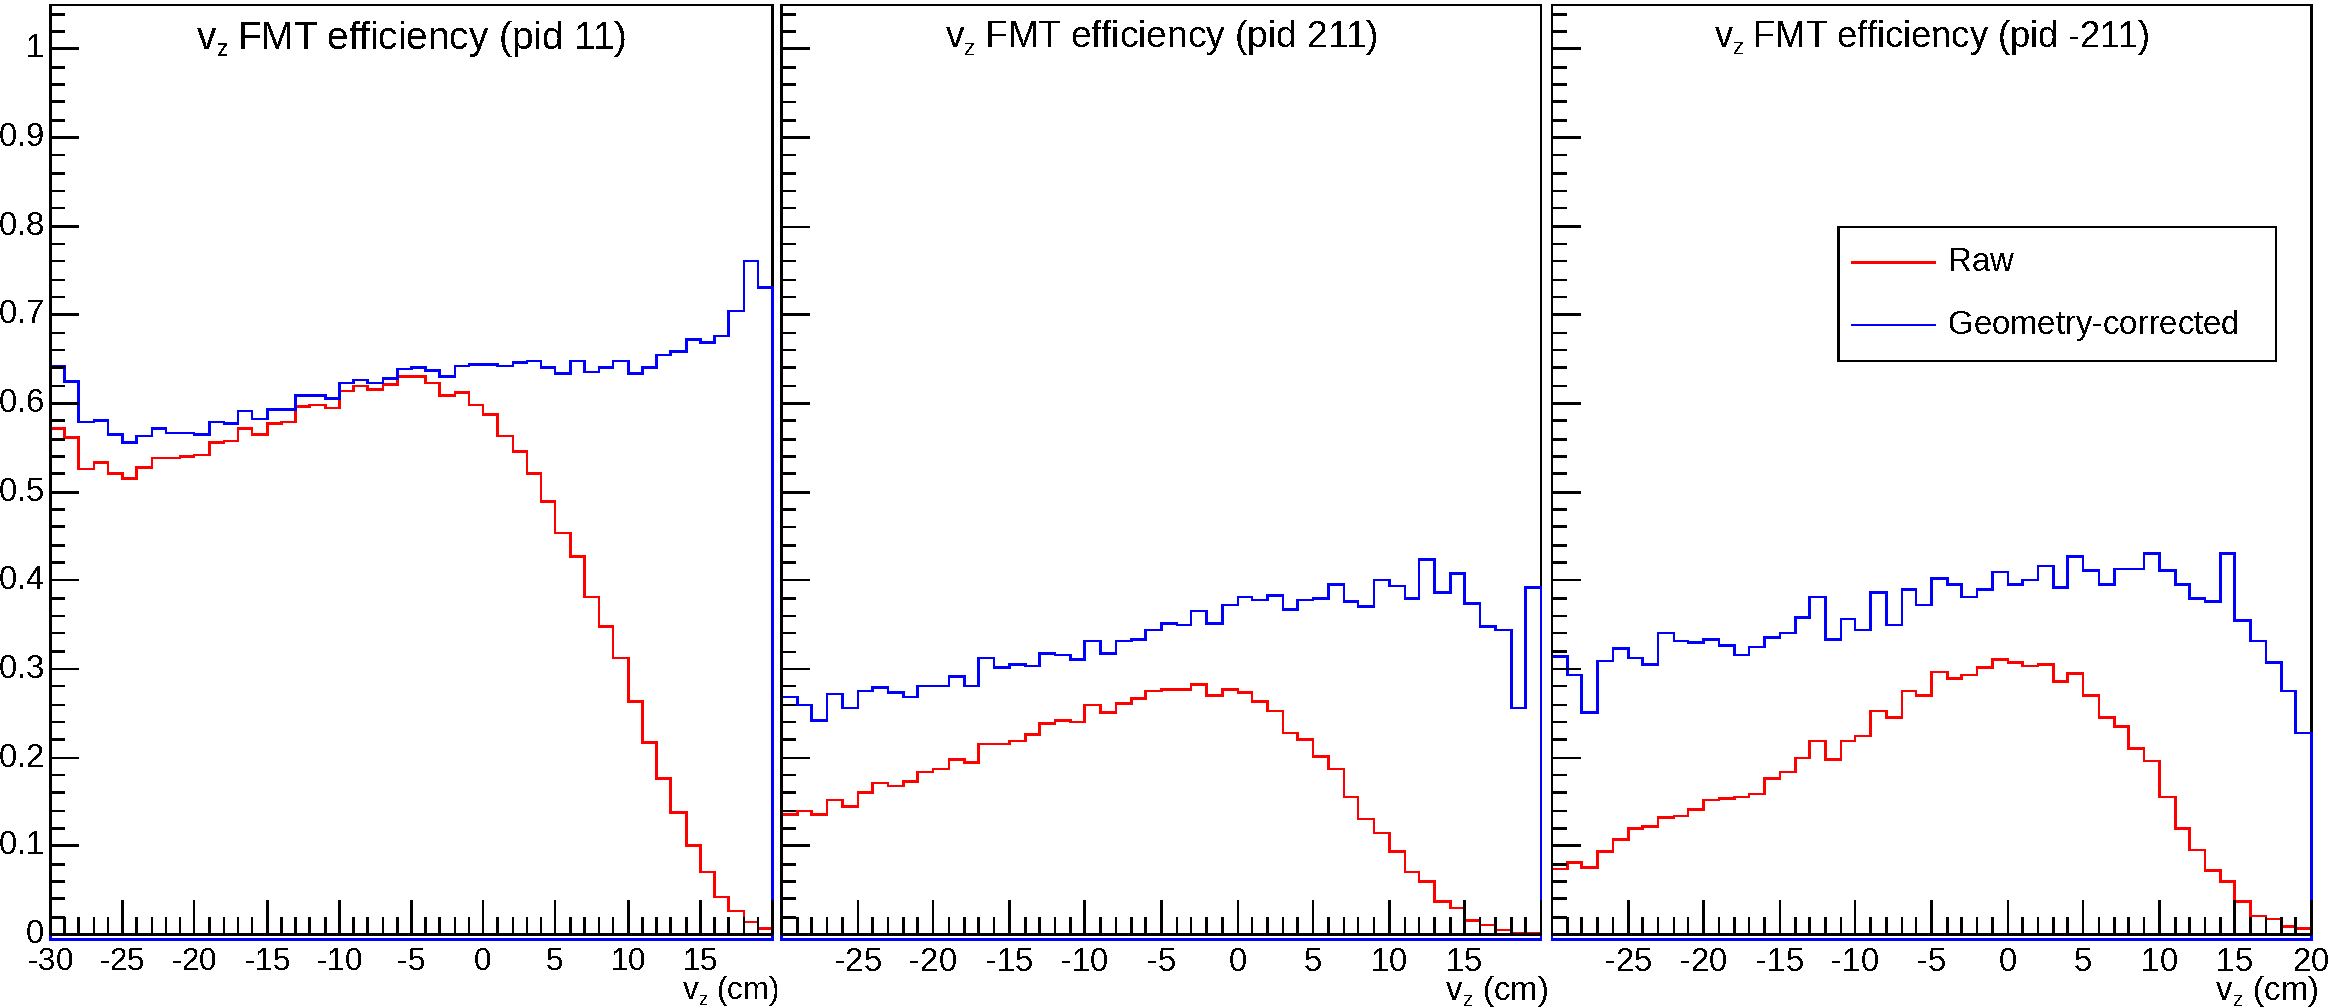
\includegraphics[width=\textwidth]{14vz_efficiency.pdf}
            \caption{$v_z$ FMT efficiency}
            \label{fig::14.14::fmt_efficiency_vz}
        \end{subfigure}
        % theta.
        \begin{subfigure}[b]{\textwidth}
            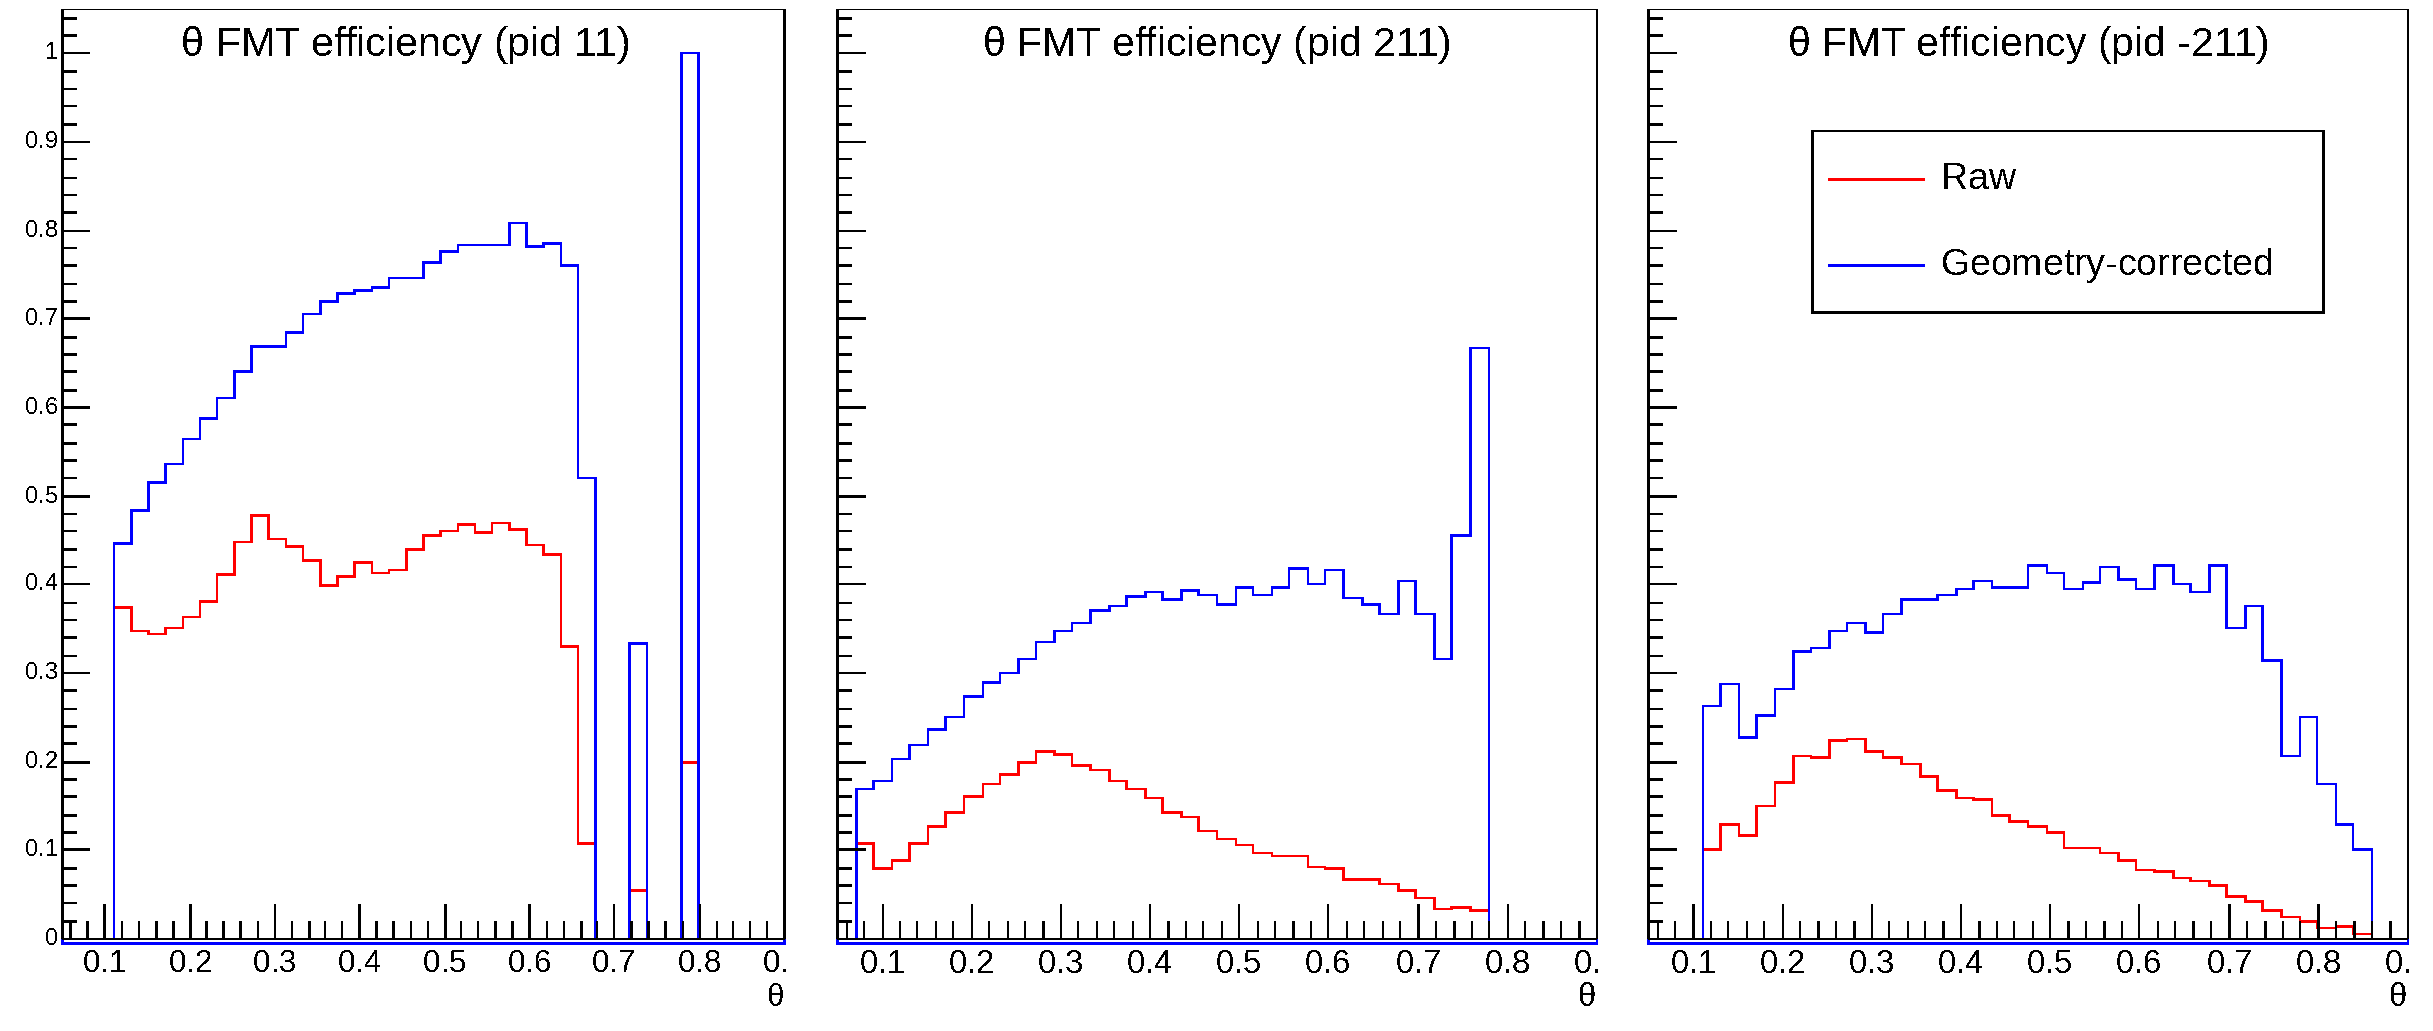
\includegraphics[width=\textwidth]{14theta_efficiency.pdf}
            \caption{$\theta$ FMT efficiency.}
            \label{fig::14.14::fmt_efficiency_theta}
        \end{subfigure}
        % p.
        \begin{subfigure}[b]{\textwidth}
            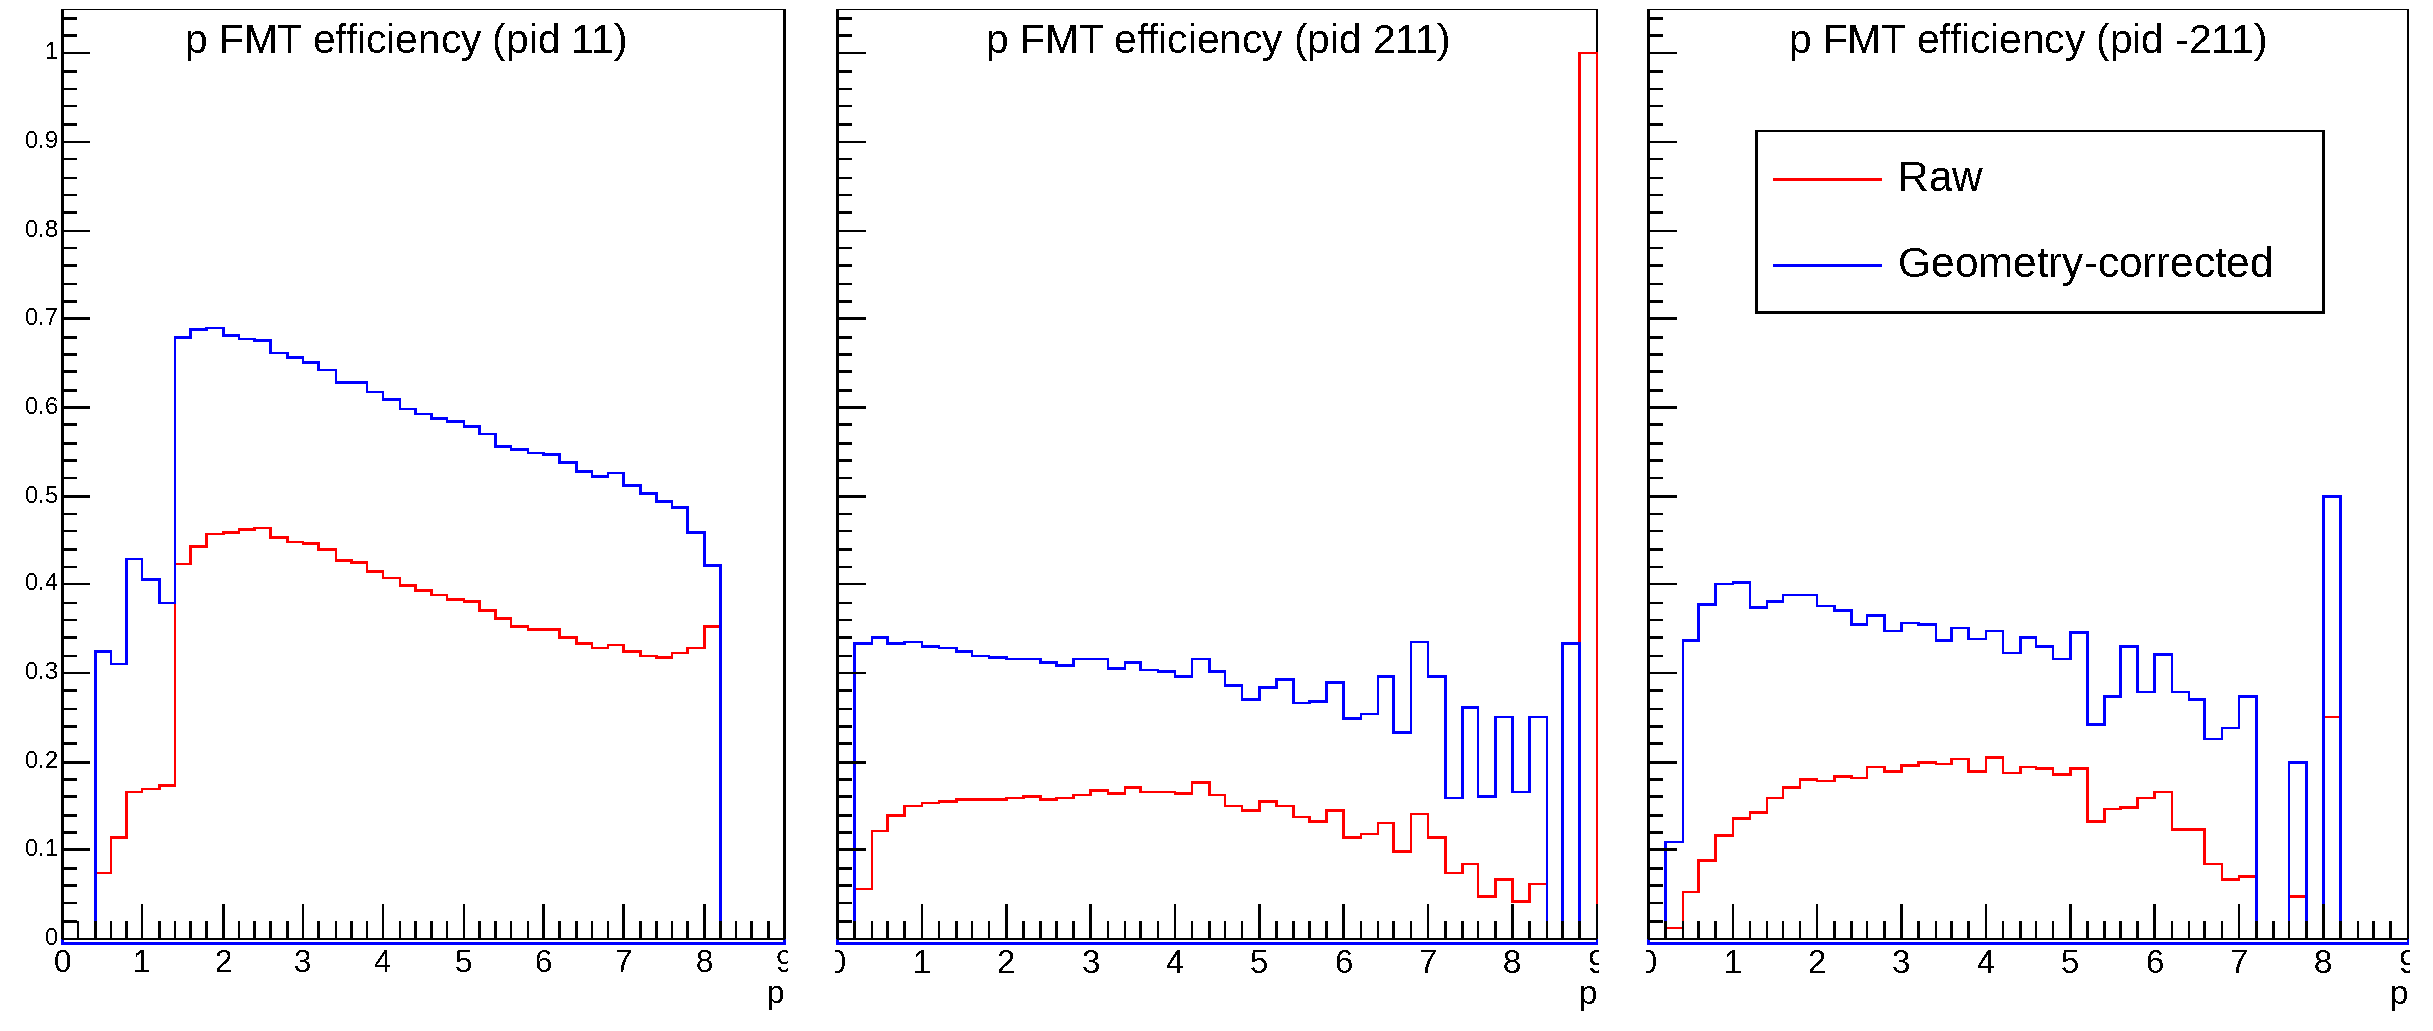
\includegraphics[width=\textwidth]{14p_efficiency.pdf}
            \caption{$p$ FMT efficiency.}
            \label{fig::14.14::fmt_efficiency_p}
        \end{subfigure}

        \caption[$v_z$, $\theta$, and $p$ FMT efficiencies for $e^-$, $e^-\pi^+$, and $e^-\pi^-$]
        {$v_z$, $\theta$, and $p$ FMT efficiencies for $e^-$, $e^-\pi^+$, and $e^-\pi^-$.
        FMT efficiency is defined as the percentage of DC tracks that are detected by 2 FMT layers.
        Run 12016.}
        \floatfoot{Source: Own elaboration, using the \href{https://github.com/bleaktwig/clas12-rge-analysis}{clas12-rge-analysis} software.}
        \label{fig::14.14::fmt_efficiencies}
    \end{figure}

    \begin{figure}
        % phi efficiency.
        \begin{subfigure}[b]{\textwidth}
            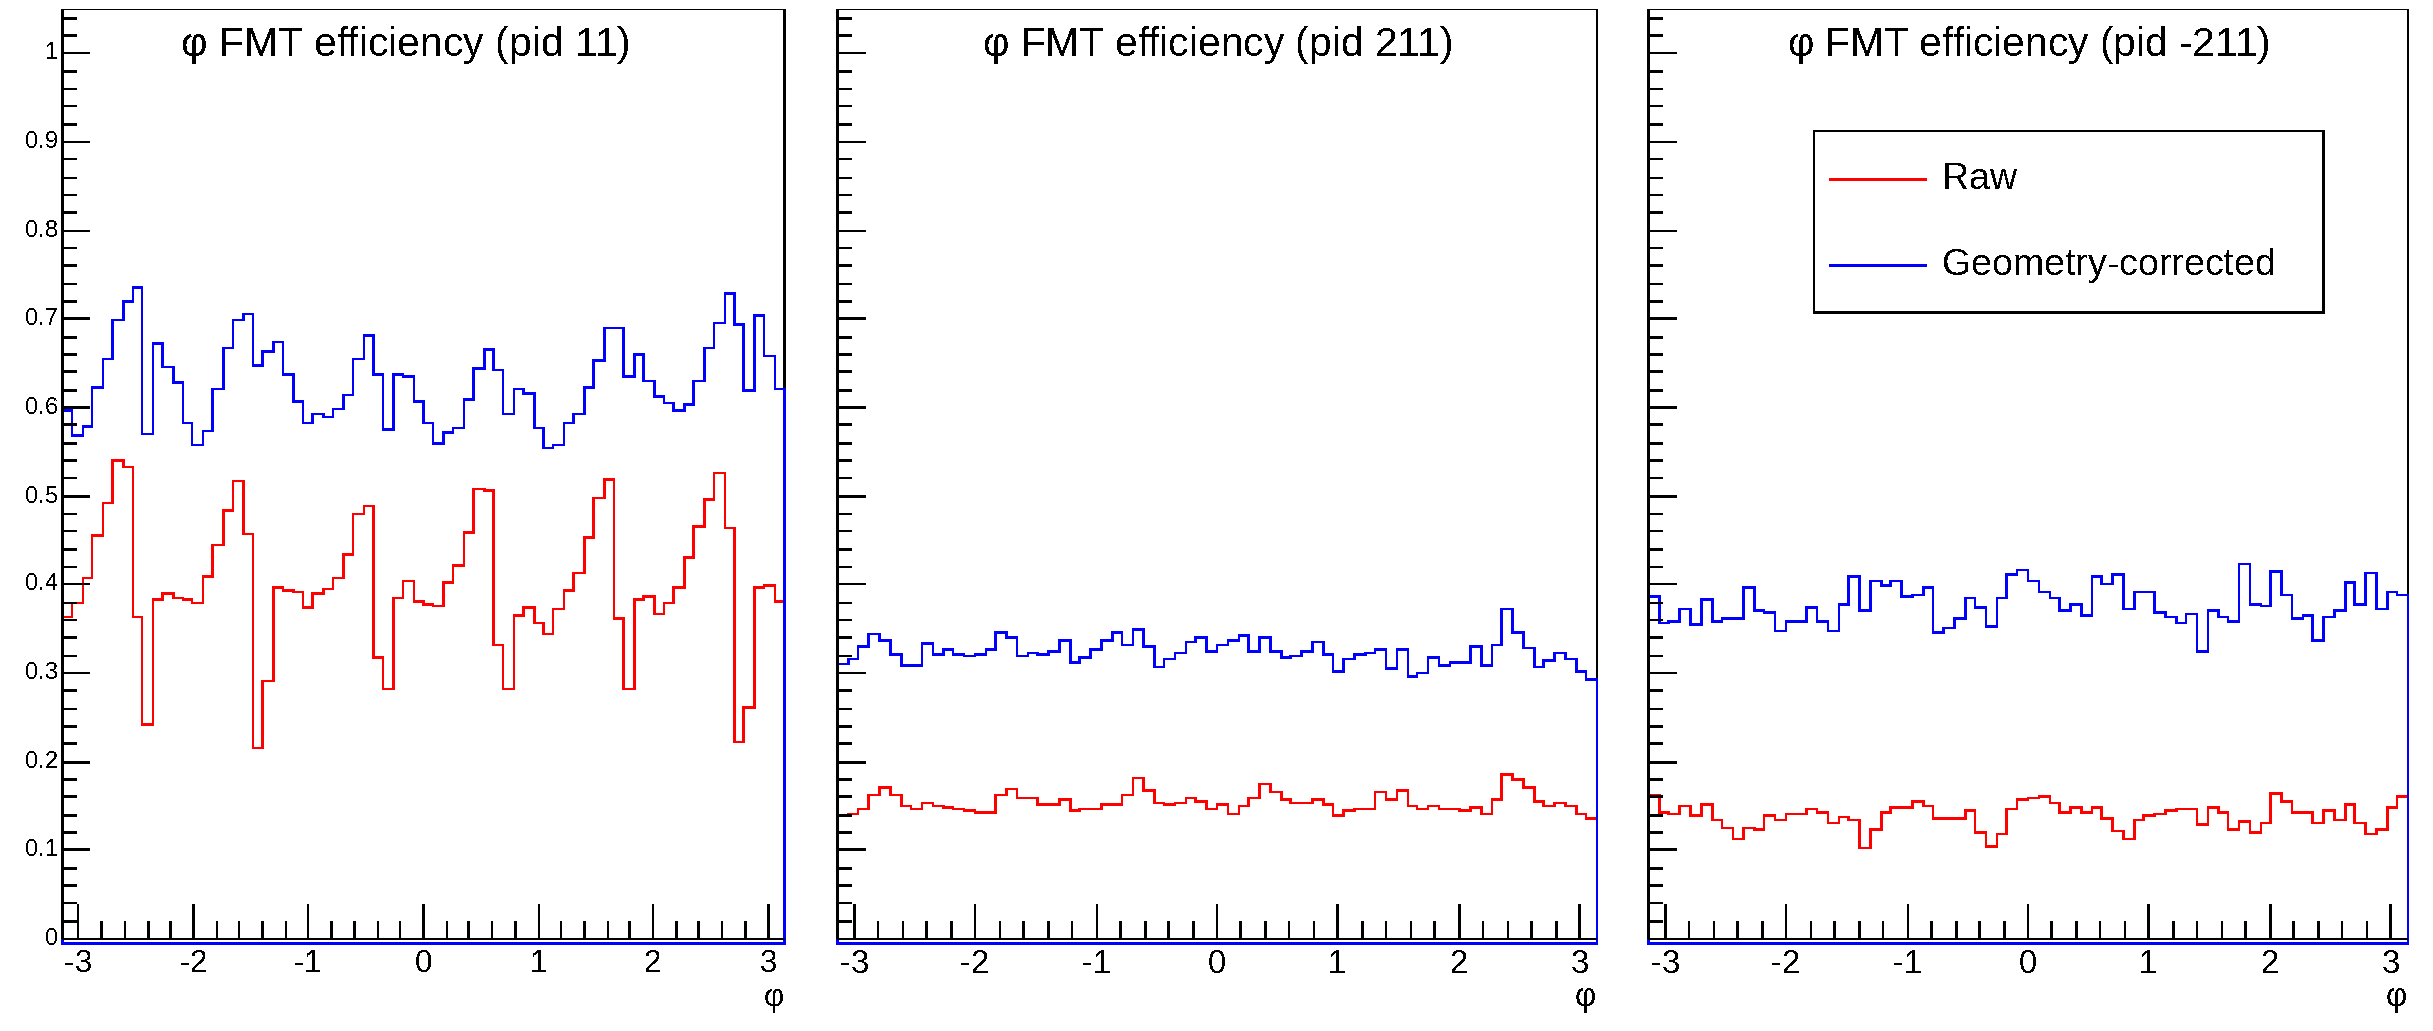
\includegraphics[width=\textwidth]{14phi_efficiency.pdf}
            \caption{$\phi$ FMT efficiency for $e^-$, $e^-\pi^+$, and $e^-\pi^-$.
            FMT efficiency is defined as the percentage of DC tracks that are detected by 2 FMT layers.}
            \label{fig::14.14::fmt_efficiency_phi}
        \end{subfigure}
        % geometry cut effect.
        \begin{subfigure}[b]{\textwidth}
            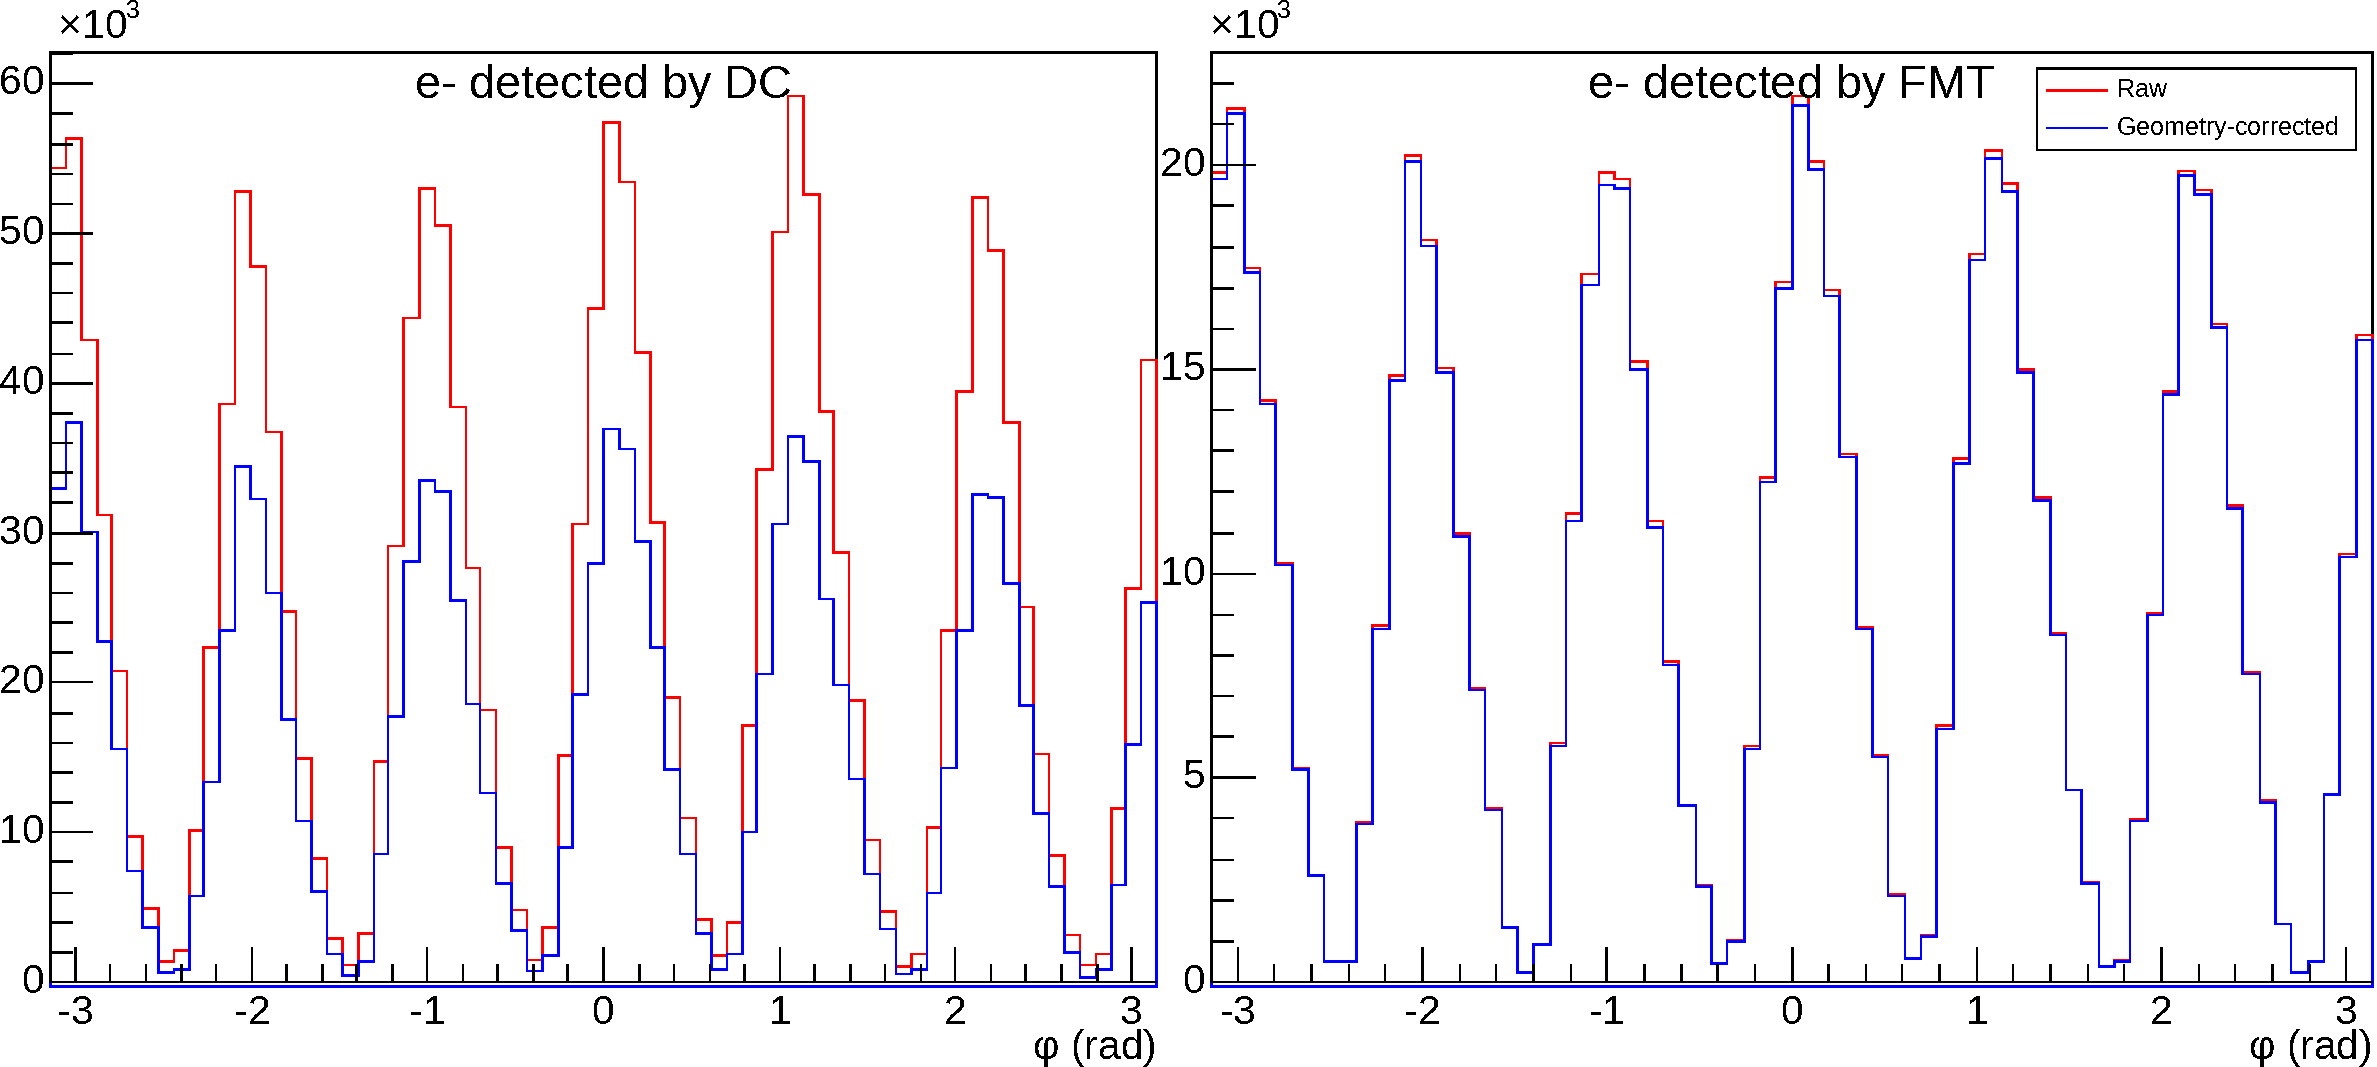
\includegraphics[width=\textwidth]{14phi_geomcut.pdf}
            \caption{Number of electrons detected in terms of $\phi$ for DC and FMT.}
            \label{fig::14.14::phi_geomcut}
        \end{subfigure}

        \caption[$\phi$ efficiency and geometry cut study]
        {$\phi$ FMT efficiency and number of $e^-$ detected for DC and FMT.
        Run 12016.}
        \floatfoot{Source: Own elaboration, using the \href{https://github.com/bleaktwig/clas12-rge-analysis}{clas12-rge-analysis} software.}
        \label{fig::14.14::phi_study}
    \end{figure}

    Our prediction is validated by Figures \ref{fig::14.14::fmt_efficiency_vz} and \ref{fig::14.14::fmt_efficiency_theta}.
    The efficiency displays a pronounced dependence on both $v_z$ and $\theta$ for all three particles under study.
    It is worth noting that the dependence is more pronounced for electrons compared to pions.
    This outcome aligns with expectations, as the only accepted pions are those detected in events where an electron is also detected.
    Thus, the ``final'' pion efficiency incorporates the combined detector efficiencies for electrons and pions.

    Next, Figure \ref{fig::14.14::fmt_efficiency_p} confirms our expectation that there is no strong correlation between efficiency and momentum.

    Last, we examine the $\phi$ efficiency, as depicted in Figure \ref{fig::14.14::fmt_efficiency_phi}.
    Our prediction holds true for both positive and negative pions, as the efficiency demonstrates no dependence on the value of $\phi$.
    However, in the case of electrons, upon initial inspection, the sharp valleys appear less prominent after applying the geometry cut.

    Nevertheless, this is merely a visual effect.
    When we tally the number of electrons detected by the DC and FMT, the valleys become more pronounced in the DC, while they remain the same in the FMT.
    Consequently, the increase in FMT efficiency becomes more pronounced in these valleys, as demonstrated in Figure \ref{fig::14.14::phi_geomcut}.

    As can be seen in Table \ref{tab::14.14::fmt_efficiency_study} and Figures \ref{fig::14.14::fmt_efficiencies} and \ref{fig::14.14::phi_study}, the pion efficiency for 3-layer tracks does not exceed $3\%$.
    Consequently, it is not practical to work exclusively with FMT tracks that traverse all three FMT layers in this study.
    For the remainder of the document, 2 and 3-layer tracks will be considered together, and will be collectively referred to as FMT tracks.


    % !TEX root = ../main.tex
\subsection{Acceptance Correction Results}
\label{14.20::acceptance_correction_results}
    % !TEX root = ../main.tex
\subsubsection{Electron Variables}
\label{14.21::electron_variables}
    The acceptance of the scattered electron variables $Q^2$ and $\nu$ is presented in Figure \ref{fig::14.21::electron_acc}.
    Each one is shown in an integrated kinematical region for the other variable.

    \begin{figure}[t!]
        \centering
        % Q2.
        \begin{subfigure}[b]{\textwidth}
            \centering
            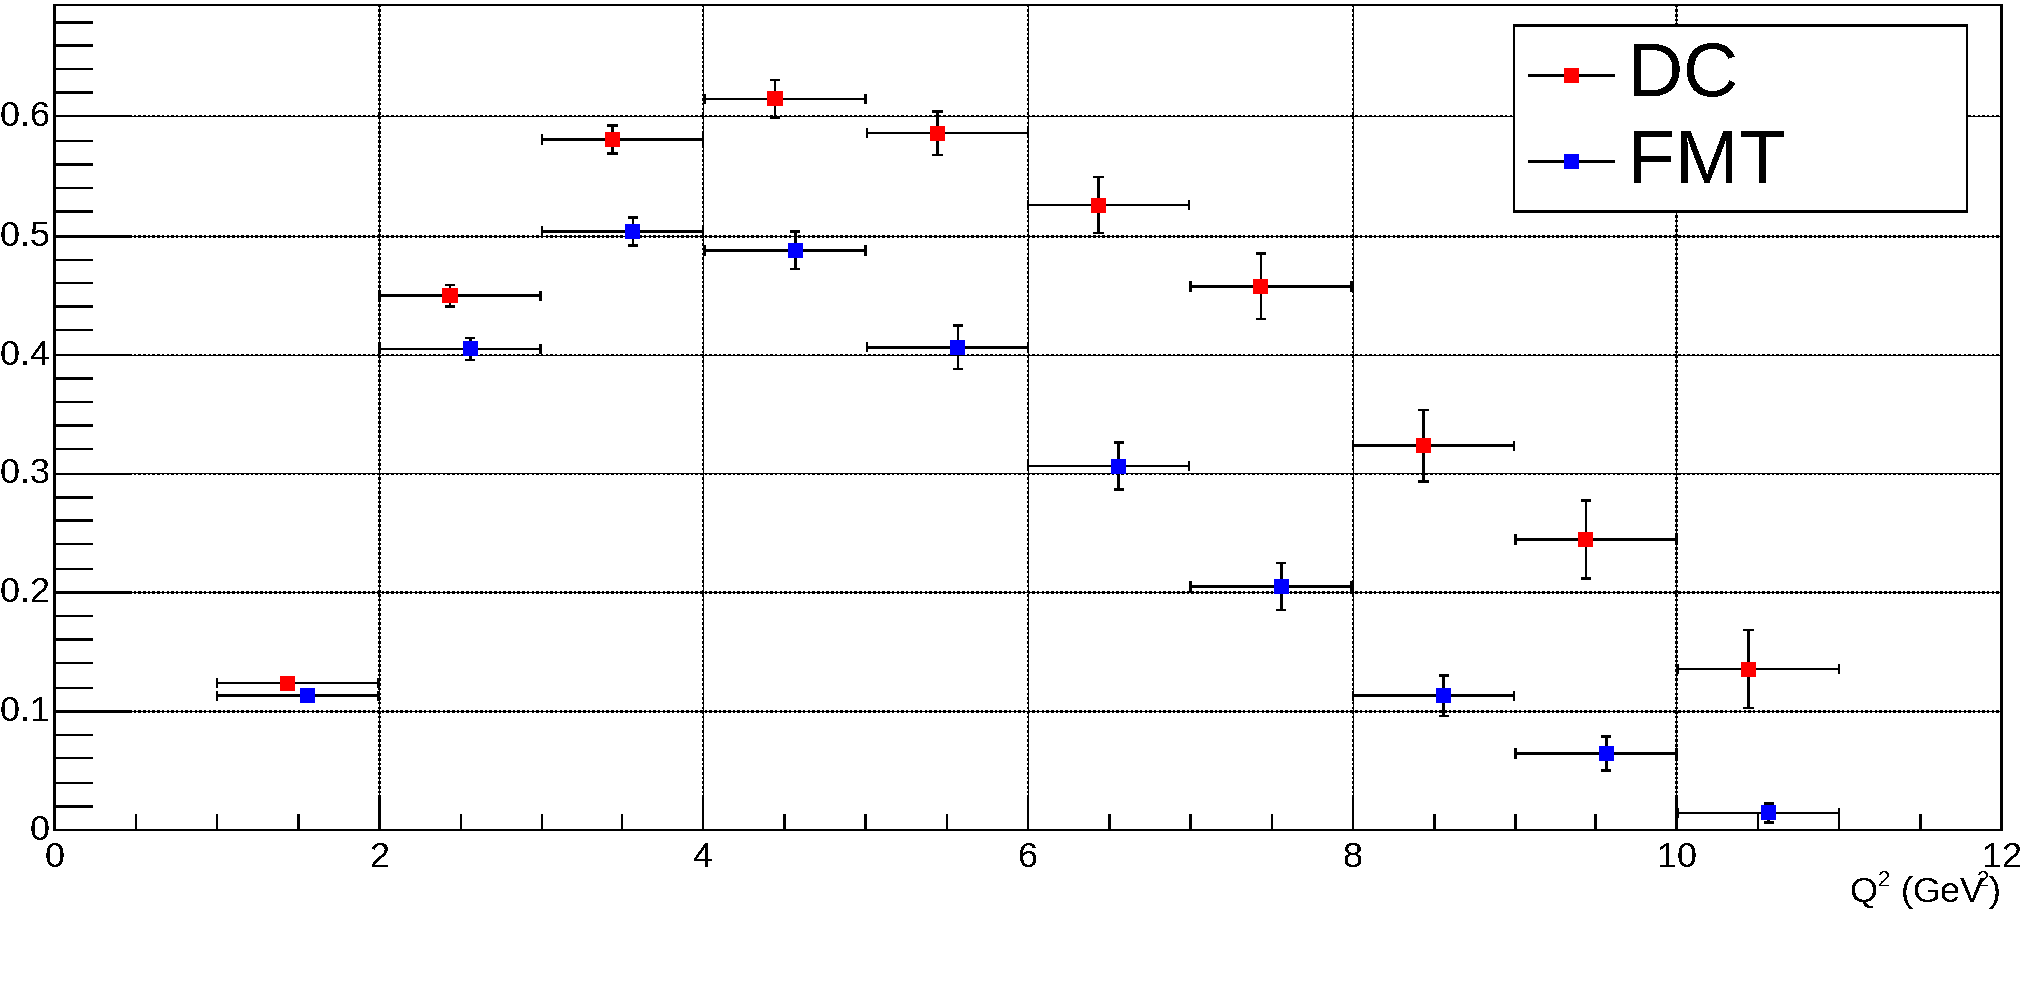
\includegraphics[width=\textwidth]{21q2_acc.pdf}
            \caption{$Q^2$ acceptance.}
            \label{fig::14.21::q2_acc}
        \end{subfigure}
        \hfill
        % nu.
        \begin{subfigure}[b]{\textwidth}
            \centering
            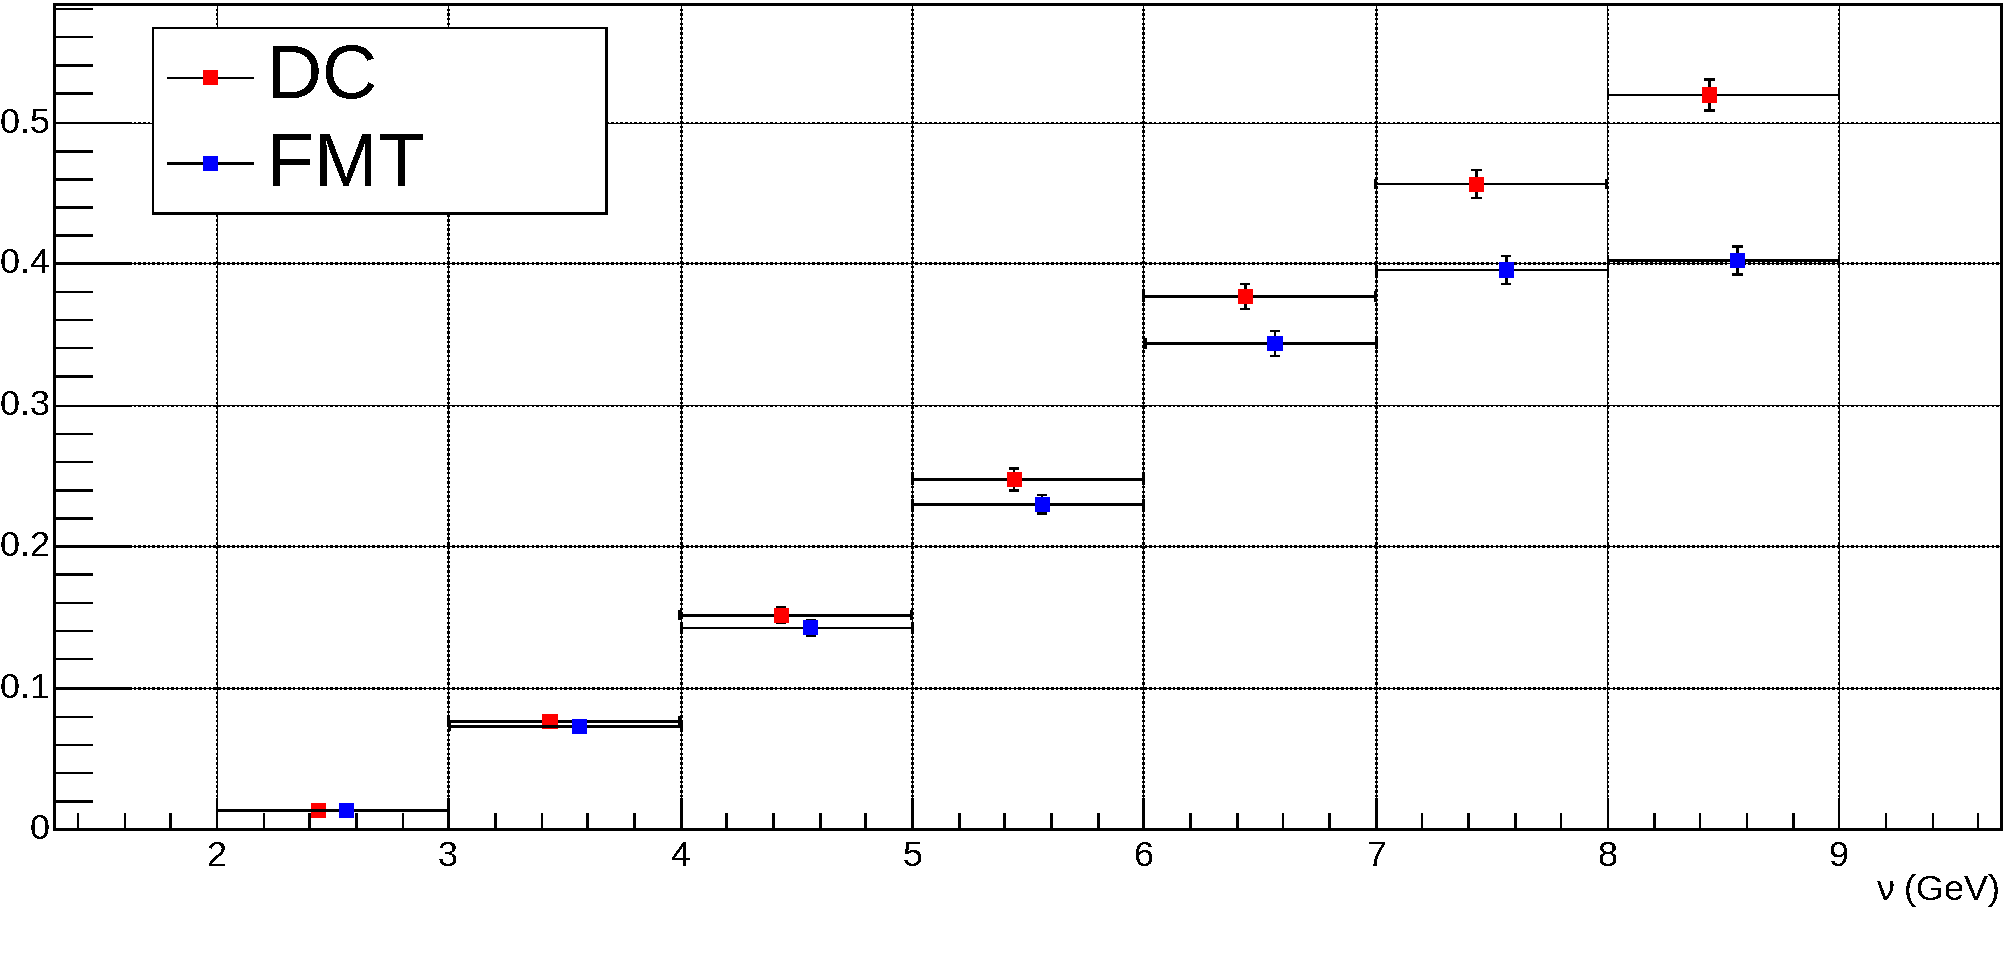
\includegraphics[width=\textwidth]{21nu_acc.pdf}
            \caption{$\nu$ acceptance.}
            \label{fig::14.21::nu_acc}
        \end{subfigure}
        \caption[$e^-$ variables acceptance]
        {$e^-$ variables acceptance.
        $\nu$ is integrated in \ref{fig::14.21::q2_acc}, and $Q^2$ is integrated in \ref{fig::14.21::nu_acc}.
        The bin markers are slightly shifted in $x$ to improve legibility.}
        \floatfoot{Source: Own elaboration, using the \href{https://github.com/bleaktwig/clas12-rge-analysis}{clas12-rge-analysis} software.}
        \label{fig::14.21::electron_acc}
    \end{figure}

    \begin{figure}
        \centering
        % phi vs. theta.
        \begin{subfigure}[b]{\textwidth}
            \centering
            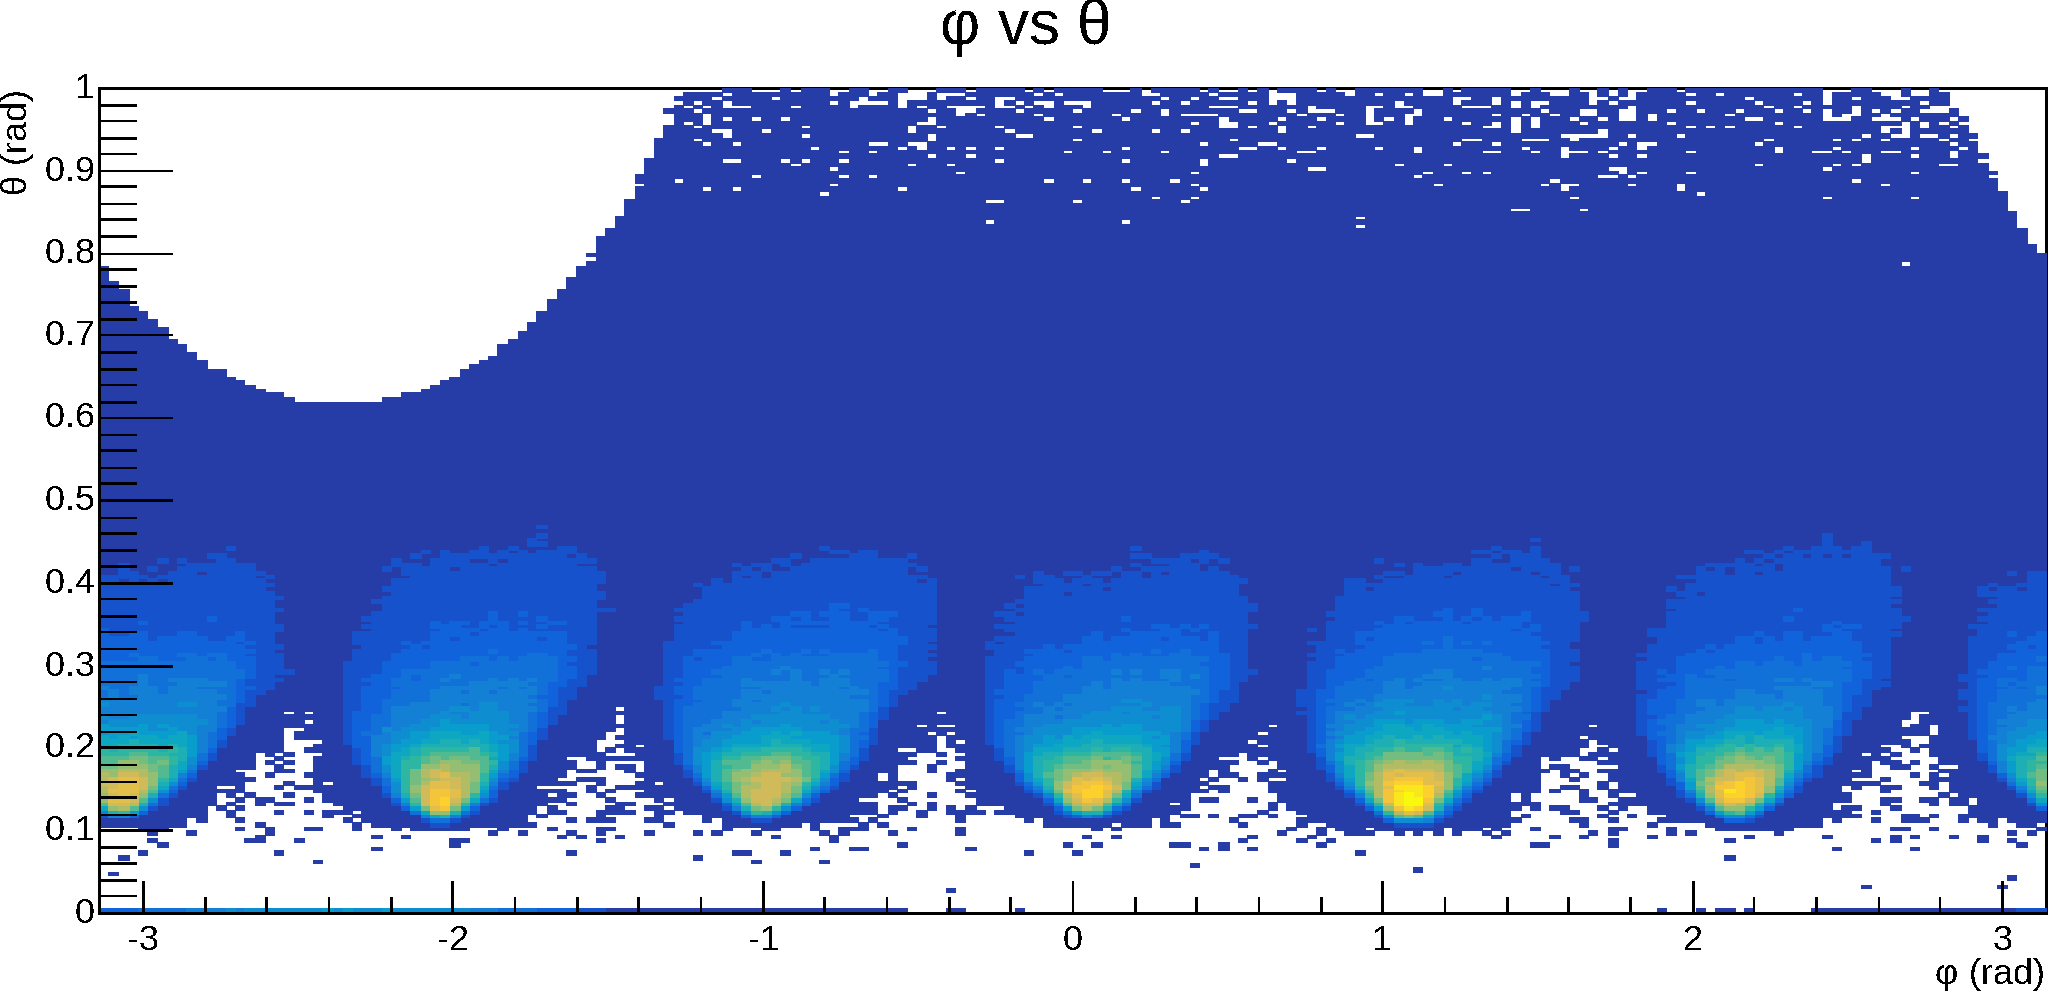
\includegraphics[width=\textwidth]{21phi_theta_neg.pdf}
            \caption[$\phi$ vs. $\theta$ for negative particles]
            {$\phi$ vs. $\theta$ for negative particles detected by DC.}
            \label{fig::14.21::phi_theta_neg}
        \end{subfigure}
        % theta.
        \begin{subfigure}[b]{\textwidth}
            \centering
            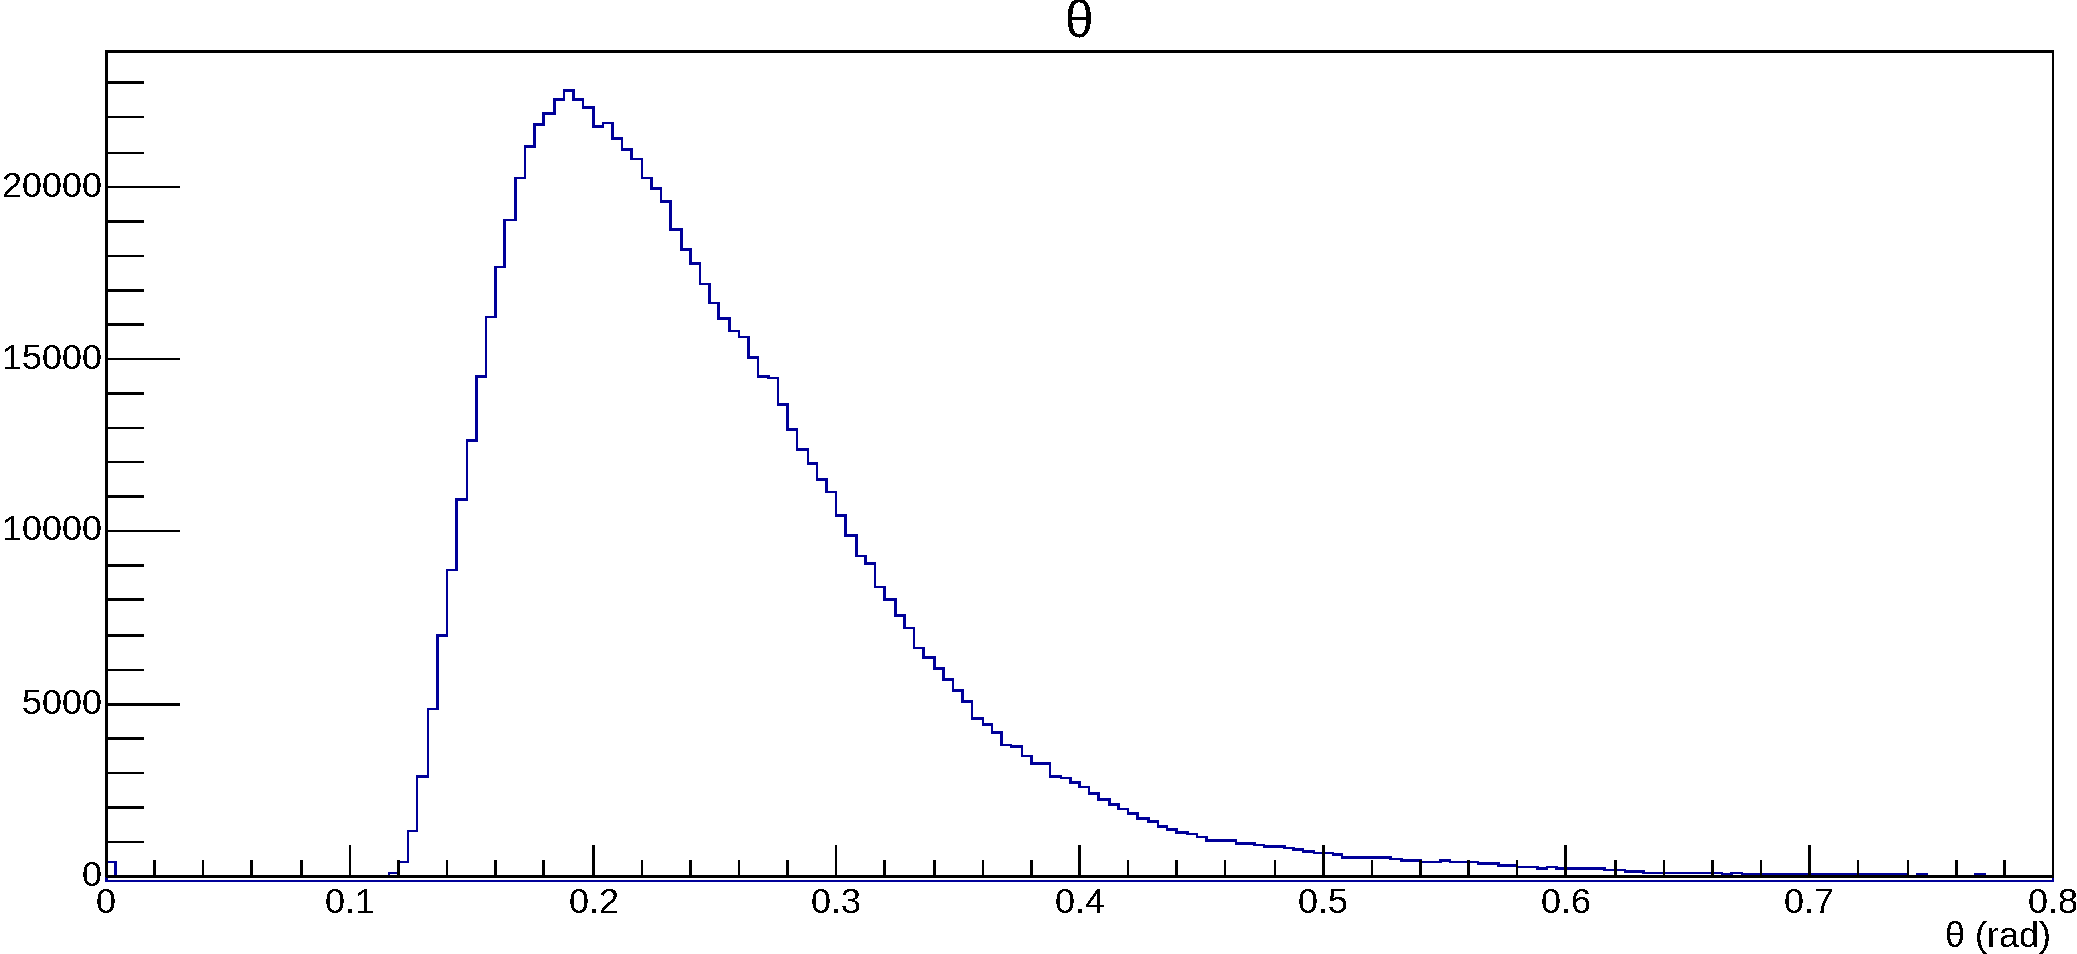
\includegraphics[width=\textwidth]{21theta_neg.pdf}
            \caption[$\theta$ for negative particles]
            {$\theta$ for negative particles detected by DC.}
            \label{fig::14.21::theta_neg}
        \end{subfigure}
        \caption[$\theta$ study for negative particles]
        {$\theta$ study for negative particles.
        Simulated RG-F target.}
        \floatfoot{Source: Own elaboration, using the \href{https://github.com/bleaktwig/clas12-rge-analysis}{clas12-rge-analysis} software.}
        \label{fig::14.21::theta_study_neg}
    \end{figure}

    % Q2.
    In Equation \eqref{eq::13.23::q2}, it can be observed that $Q^2$ has a quadratic dependence on the scattering angle $\theta_C$ of the scattered electrons.%, particularly for small angles.
    Hence, it is important to understand the $\theta$ acceptance of CLAS12 in order to distinguish the geometric effect related to $\theta$ from the inherent $Q^2$ acceptance of the FD.
    Figure \ref{fig::14.21::theta_study_neg} illustrates this dependence for negative particles.

    The triangular shape of each DC sector, combined with the inbending tracks resulting from the negative torus field, leads to a significantly low acceptance at low $\theta$ angles.
    When integrating across $\phi$, this results in a low $\theta$ efficiency for $\theta \lsim 0.15$ radians.
    Referring back to the $Q^2$ plot in Figure \ref{fig::14.21::q2_acc}, the decrease in $Q^2$ acceptance between 1 and 4 $GeV^2$ can be clearly attributed to this geometric effect, which is purely of a geometric nature.

    % nu
    On the other hand, since $\nu$ does not exhibit a direct correlation with $\theta_C$ (as indicated by Equation \eqref{eq::13.23::nu}), we can assume that the acceptance observed in Figure \ref{fig::14.21::nu_acc} is intrinsic to the detector.

    % !TEX root = ../main.tex
\subsubsection{Hadronic Variables}
\label{14.22::hadronic_variables}
    Next, we'll look at $z_h$, $p_T^2$, and $\phi_{PQ}$ acceptances for $e^-\pi^+$ and $e^-\pi^-$.
    It's worth noting that these acceptances are lower than those for electron variables.
    This is to be expected, since they require both the trigger electron and at least one hadron to be accepted by the detector, as is seen also on their efficiencies, as presented in Table \ref{tab::14.14::fmt_efficiency_study}

    \textbf{TODO. Say something?}

    We can see $z_h$ acceptance in Figure \textbf{TODO}, where... (TODO).

    Next, $p_T^2$ acceptance is presented in Figure \textbf{TODO}, where we see that... (TODO).

    Finally, $\phi_{PQ}$ acceptance is studied in Figure \textbf{TODO}.
    Here, we see... (TODO).

    % zh.
    \begin{figure}
        \centering
        % pi+.
        \begin{subfigure}[b]{0.49\textwidth}
            \centering
            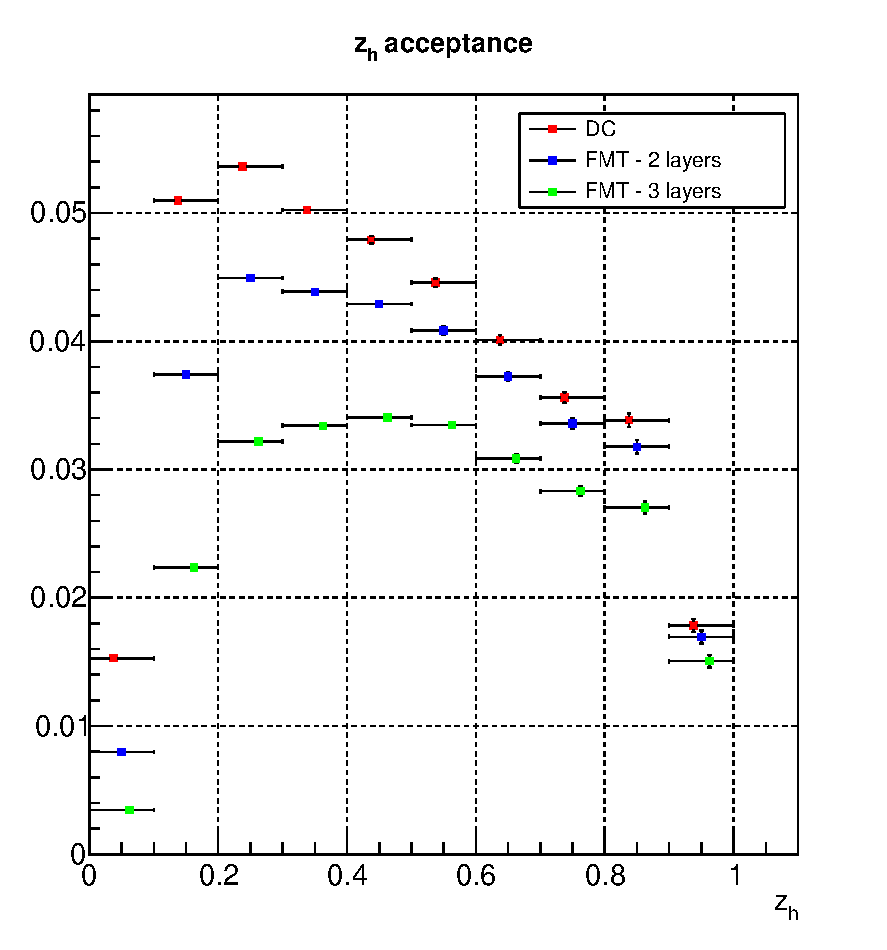
\includegraphics[width=\textwidth]{22zh_acc_211.pdf}
            \caption{$z_h$ acceptance for $e^-\pi^+$.}
            \label{fig::14.22::zh_acc_211}
        \end{subfigure}
        \hfill
        % pi-.
        \begin{subfigure}[b]{0.49\textwidth}
            \centering
            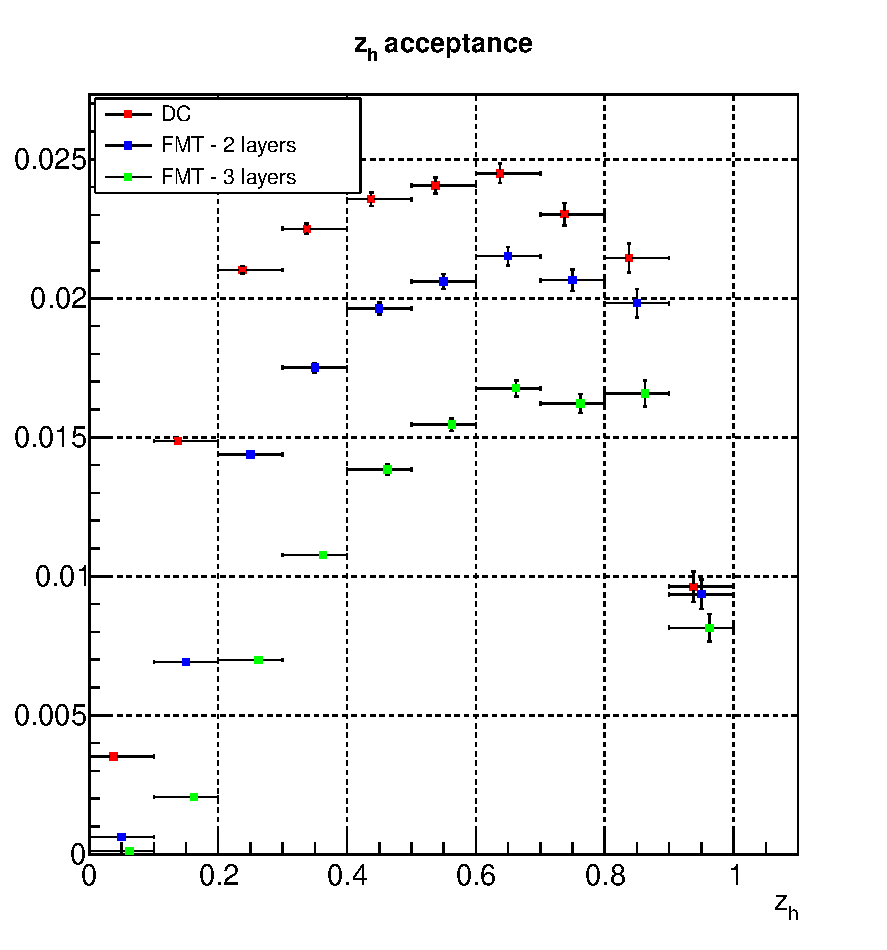
\includegraphics[width=\textwidth]{22zh_acc_-211.pdf}
            \caption{$z_h$ acceptance for $e^-\pi^-$.}
            \label{fig::14.22::zh_acc_-211}
        \end{subfigure}
        \caption[$z_h$ acceptance.]{$z_h$ acceptance for $e^-\pi^+$ and $e^-\pi^-$.
        All electron and other hadronic variables are integrated in both plots.
        The bin markers are slightly shifted in $x$ to improve legibility.
        Source: Own elaboration, using the \href{https://github.com/bleaktwig/clas12-rge-analysis}{clas12-rge-analysis} software.}
        \label{fig::14.22::zh_acc}
    \end{figure}

    % Pt2.
    \begin{figure}
        \centering
        % pi+.
        \begin{subfigure}[b]{0.49\textwidth}
            \centering
            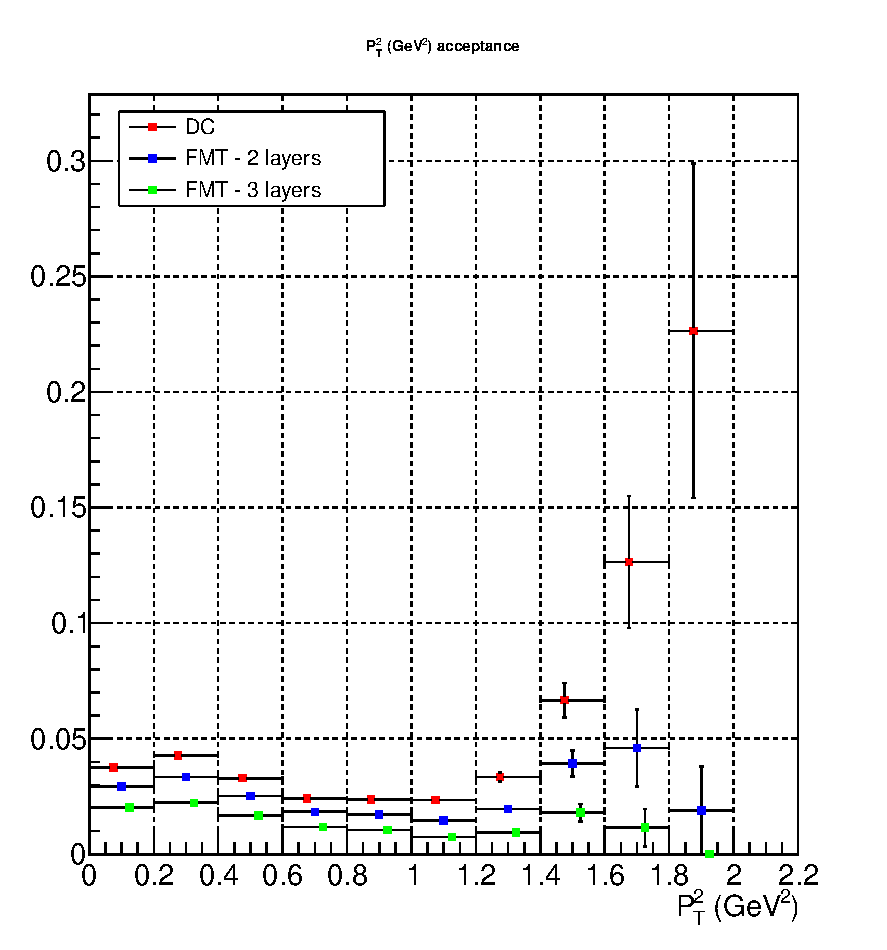
\includegraphics[width=\textwidth]{22pt2_acc_211.pdf}
            \caption{$p_T^2$ acceptance for $e^-\pi^+$.}
            \label{fig::14.22::pt2_acc_211}
        \end{subfigure}
        \hfill
        % pi-.
        \begin{subfigure}[b]{0.49\textwidth}
            \centering
            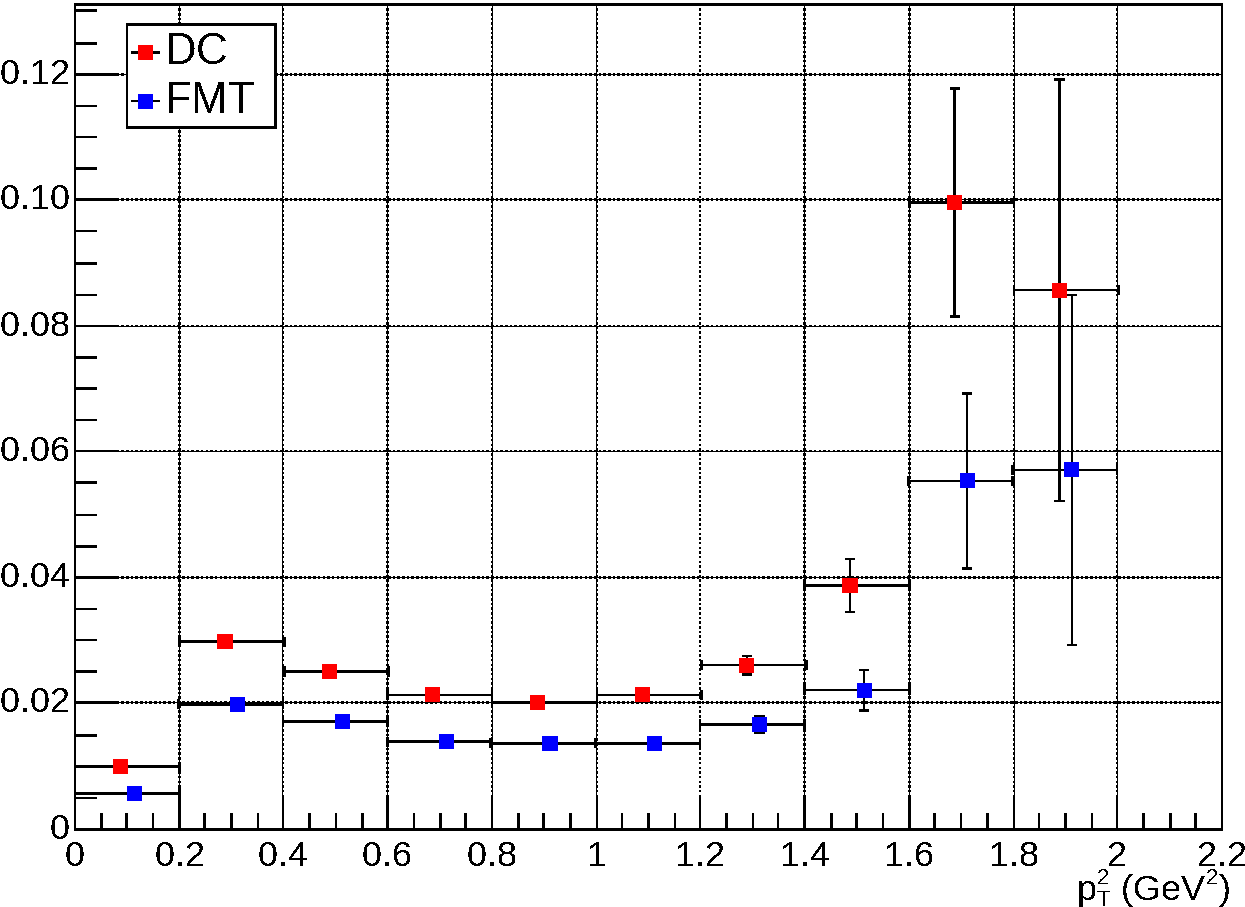
\includegraphics[width=\textwidth]{22pt2_acc_-211.pdf}
            \caption{$p_T^2$ acceptance for $e^-\pi^-$.}
            \label{fig::14.22::pt2_acc_-211}
        \end{subfigure}
        \caption[$p_T^2$ acceptance.]{$p_T^2$ acceptance for $e^-\pi^+$ and $e^-\pi^-$.
        All electron and other hadronic variables are integrated in both plots.
        The bin markers are slightly shifted in $x$ to improve legibility.
        Source: Own elaboration, using the \href{https://github.com/bleaktwig/clas12-rge-analysis}{clas12-rge-analysis} software.}
        \label{fig::14.22::pt2_acc}
    \end{figure}

    % phipq.
    \begin{figure}
        \centering
        % pi+.
        \begin{subfigure}[b]{0.49\textwidth}
            \centering
            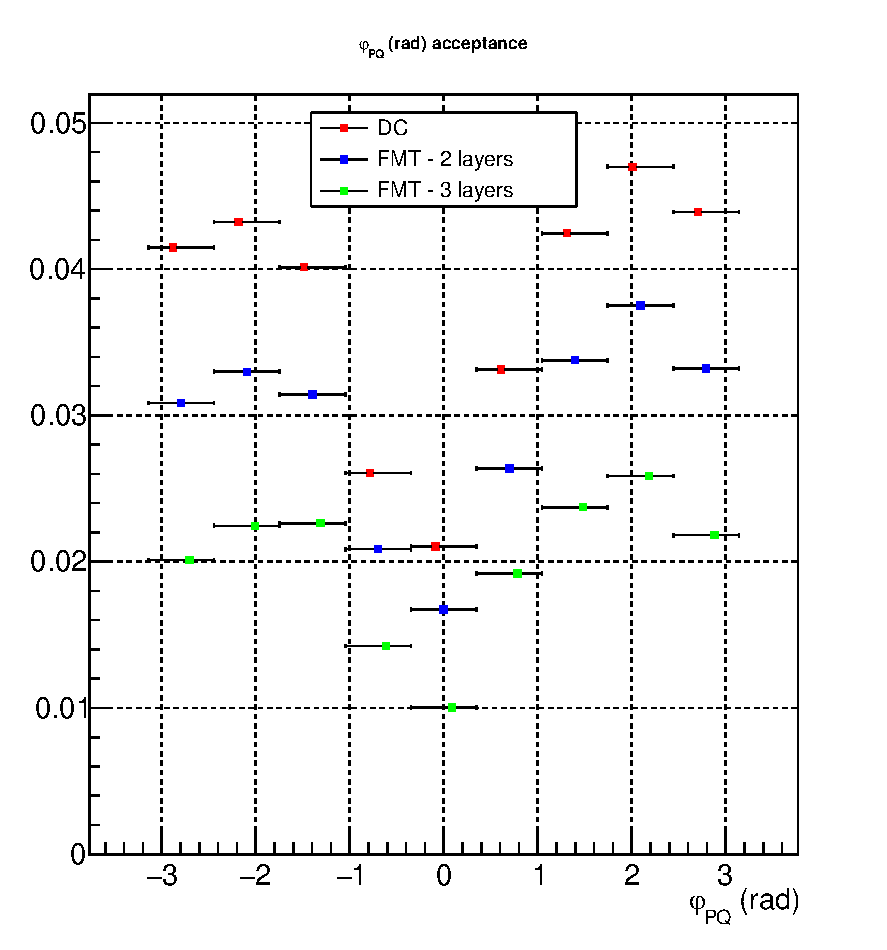
\includegraphics[width=\textwidth]{22phipq_acc_211.pdf}
            \caption{$\phi_{PQ}$ acceptance for $e^-\pi^+$.}
            \label{fig::14.22::phipq_acc_211}
        \end{subfigure}
        \hfill
        % pi-.
        \begin{subfigure}[b]{0.49\textwidth}
            \centering
            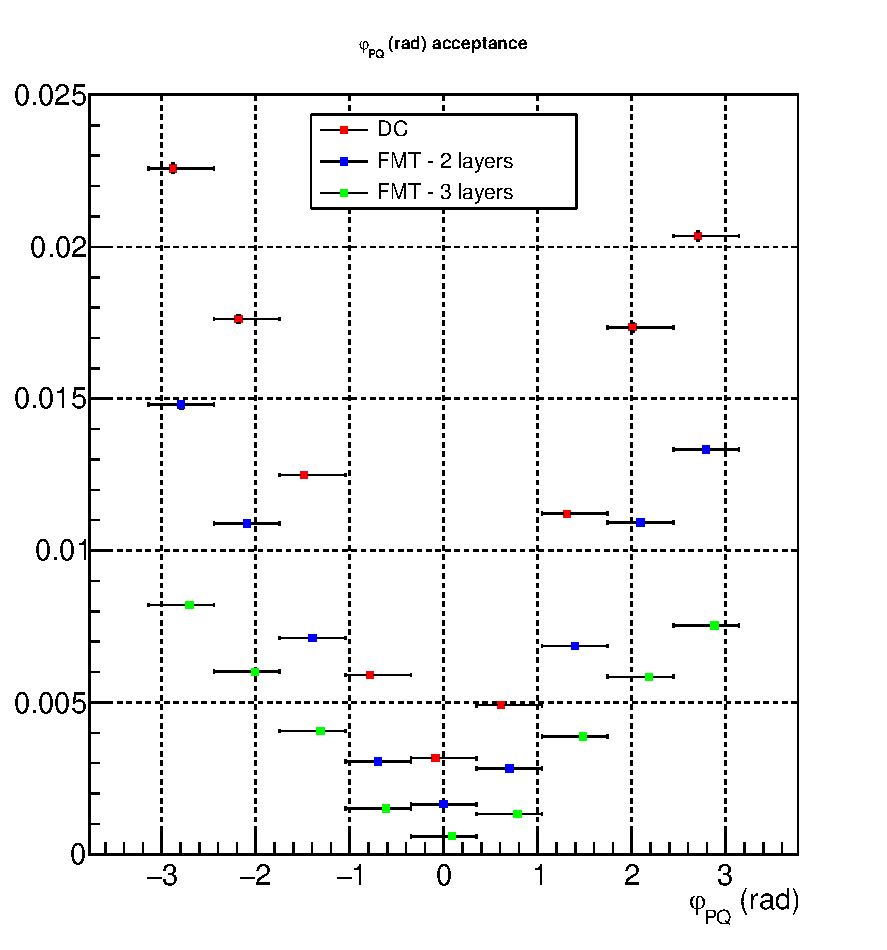
\includegraphics[width=\textwidth]{22phipq_acc_-211.pdf}
            \caption{$\phi_{PQ}$ acceptance for $e^-\pi^-$.}
            \label{fig::14.22::phipq_acc_-211}
        \end{subfigure}
        \caption[$\phi_{PQ}$ acceptance.]{$\phi_{PQ}$ acceptance for $e^-\pi^+$ and $e^-\pi^-$.
        All electron and other hadronic variables are integrated in both plots.
        The bin markers are slightly shifted in $x$ to improve legibility.
        Source: Own elaboration, using the \href{https://github.com/bleaktwig/clas12-rge-analysis}{clas12-rge-analysis} software.}
        \label{fig::14.22::phipq_acc}
    \end{figure}


% --+ Plots +-------------------------------------------------------------------
    % \begin{figure}[hbtp]
    %     % Q2.
    %     \begin{subfigure}{.5\textwidth}
    %         \centering
    %         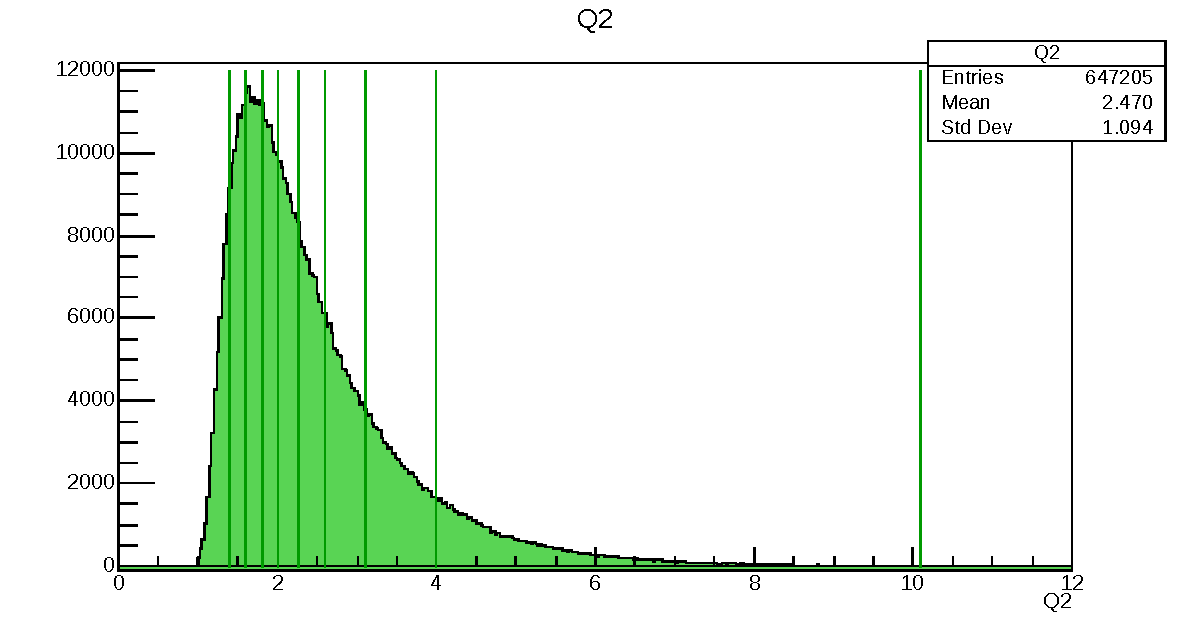
\includegraphics[width=\linewidth]{13dataanalysis/img/40_accbins_q2.pdf}
    %         % \caption{$Q^2$ bins.}
    %         \label{fig::acc_corr_bins_q2}
    %     \end{subfigure}
    %     \begin{subfigure}{.5\textwidth}
    %         \centering
    %         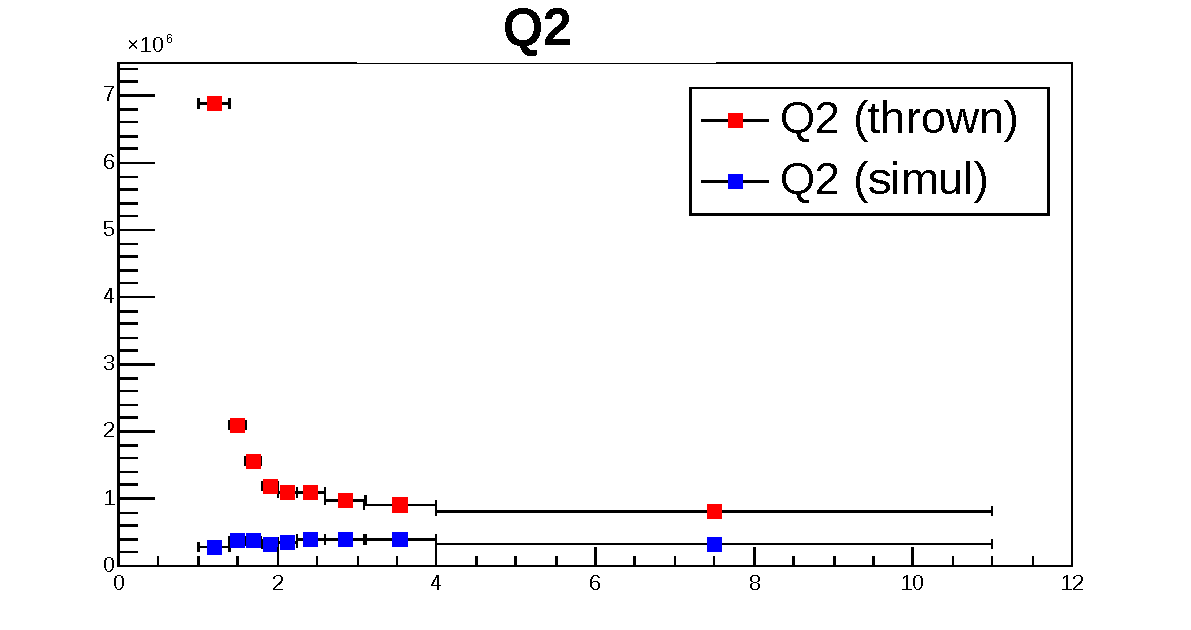
\includegraphics[width=\linewidth]{13dataanalysis/img/40_acccorr_q2.pdf}
    %         % \caption{$Q^2$ acceptance correction results.}
    %         \label{fig::acc_corr_q2}
    %     \end{subfigure}
    %
    %     % nu.
    %     \begin{subfigure}{.5\textwidth}
    %         \centering
    %         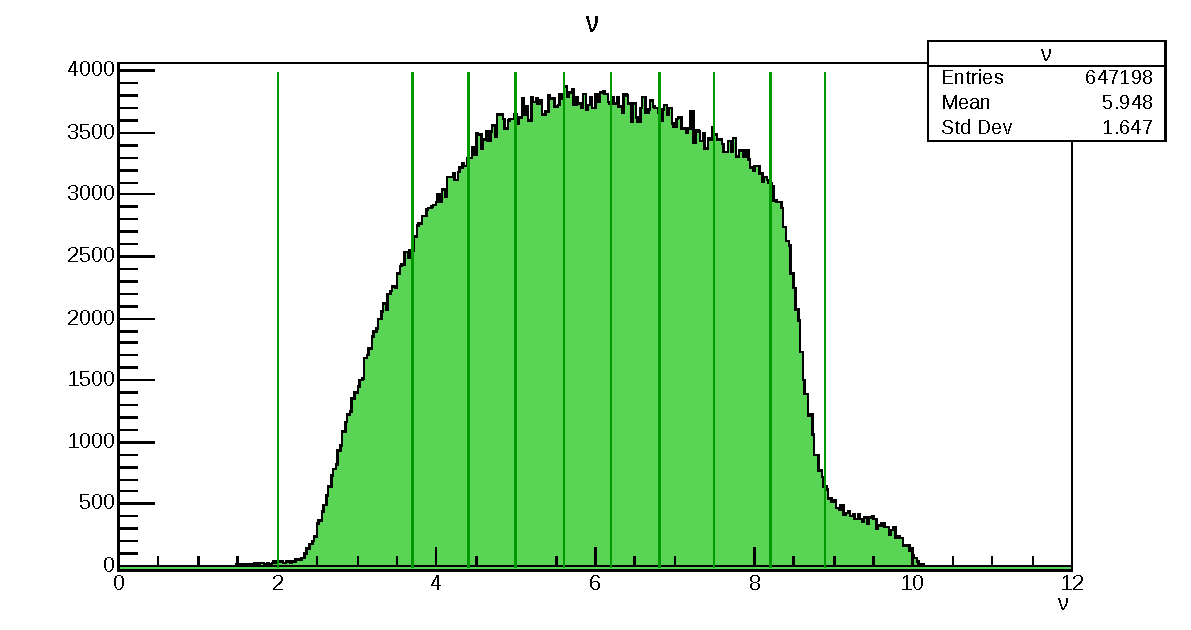
\includegraphics[width=\linewidth]{13dataanalysis/img/40_accbins_nu.pdf}
    %         % \caption{$\nu$ bins.}
    %         \label{fig::acc_corr_bins_nu}
    %     \end{subfigure}
    %     \begin{subfigure}{.5\textwidth}
    %         \centering
    %         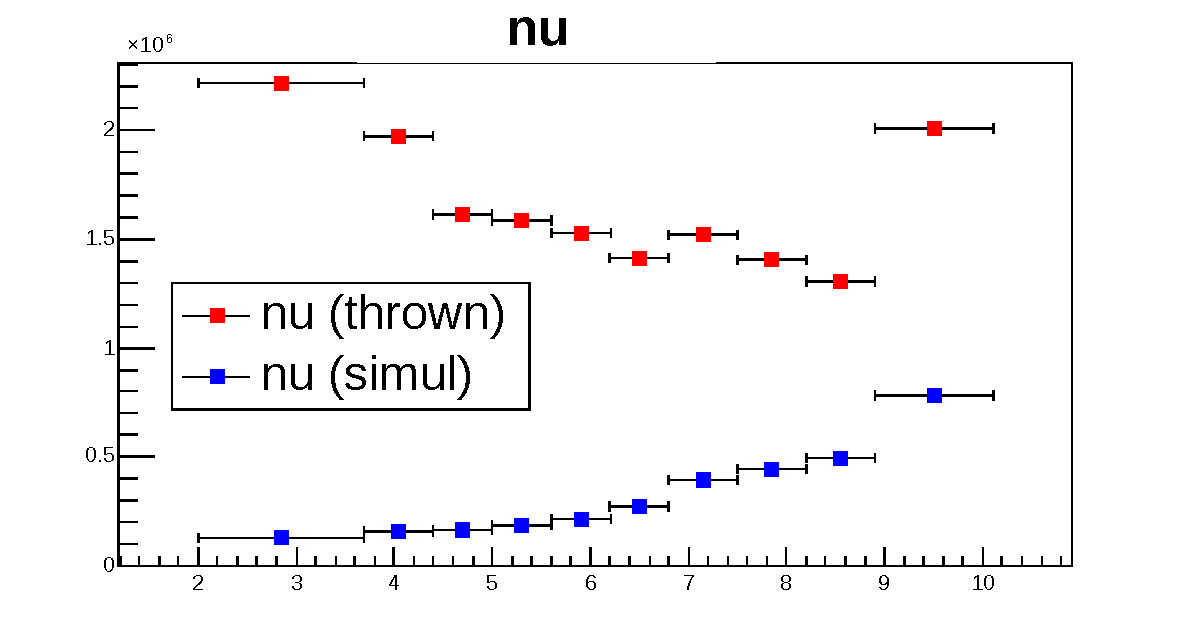
\includegraphics[width=\linewidth]{13dataanalysis/img/40_acccorr_nu.pdf}
    %         % \caption{$\nu$ acceptance correction results.}
    %         \label{fig::acc_corr_nu}
    %     \end{subfigure}
    %
    %     % zh.
    %     \begin{subfigure}{.5\textwidth}
    %         \centering
    %         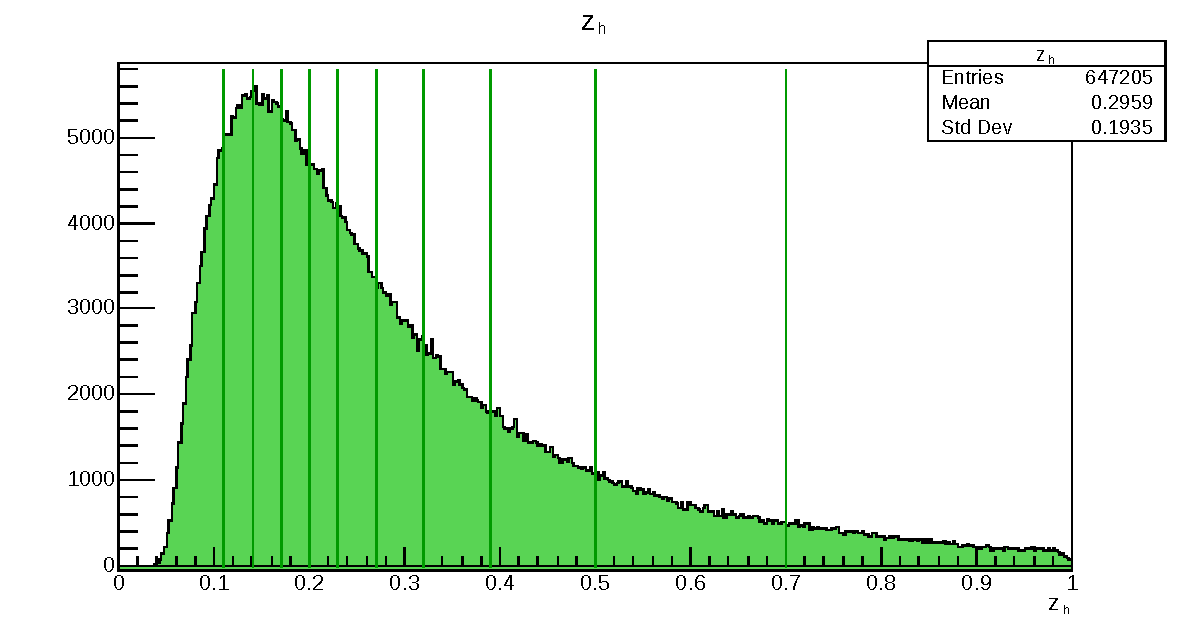
\includegraphics[width=\linewidth]{13dataanalysis/img/40_accbins_zh.pdf}
    %         % \caption{$z_h$ bins.}
    %         \label{fig::acc_corr_bins_zh}
    %     \end{subfigure}
    %     \begin{subfigure}{.5\textwidth}
    %         \centering
    %         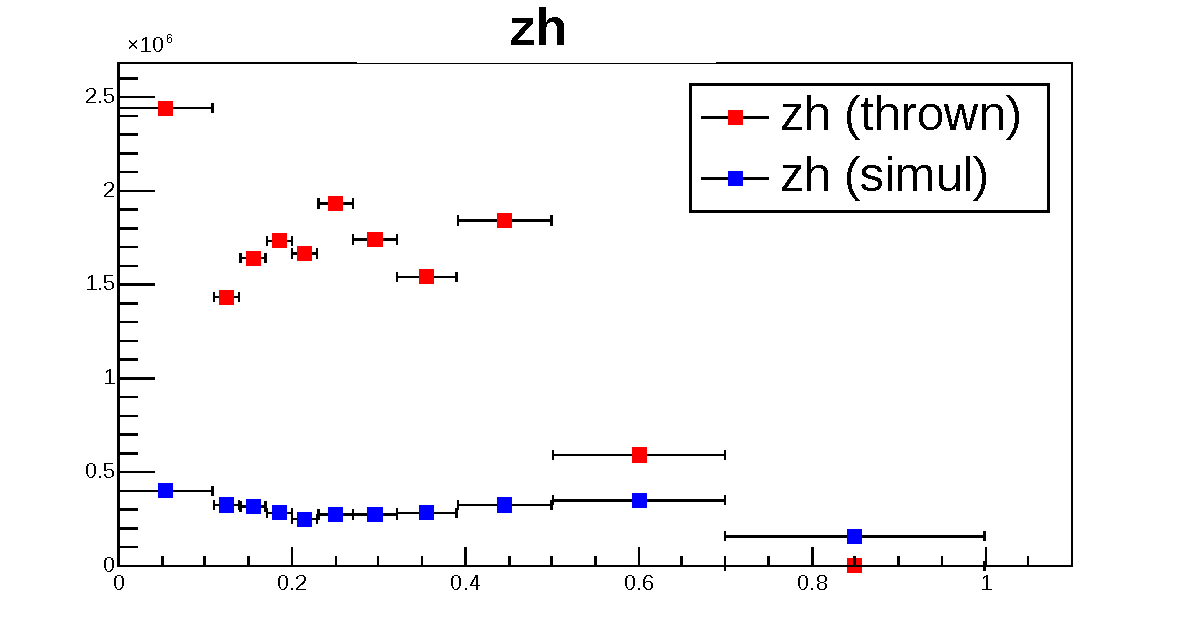
\includegraphics[width=\linewidth]{13dataanalysis/img/40_acccorr_zh.pdf}
    %         % \caption{$z_h$ acceptance correction results.}
    %         \label{fig::acc_corr_zh}
    %     \end{subfigure}
    %
    %     % PT2.
    %     \begin{subfigure}{.5\textwidth}
    %         \centering
    %         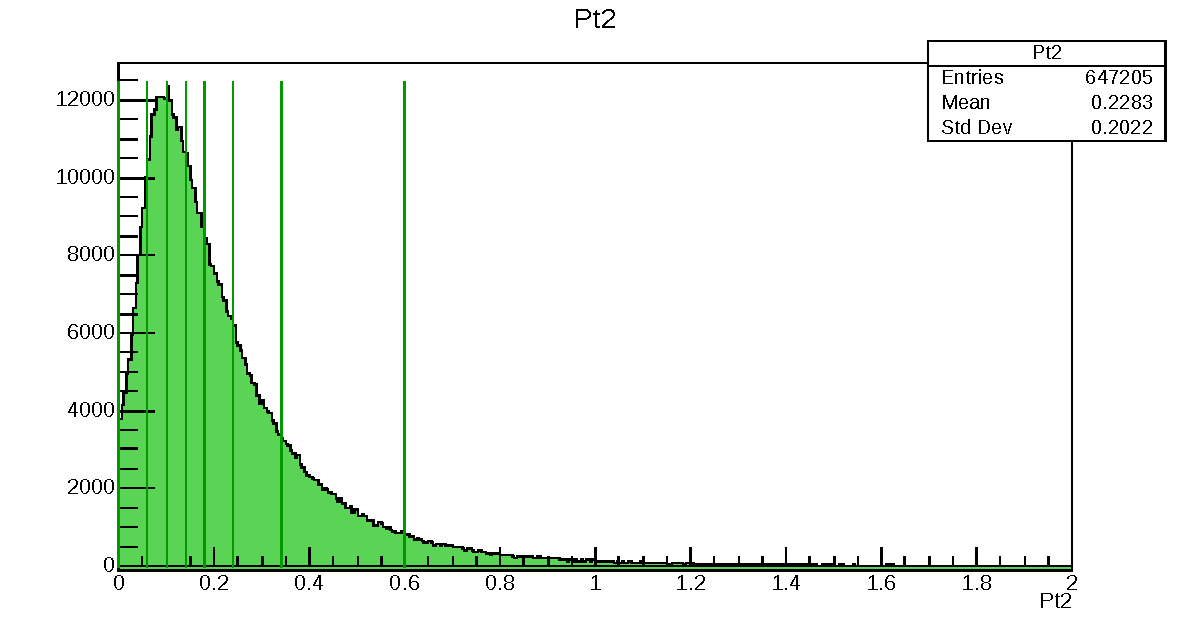
\includegraphics[width=\linewidth]{13dataanalysis/img/40_accbins_pt2.pdf}
    %         % \caption{$P_T^2$ bins.}
    %         \label{fig::acc_corr_bins_pt2}
    %     \end{subfigure}
    %     \begin{subfigure}{.5\textwidth}
    %         \centering
    %         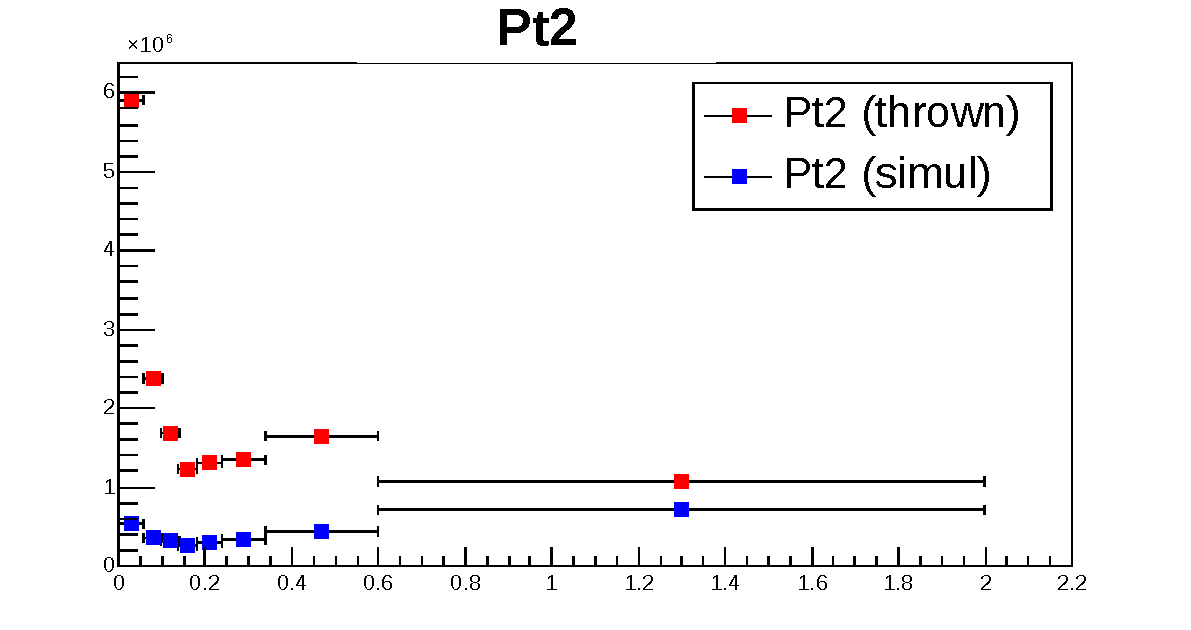
\includegraphics[width=\linewidth]{13dataanalysis/img/40_acccorr_pt2.pdf}
    %         % \caption{$P_T^2$ acceptance correction results.}
    %         \label{fig::acc_corr_pt2}
    %     \end{subfigure}
    %
    %     % phi_PQ.
    %     \begin{subfigure}{.5\textwidth}
    %         \centering
    %         \includegraphics[width=\linewidth]{13dataanalysis/img/40_accbins_phipq.pdf}
    %         % \caption{$\phi_{PQ}$ bins.}
    %         \label{fig::acc_corr_bins_phipq}
    %     \end{subfigure}
    %     \begin{subfigure}{.5\textwidth}
    %         \centering
    %         \includegraphics[width=\linewidth]{13dataanalysis/img/40_acccorr_phipq.pdf}
    %         % \caption{$\phi_{PQ}$ acceptance correction results.}
    %         \label{fig::acc_corr_phipq}
    %     \end{subfigure}
    %
    %     \caption[Acceptance correction results.]{Acceptance correction results for the kinematical variables $Q^2$, $\nu$, $z_h$, $p_T^2$, and $\phi_{PQ}$. On the left plots, the acceptance correction bin edges are shown. On the right, the number of thrown (in red) and simulated (in blue) entries for each of the variables is shown. All other variables are integrated for each plot.}
    %     \label{fig::acc_corr}
    % \end{figure}

    % !TEX root = ../main.tex
\subsection{Study Results}
\label{14.30::study_results}
    % TODO. Explain binning scheme selected.

    % TODO. Explain how "good" bins will be selected.
    %   * TODO. First criterium for selecting a good bin is maximising the phase space of each variable.
    %   * TODO. Then, the second criterium is maximising the statistics of that variable.
    %   * NOTE. As Hayk if I should use the results without acceptance correction to deduce the statistics?

    % statistical error estimation.
    The total statistical error on the acceptance corrected result $e_\text{corr}$ needs to consider both the statistical error of the measurements $e_\text{meas}$ and that of the acceptance correction $e_\text{acc}$.
    The former is purely statistical in nature, and is thus given by
    \begin{equation*}
        e_\text{meas} = \frac{\delta y_\text{meas}}{y_\text{meas}},
    \end{equation*}
    and the latter was derived in Equation \eqref{eq::14.20::acc_error}.

    Considering the fact that $e_\text{meas}$ comes purely from experimental data and $e_\text{acc}$ comes purely from simulation, they are completely uncorrelated.
    Thus, we can estimate the total statistical error of the acceptance corrected result as the quadratic addition of the two, or
    \begin{equation*}
        e_\text{corr} = \sqrt{e_\text{meas}^2 + e_\text{acc}^2}.
    \end{equation*}

    % TODO. systematic error "estimation".
    %   * TODO. Ask Raffaella for a reference about the "average" systematic error we should consider.

    % resulting plots.
    Each of the acceptance corrected DIS variables can be seen separated in $v_z$ bins in Figures \ref{fig::14.30::q2_vz} to \ref{fig::14.30::phipq_vz_-211}.
    The electron variables distributions, $Q^2$ and $\nu$, can be seen in Figures \ref{fig::14.30::q2_vz} and \ref{fig::14.30::nu_vz} respectively.
    Then, $z_h$ can be observed in Figures \ref{fig::14.30::zh_211_vz} for $e^-\pi^+$, and in \ref{fig::14.30::zh_-211_vz} for $e^-\pi^-$.
    $p_T^2$ for $e^-\pi^+$ can be seen in Figure \ref{fig::14.30::pt2_211_vz}, and for $e^-\pi^-$ in Figure \ref{fig::14.30::pt2_-211_vz}.
    At last, the $\phi_{PQ}$ distributions for $e^-\pi^+$ can be observed in Figure \ref{fig::14.30::phipq_211_vz}, while for $e^-\pi^-$ in Figure \ref{fig::14.30::phipq_-211_vz}.

    % Q2.
    \begin{figure}
        \centering
        \includegraphics[width=\textwidth]{30q2_vz.png}
        \caption[Acceptance-corrected $Q^2$ separated in $v_z$ bins, run 12016]
        {Acceptance-corrected $Q^2$ detected by DC and FMT, separated in $v_z$ bins.
        Run 12016.}
        \floatfoot{Source: Own elaboration, using the \href{https://github.com/bleaktwig/clas12-rge-analysis}{clas12-rge-analysis} software.}
        \label{fig::14.30::q2_vz}
    \end{figure}

    % nu.
    \begin{figure}
        \centering
        \includegraphics[width=\textwidth]{30nu_vz.png}
        \caption[Acceptance-corrected $\nu$ separated in $v_z$ bins, run 12016]
        {Acceptance-corrected $\nu$ detected by DC and FMT, separated in $v_z$ bins.
        Run 12016.}
        \floatfoot{Source: Own elaboration, using the \href{https://github.com/bleaktwig/clas12-rge-analysis}{clas12-rge-analysis} software.}
        \label{fig::14.30::nu_vz}
    \end{figure}

    % zh.
    \begin{figure}
        \centering
        \includegraphics[width=\textwidth]{30zh_vz_211.png}
        \caption[Acceptance-corrected $z_h$ for $e^-\pi^+$ separated in $v_z$ bins, run 12016]
        {Acceptance-corrected $z_h$ for $e^-\pi^+$ detected by DC and FMT, separated in $v_z$ bins.
        Run 12016.}
        \floatfoot{Source: Own elaboration, using the \href{https://github.com/bleaktwig/clas12-rge-analysis}{clas12-rge-analysis} software.}
        \label{fig::14.30::zh_211_vz}
    \end{figure}

    \begin{figure}
        \centering
        \includegraphics[width=\textwidth]{30zh_vz_-211.png}
        \caption[Acceptance-corrected $z_h$ for $e^-\pi^-$ separated in $v_z$ bins, run 12016]
        {Acceptance-corrected $z_h$ for $e^-\pi^-$ detected by DC and FMT, separated in $v_z$ bins.
        Run 12016.}
        \floatfoot{Source: Own elaboration, using the \href{https://github.com/bleaktwig/clas12-rge-analysis}{clas12-rge-analysis} software.}
        \label{fig::14.30::zh_-211_vz}
    \end{figure}

    % pt2.
    \begin{figure}
        \centering
        \includegraphics[width=\textwidth]{30pt2_vz_211.png}
        \caption[Acceptance-corrected $p_T^2$ for $e^-\pi^+$ separated in $v_z$ bins, run 12016]
        {Acceptance-corrected $p_T^2$ for $e^-\pi^+$ detected by DC and FMT, separated in $v_z$ bins.
        Run 12016.}
        \floatfoot{Source: Own elaboration, using the \href{https://github.com/bleaktwig/clas12-rge-analysis}{clas12-rge-analysis} software.}
        \label{fig::14.30::pt2_211_vz}
    \end{figure}

    \begin{figure}
        \centering
        \includegraphics[width=\textwidth]{30pt2_vz_-211.png}
        \caption[Acceptance-corrected $p_T^2$ for $e^-\pi^-$ separated in $v_z$ bins, run 12016]
        {Acceptance-corrected $p_T^2$ for $e^-\pi^-$ detected by DC and FMT, separated in $v_z$ bins.
        Run 12016.}
        \floatfoot{Source: Own elaboration, using the \href{https://github.com/bleaktwig/clas12-rge-analysis}{clas12-rge-analysis} software.}
        \label{fig::14.30::pt2_-211_vz}
    \end{figure}

    % phipq.
    \begin{figure}
        \centering
        \includegraphics[width=\textwidth]{30phipq_vz_211.png}
        \caption[Acceptance-corrected $\phi_{PQ}$ for $e^-\pi^+$ separated in $v_z$ bins, run 12016]
        {Acceptance-corrected $\phi_{PQ}$ for $e^-\pi^+$ detected by DC and FMT, separated in $v_z$ bins.
        Run 12016.}
        \floatfoot{Source: Own elaboration, using the \href{https://github.com/bleaktwig/clas12-rge-analysis}{clas12-rge-analysis} software.}
        \label{fig::14.30::phipq_211_vz}
    \end{figure}

    \begin{figure}
        \centering
        \includegraphics[width=\textwidth]{30phipq_vz_-211.png}
        \caption[Acceptance-corrected $\phi_{PQ}$ for $e^-\pi^-$ separated in $v_z$ bins, run 12016]
        {Acceptance-corrected $\phi_{PQ}$ for $e^-\pi^-$ detected by DC and FMT, separated in $v_z$ bins.
        Run 12016.}
        \floatfoot{Source: Own elaboration, using the \href{https://github.com/bleaktwig/clas12-rge-analysis}{clas12-rge-analysis} software.}
        \label{fig::14.30::phipq_-211_vz}
    \end{figure}

    % TODO. draw conclusions.

    % TODO. Mention nu and zh and how they shouldn't (and don't) show any dependence.

    % TODO. Metnion and show that Q2, pt2, and phiPQ show dependence on theta angle.

    % TODO. Decide on a range based on Q2 phase space. Show that the same can be concluded from pt2 and phiPQ, but Q2 is easier to study due to only coming from the e-.
    As can be seen on the figure, the higher end of the variable's phase space is limited for $v_z < -5$ cm, with the effect becoming more pronounced the further upstream we go.
    This effect can be understood by compounding the $\theta$ efficiency for negative particles (see Figure \ref{fig::14.21::theta_study_neg}) and the limited acceptance region of FMT given by Equation \eqref{eq::12.42::fmt_geometry_cut} (see Figure \ref{eq::12.42::vz_vs_theta}): the higher end of $\theta$ becomes limited for lower $v_z$ values.

    With the stated objective of maximising the phase space of each variable, this draws us to set the minimum $v_z$ for the RG-E target to $-5$ cm.
    Furthermore, we can limit the maximum $v_z$ to $10$ cm, since the low values of $\theta$ become limited by the lower end of the FMT's acceptance region.

    % TODO. Decide on a final position based on statistics.


% \subsection{Conclusions}
% TODO. Something something something.
% TODO. Mention issue of large systematic errors (~10%) not considered in the work.
%   * TODO. Ask Raffaella for a reference about the "average" systematic error I should consider.

    \pagebreak

    % --+ Addenda +-------------------------------------------------------------
    \appendix
    \graphicspath{{20appendices/img}}
    % !TEX root = ../main.tex
\section*{Appendices}
\addcontentsline{toc}{section}{Appendices}
\label{20::appendices}
    \renewcommand{\thesubsection}{\Alph{subsection}}
    % !TEX root = ../main.tex
\subsection{Reproducibility}
\label{20.01::reproducibility}
    In order to ensure the reproducibility of the research presented in this thesis, we provide access to all datasets and code used in the development of our study.
    We believe that transparency and accessibility are crucial for scientific integrity and to facilitate further investigations by the research community.

    We encourage interested readers and fellow researchers to access and utilise these resources for the purpose of reproducibility and advancing scientific knowledge.
    Should there be any inquiries or issues regarding the datasets or code, please do not hesitate to contact the author at \href{mailto:bruno.benkel@gmail.com}{\texttt{bruno.benkel@gmail.com}} for further assistance.

    We believe that open access to data and code fosters collaboration, accelerates scientific progress, and ensures the robustness of research findings.
    By making these resources available, we aim to contribute to the collective effort of reproducible and transparent scientific research.

    % --+ Datasets +------------------------------------------------------------
    \paragraph{Datasets}
        Regrettably, there is no website or location to openly share datasets in the \textit{Universidad Técnica Federico Santa María} (UTFSM) or the \textit{Centro Científico Tecnológico de Valparaíso} (CCTVal).
        For readers with access to the JLab farm, all used datasets are available at

        \begin{center}
            \texttt{/work/clas12/users/benkel/thesis-datasets}
        \end{center}

        For individuals who do not have access to the JLab farm, please feel free to contact the author, and we will explore alternative methods to share the relevant datasets.

    % --+ Code +----------------------------------------------------------------
    \paragraph{Code}
        The sources for the code used for data processing, analysis, and generating figures are shared on Table \ref{tab::20.01::code_locations}.
        By providing the code, we aim to enable researchers to replicate our findings, perform additional analyses, or build upon our work.

        \begin{table}[b!]
            \begin{center}
                \begin{tabularx}{0.90\textwidth}{ll}
                    \toprule
                    \textbf{Software}  & \textbf{Link} \\
                    \midrule \midrule
                    RG-E Slow Controls &
                        \href{https://github.com/bleaktwig/rge-epics-support}
                        {\texttt{github.com/bleaktwig/rge-epics-support}} \\
                    \midrule
                    CLAS12 Alignment   &
                        \href{https://github.com/JeffersonLab/clas12alignment}
                        {\texttt{github.com/JeffersonLab/clas12alignment}} \\
                    \midrule
                    thesis-simul       &
                        \href{https://github.com/bleaktwig/thesis-simul}
                        {\texttt{github.com/bleaktwig/thesis-simul}} \\
                    thesis-data        &
                        \href{https://github.com/bleaktwig/thesis-data}
                        {\texttt{github.com/bleaktwig/thesis-data}} \\
                    RG-E Analysis      &
                        \href{https://github.com/bleaktwig/clas12-rge-analysis}
                        {\texttt{github.com/bleaktwig/clas12-rge-analysis}} \\
                    GEMC               &
                        \href{https://github.com/gemc/source}
                        {\texttt{github.com/gemc/source}} \\
                    Coatjava           &
                        \href{https://github.com/JeffersonLab/coatjava}
                        {\texttt{github.com/JeffersonLab/coatjava}} \\
                \bottomrule
            \end{tabularx}
        \end{center}

        \caption{Table with code locations.}
        \label{tab::20.01::code_locations}
    \end{table}

    % !TEX root = ../main.tex
\addcontentsline{toc}{subsection}{RG-F Target Layout}
\label{20.02::rgf_target_layout}
    \incgraph[documentpaper,][width=\paperwidth,height=\paperheight]{20addenda/img/02rgf_target_layout.pdf}
    % TODO. Once done with addenda, change title of pdf to the correct addendum number.

    % !TEX root = ../main.tex
\subsection{FMT Layer Efficiency Error Estimation}
\label{20.03::fmt_layer_efficiency_error_estimation}
    This Appendix presents the Python script described in Section \ref{14.14::efficiency_study}.
    The script utilises the formulae outlined in that section to estimate the errors in the efficiency of the 2-layer and 3-layer tracks.
    It should be noted, as mentioned in the section, that the efficiency $E_{1(2)}$ (referred to as \verb|E12| in the code) was obtained through numerical methods.

    \begin{lstlisting}[language=Python]
    import sys
    def printf(format, *args):
        sys.stdout.write(format % args)
    def f_E13(E3):
        return E3**(1/3)
    def f_E1(E12, E13):
        return (4*E12 + E13)/5
    def f_dE12(E1, E12):
        return abs(E1 - E12)
    def f_dE13(E1, E13):
        return abs(E1 - E13)
    def f_dE2(E12, dE12):
        return (6*E12 - 9*E12**2) * dE12
    def f_dE3(E13, dE13):
        return 3*E13**2 * dE13

    # Input.
    #      Run 12933.                    Run 12016.
    E2  = [.251,.065,.056,.375,.137,.142,.327,.111,.089,.537,.280,.295]
    E3  = [.056,.003,.003,.085,.007,.007,.099,.010,.009,.164,.027,.029]
    E12 = [.306,.157,.144,.402,.239,.244,.339,.206,.180,.497,.364,.377]

    # Run functions.
    E13  = list(map(f_E13,  E3))
    E1   = list(map(f_E1,   E12, E13))
    dE12 = list(map(f_dE12, E1,  E12))
    dE13 = list(map(f_dE13, E1,  E13))
    dE2  = list(map(f_dE2,  E12, dE12))
    dE3  = list(map(f_dE3,  E13, dE13))

    # Print.
    print("dE2:")
    for i in dE2:
        printf("%5.1f,", 100*i)
    print("dE3:")
    for i in dE3:
        printf("%5.1f,", 100*i)
    \end{lstlisting}

    % !TEX root = ../main.tex
\subsection{DIS plots in $v_z$ bins}
\label{20.04::dis_vz_plots}
    In Section \ref{14.31::phase_space_study}, we presented the acceptance-corrected DIS variables separated into $v_z$ bins.
    In this Appendix, we provide the same distributions without applying the acceptance correction.
    The statistics are considerably lower in $v_z$ bins characterised by low acceptance, such as $v_z > 10$ cm.
    This effect is more pronounced for the hadronic variables, as one would expect.
    Moreover, the correction noticeably alters the shape of certain distributions, bringing them closer to the expected theoretical behaviour.
    A clear illustration of this can be observed in the disparity of $Q^2$ depicted in Figures \ref{fig::14.31::q2_vz} and \ref{fig::20.04::q2_vz}, as well as in the dissimilarity of $z_h$ demonstrated in Figures \ref{fig::14.31::zh_211_vz} and \ref{fig::20.04::zh_211_vz}.

    % Q2.
    \begin{figure}
        \centering
        \includegraphics[width=\textwidth]{04q2_vz.png}
        \caption[$Q^2$ separated in $v_z$ bins]
        {$Q^2$ detected by DC and FMT, separated in $v_z$ bins.
        Run 12016.
        The bin markers are slightly shifted in $x$ to improve legibility.}
        \floatfoot{Source: Own elaboration, using the \href{https://github.com/bleaktwig/clas12-rge-analysis}{clas12-rge-analysis} software.}
        \label{fig::20.04::q2_vz}
    \end{figure}

    % nu.
    \begin{figure}
        \centering
        \includegraphics[width=\textwidth]{04nu_vz.png}
        \caption[$\nu$ separated in $v_z$ bins]
        {$\nu$ detected by DC and FMT, separated in $v_z$ bins.
        Run 12016.
        The bin markers are slightly shifted in $x$ to improve legibility.}
        \floatfoot{Source: Own elaboration, using the \href{https://github.com/bleaktwig/clas12-rge-analysis}{clas12-rge-analysis} software.}
        \label{fig::20.04::nu_vz}
    \end{figure}

    % zh.
    \begin{figure}
        \centering
        \includegraphics[width=\textwidth]{04zh_vz_211.png}
        \caption[$z_h$ for $e^-\pi^+$ separated in $v_z$ bins]
        {$z_h$ for $e^-\pi^+$ detected by DC and FMT, separated in $v_z$ bins.
        Run 12016.
        The bin markers are slightly shifted in $x$ to improve legibility.}
        \floatfoot{Source: Own elaboration, using the \href{https://github.com/bleaktwig/clas12-rge-analysis}{clas12-rge-analysis} software.}
        \label{fig::20.04::zh_211_vz}
    \end{figure}

    \begin{figure}
        \centering
        \includegraphics[width=\textwidth]{04zh_vz_-211.png}
        \caption[$z_h$ for $e^-\pi^-$ separated in $v_z$ bins]
        {$z_h$ for $e^-\pi^-$ detected by DC and FMT, separated in $v_z$ bins.
        Run 12016.
        The bin markers are slightly shifted in $x$ to improve legibility.}
        \floatfoot{Source: Own elaboration, using the \href{https://github.com/bleaktwig/clas12-rge-analysis}{clas12-rge-analysis} software.}
        \label{fig::20.04::zh_-211_vz}
    \end{figure}

    % pt2.
    \begin{figure}
        \centering
        \includegraphics[width=\textwidth]{04pt2_vz_211.png}
        \caption[$p_T^2$ for $e^-\pi^+$ separated in $v_z$ bins]
        {$p_T^2$ for $e^-\pi^+$ detected by DC and FMT, separated in $v_z$ bins.
        Run 12016.
        The bin markers are slightly shifted in $x$ to improve legibility.}
        \floatfoot{Source: Own elaboration, using the \href{https://github.com/bleaktwig/clas12-rge-analysis}{clas12-rge-analysis} software.}
        \label{fig::20.04::pt2_211_vz}
    \end{figure}

    \begin{figure}
        \centering
        \includegraphics[width=\textwidth]{04pt2_vz_-211.png}
        \caption[$p_T^2$ for $e^-\pi^-$ separated in $v_z$ bins]
        {$p_T^2$ for $e^-\pi^-$ detected by DC and FMT, separated in $v_z$ bins.
        Run 12016.
        The bin markers are slightly shifted in $x$ to improve legibility.}
        \floatfoot{Source: Own elaboration, using the \href{https://github.com/bleaktwig/clas12-rge-analysis}{clas12-rge-analysis} software.}
        \label{fig::20.04::pt2_-211_vz}
    \end{figure}

    % phipq.
    \begin{figure}
        \centering
        \includegraphics[width=\textwidth]{04phipq_vz_211.png}
        \caption[$\phi_{PQ}$ for $e^-\pi^+$ separated in $v_z$ bins]
        {$\phi_{PQ}$ for $e^-\pi^+$ detected by DC and FMT, separated in $v_z$ bins.
        Run 12016.
        The bin markers are slightly shifted in $x$ to improve legibility.}
        \floatfoot{Source: Own elaboration, using the \href{https://github.com/bleaktwig/clas12-rge-analysis}{clas12-rge-analysis} software.}
        \label{fig::20.04::phipq_211_vz}
    \end{figure}

    \begin{figure}
        \centering
        \includegraphics[width=\textwidth]{04phipq_vz_-211.png}
        \caption[$\phi_{PQ}$ for $e^-\pi^-$ separated in $v_z$ bins]
        {$\phi_{PQ}$ for $e^-\pi^-$ detected by DC and FMT, separated in $v_z$ bins.
        Run 12016.
        The bin markers are slightly shifted in $x$ to improve legibility.}
        \floatfoot{Source: Own elaboration, using the \href{https://github.com/bleaktwig/clas12-rge-analysis}{clas12-rge-analysis} software.}
        \label{fig::20.04::phipq_-211_vz}
    \end{figure}

    % \pagebreak

    % !TEX root = ../main.tex
\subsection{Fiducial Cuts}
\label{20.05::fiducial_cuts}
    % What are fiducial cuts?
    In detector physics, the fiducial region is defined as the region considered reliable and suitable for analysis.
    Fiducial cuts are constraints applied to experimental data in order to define this region.
    Thus, they allow us to exclude events or measurements that may be affected by experimental artefacts, detector inefficiencies, or other factors that could introduce systematic errors and biases \cite{leo1987}.

    % Why weren't fiducial cuts used in this thesis?
    Due to its 6-sector geometry, fiducial cuts are of particular importance for CLAS12 FD analysis.
    However, they were disregarded for this particular study.
    This is because of its broadness: we are only concerned with the phase space of DIS variables and the general statistics, as detailed in Section \ref{14.30::study_results}.
    While the cuts would likely improve the quality of the results, the data is broad enough to be considered resilient to the damage of not applying them.

    % How would we implement them?
    To apply such cuts, we would need to follow the procedure described in \cite{zana2010}.
    This would involve providing $\phi$ vs $\theta$ curves that cut all events at the edges of each DC sector.
    One curve would be needed for each $p$ bin, for each sector.
    Finally, different curves would be needed for each PID being processed.

    % Show plots.
    Examples of $\phi$ vs $\theta$ distributions for different $p$ bins can be seen in Figures \ref{fig::20.05::fiducial_cuts_pid11} and \ref{fig::20.05::fiducial_cuts_pid211}, where we show the distributions for $e^-$ and $\pi^+$.
    As can be seen in the plots, the separation between the detector sensitive area and its edges is easily observed.

    % e-.
    \begin{figure}
        \centering
        \includegraphics[width=\textwidth]{05fidcuts_11.png}
        \caption[$\phi$ vs $\theta$ of $e^-$ in $p$ bins]
        {$\phi$ vs $\theta$ of $e^-$ detected by DC, separated in $p$ bins.
        Run 12016.}
        \floatfoot{Source: Own elaboration, using the \href{https://github.com/bleaktwig/clas12-rge-analysis}{clas12-rge-analysis} software.}
        \label{fig::20.05::fiducial_cuts_pid11}
    \end{figure}

    % pi+.
    \begin{figure}
        \centering
        \includegraphics[width=\textwidth]{05fidcuts_211.png}
        \caption[$\phi$ vs $\theta$ of $\pi^+$ in $p$ bins]
        {$\phi$ vs $\theta$ of $\pi^+$ detected by DC, separated in $p$ bins.
        Run 12016.}
        \floatfoot{Source: Own elaboration, using the \href{https://github.com/bleaktwig/clas12-rge-analysis}{clas12-rge-analysis} software.}
        \label{fig::20.05::fiducial_cuts_pid211}
    \end{figure}


    \pagebreak

    % --+ Bibliography +--------------------------------------------------------
    \bibliography{30references}{}
\end{document}
